\documentclass[a4paper, 12pt, oneside]{book}
\usepackage[load=abbr]{siunitx}
% Note that the sign must be
%  µ
%  MICRO SIGN
%  Unicode: U+00B5, UTF-8: C2 B5
% and \emph{not}
%  μ
%  GREEK SMALL LETTER MU
%  Unicode: U+03BC, UTF-8: CE BC
\sisetup{math-micro=\text{µ},text-micro=µ}

\usepackage{underscore}

\PassOptionsToPackage{hyphens}{url}

%\usepackage{cite}
\usepackage[sorting=none,style=numeric]{biblatex}
\addbibresource{thesisbib.bib}
%\usepackage{chapterbib}
%The chapter package facilitates multiple bibliographies in a LATEX document

\usepackage[hyphens]{url}
%Verbatim with URL-sensitive line breaks.
\usepackage[colorlinks=true,linkcolor=black,citecolor=black,filecolor=blue,urlcolor=blue,unicode]{hyperref}
%The hyperref package is used to handle cross-referencing commands in LaTeX to produce hypertext links in the document. The package provides backends for the \special set defined for HyperTeX DVI processors; for embedded pdfmark commands for processing by Acrobat Distiller (dvips and Y&Y’s dvipsone); for Y&Y’s dviwindo; for PDF control within pdfTeX and dvipdfm; for TeX4ht; and for VTeX’s pdf and HTML backends.
\usepackage{verbatim}
%The verbatim environment  simply reproduces every character you input, including all  s p a c e s!
\usepackage{color}
%you can set the color of the font of the text, and set the background color of the page.
\usepackage[dvipsnames]{xcolor}
%xecolor package is a simple package which defines about 140 different colors by XeTeX's font
\usepackage{graphicx}
%Standard LaTeX graphics.
\usepackage{array}
%The array environment is used to make a table of information, with column alignment (left, center, or right) and optional vertical lines separating the columns.
%\usepackage{gensymb}
%Provides generic commands \degree, \celsius, \perthousand, \micro and \ohm which work both in text and maths mode.
\usepackage{indentfirst}
%Make the first line of all sections etc., be indented by the usual paragraph indentation. This should work with all the standard document classes. This minimalist package is part of the "tools" bundle in the LaTeX required distribution.
\usepackage{algorithm}
\usepackage{algpseudocode}
%A suite of tools for typesetting algorithms in pseudo-code. The algorithmicx package provides many possibilities to customize the layout of algorithms. You can use one of the predefined layouts (pseudocode, pascal and c and others), with or without modifications, or you can define a completely new layout for your specific needs.
\usepackage[inline]{enumitem}
%Control layout of itemize, enumerate, description.  It supersedes both enumerate and mdwlist (providing well- structured replacements for all their funtionality), and in addition provides functions to compute the layout of labels, and to 'clone' the standard environments, to create new environments with counters of their own.
%\usepackage{mfirstuc}
%\makefirstuc{〈stuff 〉} This makes the first object of 〈stuff 〉 uppercase unless 〈stuff 〉 starts with a con- trol sequence followed by a non-empty group, in which case the first object in the group is converted to uppercase.
\usepackage{fancyvrb}
%This package provides very sophisticated facilities for reading and writing ver- batim TEX code.
\usepackage{amsfonts}
%TeX fonts from the American Mathematical Society.
\usepackage{ifmtarg}
%If-then-else command for processing potentially empty arguments.
\usepackage{amsmath}
%The amsmath package is a LATEX package that provides miscellaneous enhance- ments for improving the information structure and printed output of documents that contain mathematical formulas.
\usepackage{amssymb}
% Math symbols
\usepackage[mathcal]{euscript}
%This file sets up some font shape definitions to use the Euler script symbols in math mode.
\usepackage[notbib]{tocbibind}
%Add (or disable) bibliography/index/contents to Table of Contents.
\usepackage{rotating}
%Rotation tools, including rotated full-page floats.
\usepackage{hhline}
%The command \hhline produces a line like \hline, or a double line like \hline\hline, except for its interaction with vertical lines. The command takes a preamble (rather like the preamble of a tabular environment), and this specifies whether there are to be one or two horizontal lines, and what happens when the horizontal line meets a vertical one. The package is part of the tools bundle in the LaTeX required distribution.
\usepackage{wallpaper}
%Easy addition of wallpapers (background images) to LaTeX documents, including tiling.
\usepackage{pdfpages}
%Include PDF documents in LaTeX.
\usepackage{pst-fractal,pst-exa}
% The package will draw the Julia and Mandelbrot sets, the Sierpinski triangle, Koch flake, and Apollonius Circle as well as fractal trees (which need not be balanced) with a variety of different parameters (including varying numbers of iterations).

%Define \XeTeX \XeLaTeX command
\def\reflect#1{{\setbox0=\hbox{#1}\rlap{\kern0.5\wd0
 \special{x:gsave}\special{x:scale -1 1}}\box0 \special{x:grestore}}}
\def\XeLaTeX{\leavevmode
 \setbox0=\hbox{X\lower.5ex\hbox{\kern-.15em\reflect{E}}\kern-.08em\LaTeX}%
 \dp0=0pt\ht0=0pt\box0}
 \def\XeTeX{\leavevmode
 \setbox0=\hbox{X\lower.5ex\hbox{\kern-.15em\reflect{E}}\kern-.08em\TeX}%
 \dp0=0pt\ht0=0pt\box0}

% \usepackage[none]{hyphenat}  %hyphenation package

% Start Declare physics symbols
\newcommand{\gv}[1]{\ensuremath{\mbox{\boldmath$ #1 $}}} 
\newcommand{\grad}[1]{\gv{\nabla} #1} % for gradient
\let\divsymb=\div % rename builtin command \div to \divsymb
\renewcommand{\div}[1]{\gv{\nabla} \cdot #1} % for divergence
\newcommand{\curl}[1]{\gv{\nabla} \times #1} % for curl
\let\baraccent=\= % rename builtin command \= to \baraccent
\renewcommand{\=}[1]{\stackrel{#1}{=}} % for putting numbers above =
%end Declare

\usepackage{tabularx}
%tabularx, is defined, which takes the same arguments as tabular*, but modifies the widths of certain columns, rather than the inter column space, to set a table with the requested total width. The columns that may stretch are marked with the new token X in the preamble argument. This package requires the array package. The package is part of the tools bundle in the LaTeX required distribution.
\usepackage{booktabs}

\usepackage{siunitx}
%Provides the "S" column type for decimal point alignment
\usepackage{dcolumn}

\usepackage{caption}

\usepackage{longtable}

\usepackage{tabulary}

\usepackage{fontspec}

\usepackage{lmodern}
%The Latin Modern family of fonts consists of 72 text fonts and 20 mathematics fonts, and is based on the Computer Modern fonts released into public domain by AMS (copyright © 1997 AMS).
%\font\lmr="[lmroman10-regular]"

\usepackage{listings}
%Typeset source code listings using LaTeX.
\usepackage{textcomp}
%provide many text symbols (such as baht, bullet, copyright, musicalnote, onequarter, section, and yen)

\usepackage{amsthm}
%The package facilitates the kind of theorem setup typically needed in American Mathematical Society publications. The package offers the theorem setup of the AMS document classes (amsart, amsbook, etc.) encapsulated in LaTeX package form so that it can be used with other document classes. Amsthm is part of the (required) AMS-LaTeX distribution, so should be present in any LaTeX distribution.
\newtheorem{mydef-no-caption}{Definition}
\newenvironment{mydef}[1][]%
	{\begin{mydef-no-caption}{\ifnotmtarg{#1}{\textnormal{(\textbf{#1})}~}}}%
	{\end{mydef-no-caption}}

\usepackage{numprint}
%Print numbers with separators and exponent if necessary.
\npthousandsep{,}
\npthousandthpartsep{}
\npdecimalsign{.}

\usepackage{multirow}
%Create tabular cells spanning multiple rows.

\usepackage[raggedright]{titlesec}
%Disable hyphenation in section and subsection titles

\usepackage{pbox}

\usepackage{nctu}
%NTU thesis style file
\hypersetup{
	pdfauthor={Wu Ming Ju},
	pdftitle={吳明儒的博士論文},
	pdfsubject={NCTU Thesis}
}

\usepackage{setspace}
%Set space between lines.

\usepackage[absolute]{textpos}
%Place boxes at arbitrary positions on the LaTeX page.
\lstdefinestyle{nonumbers}{numbers=none}
\textblockorigin{0mm}{0mm}

\setcounter{tocdepth}{2}

\pagestyle{plain}

\def\labelitemi{--}

\begin{document}

%----------- side page, used for printing on spline -----------
%\makeside

\frontmatter

%----------- watermark -----------
% For 圖書館
%\CenterWallPaper{0.8}{watermark.pdf}

% ----------------- 封面一 ------------------
%\maketitle
\thispagestyle{empty}
\maketitle

\thispagestyle{empty}
% For 圖書館
%\includepdf[pages={1}]{書名頁_25mm_25mm.pdf}
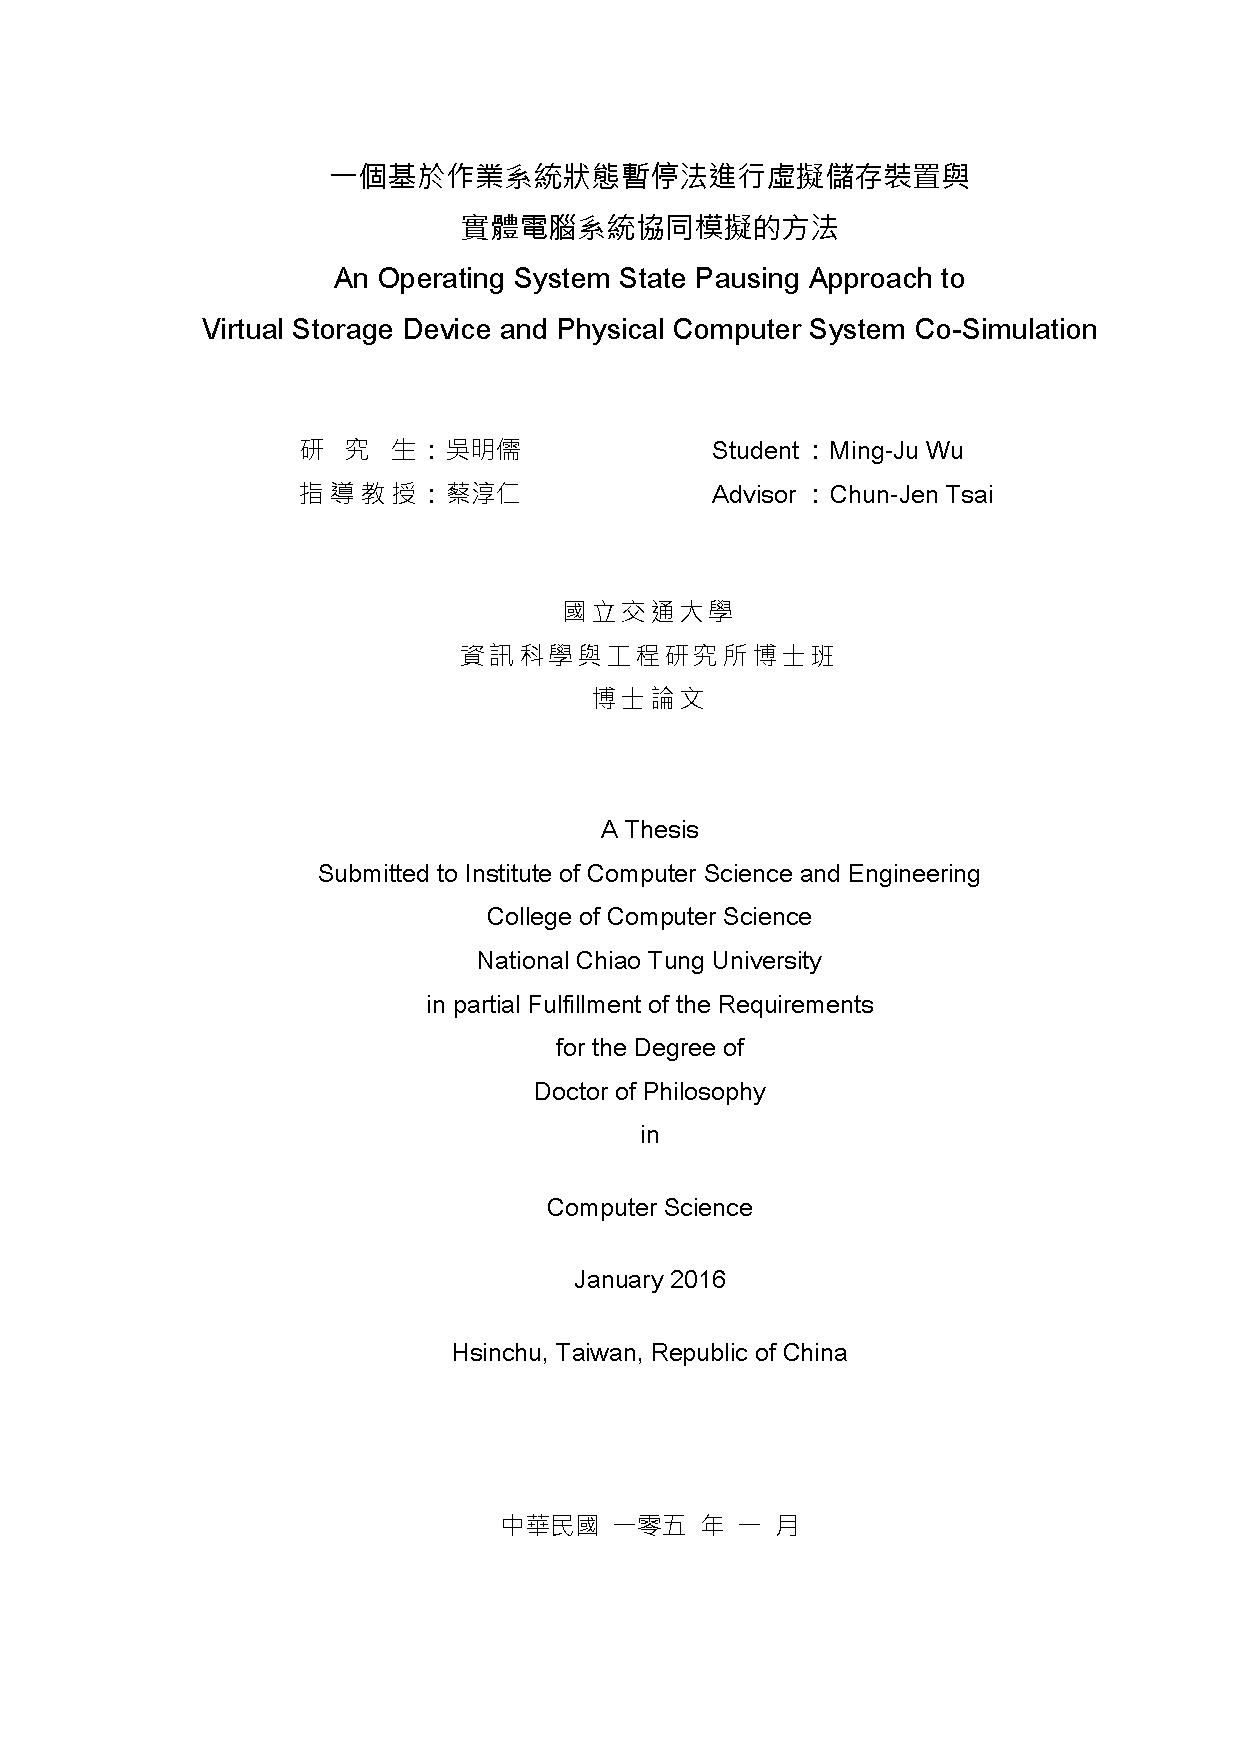
\includepdf[pages={1}]{書名頁-30mm-20mm.pdf}

\pagenumbering{roman}

\begin{abstractCH}

此篇論文提出了一個創新的作業系統狀態暫停方法,可以使得模擬出來的虛擬儲存裝置與實體電腦系統在離散時間上進行協同模擬。

儲存裝置仿真是對作業系統提供一個模擬出來的虛擬儲存裝置,並且使這個虛擬的儲存裝置可以像真實的裝置一樣的被作業系統使用。虛擬儲存裝置處理各I/O請求所需要的時間,是由一個描述儲存裝置特性以及效能的磁碟模型所定義。在傳統的儲存裝置仿真系統中,因為作業系統是在連續的時間軸上不間斷的在運行,且系統時間也是實時的在前進,因此儲存裝置仿真系統在模擬每一個I/O請求時,都必須要能夠在該I/O請求的回應時間內完成。如果儲存裝置仿真系統花費在模擬一個I/O請求的時間超過該I/O請求預定的回應時間,那麼作業系統所觀測到的儲存裝置的速度,就會慢於磁碟模型所定義目標。這樣的時間限制,對於傳統的儲存裝置仿真系統而言會造成模擬較高速的儲存裝置的困難。

利用這篇論文所提出的作業系統狀態暫停方法,進行虛擬處存裝置與實體電腦系統的協同模擬,可以解決傳統儲存裝置仿真系統必須在有限的時間內處理每個I/O請求的時間限制的問題。實際的做法為,每當儲存裝置仿真系統需要進行磁碟模型模擬以及建構I/O回應時,就透過論文中所提出的方法將作業系統的狀態進行暫停。如此一來,不論儲存裝置仿真系統花費了多少時間來處理每一個I/O請求,對於作業系統而言,都不會影響到其所觀測到的虛擬儲存裝置的速度以及特性。此外,因為在進行協同模擬時,作業系統以及軟體程式都是直接在真實的電腦硬體上執行,因此利用這樣的協同模擬環境進行實驗,能夠真實的保留目標硬體平台的效能與特性。

這篇論文利用所提出的協同模擬方法,建置了兩個全系統的協同模擬環境。(1) 第一個環境是一個全系統的協同模擬器,在這個協同模擬器中,虛擬儲存裝置的模擬器直接執行在目標作業系統上。這個協同模擬器的主要目的是讓開發者能夠以真實的測試資料以及量測值來對儲存系統進行評估。實驗數據顯示,所提出來的協同模擬器可以達到比實時速度快四十五倍的模擬速度。(2) 第二個協同模擬環境的主要目的是可以用來評估當一個電腦系統在配置了不同的儲存裝置時的整體效能。為了減少儲存裝置模擬器對於目標電腦系統的效能以及特性造成的影響,進而提高系統效能預估的準確度,儲存裝置模擬的主要工作交給了另外一台獨立的電腦來處理。實驗數據顯示,利用此協同模擬環境進行全系統效能評估的各項預測結果,與對照組環境所測得的結果之間的誤差皆小於百分之二。


\end{abstractCH}
\begin{abstractEN}

This dissertation proposes a novel operating system (OS) state pausing methodology that can be used to enable the co-simulation of virtually simulated storage device and physical computer system in the discrete-time domain. 

In storage device emulation, the emulated virtual storage device appears to the OS as a real storage device. The service timings of the emulated storage device are determined by a disk model which simulates the characteristics and performance of the target storage device. For the conventional storage device emulators, because the OS is running continuously in the real-time domain, the amount of time that the disk emulator can spend on processing each I/O request is limited by the servicing time of the corresponding I/O request. If the processing of an I/O request takes longer than the servicing time of the I/O request, then the OS would perceive a storage device that has a slower performance than the intended target. This real-time timing constraint can make emulating high-speed storage devices a challenge for conventional storage device emulators.

By utilizing the proposed OS state pausing co-simulation methodology for emulating storage devices, the timing constraints faced by the conventional storage device emulators can be avoided. By pausing the state of the OS whenever the storage device emulator is busy, the emulator can spend as much time as it needs for processing each I/O request without affecting the performance of the emulated storage device as perceived by the OS. In addition, because the OS and application programs are executing directly on the physical computer hardware, the performance characteristics of the real system can be taken into account during the co-simulation process.

In this dissertation, two co-simulation environments are constructed using the proposed OS state pausing methodology. (1) The first environment is a full-system co-simulator that runs the storage device emulator directly on the OS that the emulated storage device is plugged into. The main focus of this co-simulation environment is to allow realistic workloads and system-level metrics to be used for evaluating storage subsystem designs. With the experimental configuration, the proposed co-simulation environment has achieved simulation speed of up to 45 times faster than real-time. (2) The second co-simulation environment is focused on predicting the overall system performance of a particular computer system when different storage devices are available. To minimize the disturbances that the storage device emulator will have to the target system, and therefore improve the prediction accuracy, the work of storage device emulation is offloaded to an external computer. Experimental results show that the full-system performance benchmark results predicted using the proposed storage device emulator are within 2\% differences compared to the results from the reference system.

\end{abstractEN}

% For 列印
\newgeometry{twoside,top=2.5cm,left=3cm,bottom=2.5cm,right=2cm}

\onehalfspacing

\tableofcontents

\doublespacing

\listoffigures

\listoftables

%\listofalgorithms

\doublespacing

\mainmatter

\uchyph=0
% stop hyphenation of upper-case words.

\chapter{Introduction}

NAND flash storage devices are widely used in both embedded and server applications. The research results from the related fields, such as~\cite{Chang:2010}, \cite{Wu:2010}, and \cite{Chang:2012}, have helped to fuel the continuous improvements to the design and performance of NAND flash storage devices. Other types of non-volatile storage devices, such as PCM (Phase-Change Memory)~\cite{Zilberberg:2013}, MRAM (Magnetoresistive RAM), and FeRAM (Ferroelectric RAM)~\cite{Doh:2007}, are also being actively studied. Recently in 2015, Intel Corp. and Micron Technology Inc. have launched a new class of non-volatile memory called 3D Xpoint~\cite{wiki:3DXpoint}. 3D Xpoint has a stackable and transistor-less design, and it is claimed to have the potential of being up to 1,000 times faster than NAND flash and 8 to 10 times denser than DRAM. Therefore, it can be expected that there will be an ever increasing number of storage elements to choose from for building storage subsystems.

From a system-level perspective, a storage subsystem is consists of the physical storage device hardware and the software modules in the OS that control how the storage hardware is utilized. In particular, the software modules can include components such as the file-system layer, I/O scheduler, volume manager, block device driver, etc. The storage subsystem is driven by I/O workloads generated by application programs and activities internal to the OS, such as demand paging and memory swapping.

The design and characteristic of storage subsystems can have great influences in determine the overall system performance and end user experience in many scenarios~\cite{Kim:2012}. Benchmarking a storage component in isolation or with overly simplified system-level models can result in inaccurate performance evaluations. While theoretical analysis or simulation using abstract models can provide quick estimates on how different storage subsystems might affect the overall system performance, the accuracy of these approaches can be rough and can therefore lead to design conclusions that are contradictory to the real-world results~\cite{Thekkath:1994}. It has been shown that when simulating using abstract models, complex system-level interactions can hide or reduce the predicted effects of new storage subsystem designs~\cite{Ganger:1998}.

As illustrated in Figure~\ref{fig:full-system workload}, when designing storage subsystems, it is desirable that the engineers will be able to evaluate the design choices with the overall system-level behaviors in mind. For example, computer system architects might want to know how storage subsystem of different characteristics will affect the overall system performance. For storage device designers, it would be desirable that they can test simulated storage devices that are not yet available with realistic workloads so that early stage design trade-offs can be made with the overall performance in mind.

\begin{figure}[htpb]
	\centering
	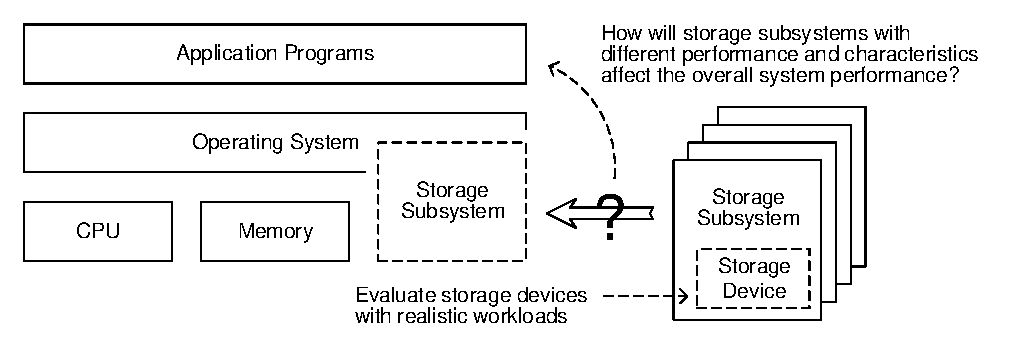
\includegraphics[width=\textwidth]{figures/Full-system.pdf}
	\caption[Evaluating storage subsystems in full-system context.]{\label{fig:full-system workload}The behaviors of the OS and application programs should be considered when trying to evaluate storage subsystems and storage devices.}
\end{figure}

When benchmarking storage subsystems, being able to use the real OS and application programs for generating the workloads can help in considering as much of the system-level behaviors as possible. Furthermore, since the instruction codes of the OS and application programs are run by the CPU, there are never truly pure I/O-bound workloads. For example, a workload that is perceived as I/O-bounded when executing on a faster computer can become CPU-bounded when being run on a computer with a slower CPU. That is, the speed of the hardware which the  OS and application programs run on can also affect the benchmarking results. Therefore, depending on the accuracy required for the performance predictions, the behaviors of the underlaying hardware, such as the CPU and memory subsystems, should also be considered in enough detail.

\section{The Problem and Motivation}

The problem that this dissertation sets to solve is to provide a full-system performance evaluation environment that can be used to experiment with prototype storage devices. while accurately taking into account the system-level behaviors of a computer system. Ideally, the full-system performance evaluation environment should consider as much of the system-level behaviors as possible, such as the behaviors of the OS, the benchmarking applications, and the performance of the underlying hardware that runs the software.

One of the conventional approaches that permits system-level evaluation of prototype storage device is storage device emulation. In this approach, a prototype storage device is constructed and made available to the OS of the target computer system. To the OS, the prototype storage device can be interactive with just like a real storage device. Because the OS and application programs are run on the real hardware, the detailed behaviors of the hardware of the target system are automatically considered. One limitation of the storage device emulation approach is that because the storage device emulator needs to reply the I/O requests back to the OS in real-time, there exists a hard time limit on the amount of time that is permitted for simulating the response for each I/O request. The time limit is equal to the intended response time of each I/O request. If the storage device emulator cannot complete the processing of an I/O request in this time limit, then the OS will perceive a storage device that is slower than intended. Therefore, it can sometimes be challenging or even impossible to emulate faster storage devices.

Complete machine simulation is another approach that allows the evaluation of prototype storage devices in full-system contexts. In complete machine simulation, a detailed simulation model of the target computer hardware, including the virtual storage device, is constructed and simulated in the discrete-time domain. The simulation model is detailed enough to run the real OS and application programs and should have execution timings close to the hardware of the target system. Since everything is simulated in the discrete-time domain, the speed of the storage device that can be modeled will not be constraint by the speed of the simulation host. That is, storage device of any speed can be studied with the complete machine simulation approach. However, one problem with this approach is that it can take great amount of effort for constructing and validating the detailed complete machine simulation model. Furthermore, depending on the complexity of the simulation model the simulation speed can be orders of magnitude slower than the real hardware. 

The observation and motivation of this dissertation is that the real hardware of the target computer system already encompasses the most truthful model of the desired complete machine behaviors, if the real hardware can be used as part of the complete machine simulation model for performing full-system performance evaluations, then the efforts needed for constructing and validating the simulation model of the target computer hardware can be avoided. In addition, executing the OS and application programs on the real hardware will be much faster than running them on virtually simulated hardware models.

\section{Thesis Statement}

This dissertation proposes a novel OS state pausing methodology for permitting the co-simulation of virtually simulated storage devices with the real OS and application programs running on real computer hardware. By utilizing the proposed methodology to perform full-system performance evaluations, the detailed simulation model of the target computer hardware does not need to be constructed. Furthermore, because the co-simulation is performed in the discrete-time domain, the speed of the virtual storage device that can be simulated will not be limited by the performance of the available hardware.

\section{Overview of the Dissertation}

When evaluating storage subsystems, the workloads and metrics used are important to the quality of the performance prediction results. Ideally, the storage subsystem should be evaluated in a full-system context which takes into account the detailed behaviors of the OS, the application programs, and the underlying hardware that runs the software.

Several approaches that are conventionally used by engineers and researchers for evaluating storage subsystems are discussed. The approaches that are discussed includes: (1) benchmarking with I/O traces, (2) complete machine simulation, and (3) storage device emulation. The shortcomings of these approaches are also discussed.

This dissertation proposes a novel way of pausing the state of the OS that is running on real hardware so that the OS and application programs can be co-simulated with virtually simulated storage devices in the discrete-time domain. The state of the OS can be considered to be the combined state of all the processes running in the OS and the timer and counter values observed by the OS. By freezing the execution of all the processes running in the OS and the advancement of the timer and counter hardware, the state of the OS can be paused. By carefully synchronize the state progression of the OS with the virtually simulated storage device, a full-system co-simulation environment can be constructed.

In this dissertation, the proposed OS state pausing methodology for co-simulating virtual storage device and real computer system is utilized in two usage scenarios:

\begin{enumerate}
	
	\item In the first usage scenario, a full-system co-simulation environment is built by using the proposed OS state pausing methodology to perform co-simulation of simulated virtual storage device with the OS and application programs running on real computer hardware. The full-system co-simulator allows the simulated storage device to be evaluated using realistic workloads generated by real OS and application programs. Higher level metrics such as elapsed user time and quality of service (QoS) at the application level can be used to benchmark the storage subsystem. By fast-forward the simulation time when the entire system is doing noting but waits in the CPU idle loop for the next event to arrive, the proposed full-system co-simulator can achieve faster than real-time simulations. The proposed full-system co-simulator has demonstrated up to 45$\times$ faster than real-time simulation speed in the experimental setup.
	
	\item In the second usage scenario, a storage device emulator based on the proposed OS state pausing approach is implemented for the Linux OS on the ZedBoard platform.
		
	In the proposed storage device emulator, a virtual storage device is emulated and made available to the OS at the block device driver level. The state of the OS is paused whenever the storage device emulator is busy processing I/O requests from the OS. Because of the pause made to the OS state, the storage device emulator can take as long as it needs for preparing each I/O response without affecting the perceived I/O response time by the OS. This allows prototype storage devices of any speed to be made available to the OS for full-system performance evaluation without being constraint by the speed of the hardware used for emulating the storage device.
	
	The proposed emulator allows the researchers to be able to predict the overall system performance of a particular embedded system, in the case of this dissertation, the ZedBoard platform, when different storage devices are used. The accuracy of the proposed storage device emulator is compared to a RAMDISK based reference system. The evaluation results from the proposed storage device emulator are shown to be within 2\% differences to the reference system.
	
	The storage device emulator takes a two part design. The work of simulation of the storage device model and persistence of the actual data is offloaded to another computer as to minimize the impact on the target system that the storage device is to be emulated. In particular, the size of the simulated storage device is not limited by the available storage space on the target system.

\end{enumerate}

\section {Contributions}

This dissertation makes three main contributions:

\begin{enumerate}
	\item An OS state pausing methodology is proposed that allows virtually simulated virtual storage devices to be co-simulated with real OS and application programs running on real computer hardware.
	
	\item A full-system co-simulator based on the proposed virtual storage device and real computer system co-simulation methodology is built and discussed in detail. The full-system co-simulator can be used for evaluating storage subsystem designs using realist workloads and system-level metrics.
	
	\item A storage device emulator is built using the proposed virtual storage device and real computer system co-simulation methodology~\cite{Wu:2015}. The target system is the ZedBoard platform running the Linux OS. The proposed storage device emulator allows the the prediction of the overall system performance of the target system when different storage devices are available. The full source code of the proposed storage device emulator is made available to the public domain\footnote{\url{http://www.cs.nctu.edu.tw/~cjtsai/research/nctusde}}.
	 
\end{enumerate}

\section {The Organization}

The remainder of the dissertation is organized as follows. Chapter~\ref{ch:2} discusses several approaches that are conventionally used for evaluating storage subsystems designs. Previous works related to storage subsystem performance evaluation are also discussed. Chapter~\ref{ch:3} introduces the concept of OS state pausing and how it is used in the co-simulation of virtually simulated storage device and real computer system. Chapter~\ref{ch:5} describes a full-system co-simulator based on the OS state pausing co-simulation approach. Chapter~\ref{ch:6} describes a storage device emulator based on the OS state pausing co-simulation approach. Chapter~\ref{ch:7} summarizes the contributions of this dissertation and suggests some directions for future research.


\chapter{Previous Work}
\label{ch:2}

Section~\ref{sec:ch2-convetional-approaches} discusses the approaches that are conventionally used for evaluating storage subsystem designs. Section~\ref{ch2:summary} gives a summary of the related works.

\section {Conventional Approaches to Storage Subsystem Evaluation}
\label{sec:ch2-convetional-approaches}
\subsection {Simulation with I/O Traces}
\label{sec:ch2-simulation-with-IO-traces}

I/O traces are often used by designers to evaluate the performance of storage subsystem designs due to its simplicity. In this method, I/O requests are recorded on a real system and are then played back in a simulation environment to drive a standalone model of the storage subsystem of interest. Ganer and Patt~\cite{Ganger:1998} have investigated on issues associated with using standalone models for evaluating storage subsystem designs. In general, doing performance predictions using standalone storage subsystems models in isolation without considering the system-level behaviors can have the following two problems:

\begin{itemize}
	\item The workloads used for benchmarking are often not representative of the reality~--- The conventional methodology of generating benchmark workloads using I/O traces often ignores feedback effects between the storage subsystem and the workload source since the workloads are generated offline. Due to lack of system-level models, the I/O traces are often played back using either open or closed subsystem models. In the open subsystem models, the I/O requests are assumed to have predetermined arrival times. That is, the changes to the completion times of I/O requests do not have effect on the arrival of subsequent requests. In the closed subsystem models, subsequent I/O requests are assumed to be generated as soon as the previous requests have been completed. In both the open and closed subsystem models, the arrival pattern of the I/O requests is always the same as when they are recorded on the real system. However, in real systems, the completion time of each individual I/O requests can affect the pattern or arrival times of subsequent requests.

	\item Metrics used for measuring standalone storage subsystem performance are not always good indicators of the overall system performance~--- When standalone storage subsystem model is used for performance predictions, the metrics that can be used for performance measurement is limited. For example, it is not possible to measure the overall system performance using the elapsed time or throughput of the user tasks. Improvement to the metrics that can be measured using standalone models, such as the response time and throughput of I/O requests, cannot always be used as the indicator to the improvement of the overall system performance.
\end{itemize}

\subsection{Simulation with Abstract System-Level Models}

The problems associated with using standalone storage subsystem models can be alleviated by incorporating system-level models in the simulation. In this approach, system-level trace, instead of I/O-level trace, of a real system is recorded and played back in a simulation environment which also models the system-level behaviors of the real system.

Some of the system-level behaviors that can affect the performance of a storage subsystem as perceived by the user are discussed as follows. When trying to predict the performance of a storage subsystem, depending on the accuracy required by the prediction results, some or all of these system-level behaviors should be considered.

\begin{description}
	\item[I/O scheduling] In modern operating systems, I/O requests can be reordered or merged before actually being submitted to the underlying storage devices. This behavior is called I/O scheduling and is usually done for optimizing and balancing I/O request service times. The operation of the I/O scheduling algorithm is a dynamic behavior that depends on the state of the request queue and the arrival time and the order of the I/O requests. Benchmarking using pre-recorded I/O traces can overlook the impact of the I/O scheduling process on the storage subsystems.
	
	\item[File system mapping layer] Most real world applications are designed around file systems and do not access the underlying raw storage devices directly. Depending on the characteristics of the workload, using different file system mapping layers can have dramatic effects on the performance of the storage subsystems. Without modeling the behaviors of the file system mapping layer, it is sometimes not possible to accurately predict the performance of a storage subsystem design.
	
	\item[Dynamic data partitioning] A tiered storage subsystem have storage devices of different sizes and speeds; it will decide at run-time where to store the incoming I/O requests and will also move data among different tiers of storage devices. Benchmarking with prerecorded I/O traces cannot reproduce this kind of dynamic data partitioning behavior.
	
	\item[Caching] Caches are used at various layers in a system to improve performance; it can affect the actual workloads hitting the lower-level layers. For example, the I/O requests that actually hit the underlying storage devices are the ones that missed the upper layer caches. Depending on the target system’s cache configurations, I/O traces prerecorded with different system configurations might not be representative enough for testing the target system.
	
	\item[Virtual memory swapping] On operating systems that implement virtual memory, additional workloads could be imposed on the storage subsystem when memory swapping occurs. The overall performance of the storage subsystem can be affected by such additional workload.
	
	\item[Multi-tasking] In a multi-tasking system, the aggregated I/O workload submitted to the storage subsystem can be generated by concurrently running applications. Depending on the characteristics of the applications, for example, I/O-bound or CPU-bound, and the task scheduling algorithm, the aggregated I/O workload that will be generated cannot easily be simulated by I/O tracing techniques. 
\end{description}

It can be expected that modeling all of the aforementioned behaviors for simulation can take a great deal of work. Furthermore, even if one takes the effort to build and validate the abstract models for all of the essential system-level behaviors in a simulator, the chosen runtime parameters for each abstract model may not precisely simulate the real system. Depending on how subtle the design choices are, the differences can lead to inaccurate performance predictions and therefore wrong conclusions.

\subsection{Complete Machine Simulation}

\begin{figure}[htpb!]
	\centering
	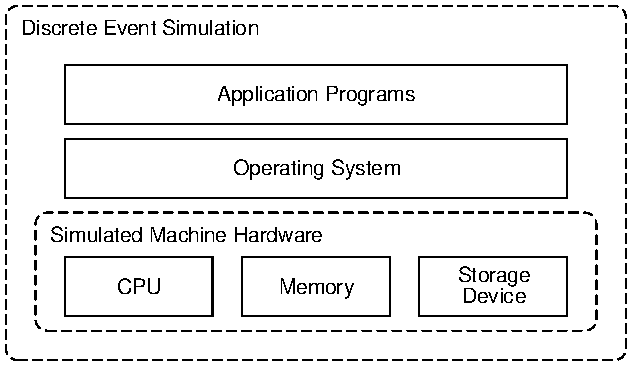
\includegraphics[width=0.65\textwidth]{figures/complete-machine-simulation.pdf}
	\caption{\label{fig:complete-machine-simulation}Complete machine simulation.}
\end{figure}

Complete machine simulation is one of the approaches which can allow the overall system performance to be evaluated with simulated storage devices that are not yet available. The concept of the complete machine simulation approach is illustrated in Figure~\ref{fig:complete-machine-simulation}. With complete machine simulation, a simulation model of the target machine hardware, including the storage device of interest, is first constructed.  The OS and application programs are then executed on the simulated machine hardware to study the overall system performance. An attractive attribute of the complete machine simulation approach is that it can be used for studying a wide range of system configurations – anything that can be modeled and simulated can be studied. Because the entire virtual machine model is simulated in the discrete-time domain, the performances and characteristics of the storage devices that can be simulated will not be limited by the performance of the simulation host. For example, it is possible to use a slower conventional hard disk drive for simulating large and faster solid-state drive (SSD) storage devices.

Unfortunately, one problem with the complete machine simulation approach is that the simulation speed of the complete machine model can be much slower than the speed of the native machine hardware. For example, in the SimOS environment~\cite{Rosenblum:1995}, simulation using the detailed CPU model can be 3 to 4 orders of magnitude slower than running the same workload on the native host.

Another problem with the complete machine simulation approach is the difficulties and efforts that are involved in constructing accurate complete machine models~\cite{Gibson:2000}, \cite{Gutierrez:2014}. Although there are simulators that are capable of running a sophisticated operating system, there are reports that show that their accuracy may differ from the real system when simulating memory-intensive tasks due to lack of exact memory subsystem models. Moreover, the internal design details of commercial SoCs might not be made publicly available by its manufactures~\cite{Eklov:2011}. In particular, accurate memory subsystem models (including the cache controller, the memory controller, and the DRAM models, etc.) are often not available for commercial embedded SoCs. For example, in~\cite{Butko:2012}, the differences in the real performance and simulated performance with the default models of the popular GEM5 simulator can be as large as 17.94\%.

%TODO: 
%---> Please note that ... Complete machine simulators that do not model accurate timings of the target hardware cannot be used for performance evaluations. For example, QEMU... copy some text from author's response here...

\subsection{Timing-Accurate Storage Device Emulation}
\label{sec:ch2-timing-accurate}

Timing-accurate storage device emulation is another approach that can be used for evaluating the overall system performance with simulated storage devices that are not yet available~\cite{Griffin:2002}. In timing-accurate storage device emulation, an emulated storage device is made available to the OS which is executing on the real machine hardware. The OS can interact with the emulated storage device similar to with a real storage device. The service timings of the emulated storage device are determined by a disk model which models the behavior of the target storage device. When an I/O request is submitted to the emulated storage device, the storage device emulator will need to carry out the following tasks:

\begin{enumerate}
\item Compute the response time of the I/O request by simulating the disk model.
\item Handle the actual data of the I/O request. If the I/O request is a write request, then the actual data is stored to the backing storage. Otherwise, the actual data is retrieved from the backing storage.
\item	Reply the I/O response to the OS at the corresponding service time as determined by the disk model.
\end{enumerate}

The conventional storage device emulators can conceptually be classified into two types of designs:
\begin{enumerate*}[label=(\roman*)]
	\item local virtual storage device emulation, and
	\item remote actual storage device emulation.
\end{enumerate*}
These two types of designs will be discussed in the follow subsections.

\subsubsection{Local Virtual Storage Device Emulation}

\begin{figure}[htpb!]
	\centering
	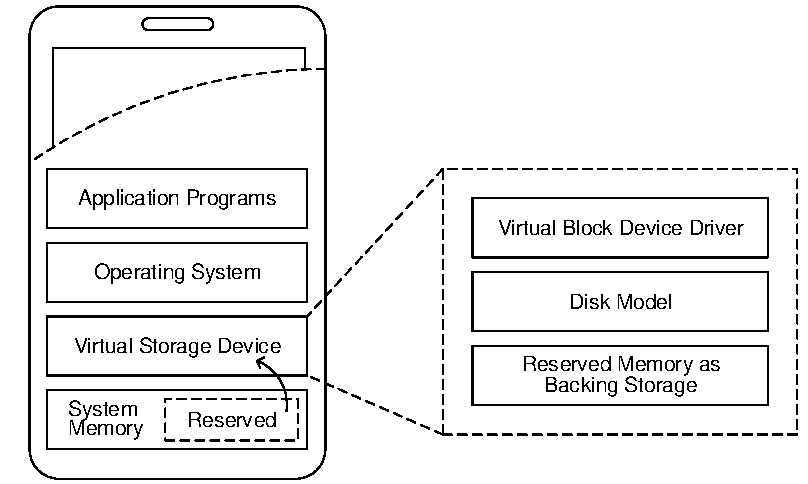
\includegraphics[width=0.8\textwidth]{figures/local-virtual-emulation.pdf}
	\caption{\label{fig:local-virtual-emulation}Local virtual storage device emulation.}
\end{figure}

An overview of the local virtual storage device emulation design (which will be referred to as the local emulation design for short for the rest of this dissertation) is illustrated in Figure~\ref{fig:local-virtual-emulation}. In the local emulation design, a virtual storage device is presented to the OS at the device driver level. The service timings of the emulated storage device are determined by a disk model which is simulated using the target system's CPU. A portion of the system memory is reserved and used as the backing storage for persisting the actual data of the emulated storage device.

While the local emulation design is convenient to implement, it has two notable limitations:

\begin{itemize}
	\item The size of the emulated storage device will be limited by the amount of the system memory that can be reserved for the backing storage. Embedded systems are usually configured with no more than a few gigabytes of memory, and therefore can greatly limit the size of the benchmark workload that can be used for evaluation. Furthermore, reducing the amount of the system memory that can be used by the OS will affect the original behavior of the system. If the remaining system memory is under a certain threshold, it can also prevent the proper execution of the desired benchmark workloads.
	
	\item Because the disk model is simulated using the target system's CPU, the emulator will consume CPU cycles of the target system and therefore will affect the original system behavior. More importantly, if the time that it takes to simulate the disk model exceeds the targeted service time of the corresponding I/O request, then the emulator will fail to emulate the intended behavior of the target storage device.
\end{itemize}

\subsubsection{Remote Actual Storage Device Emulation}

\begin{figure}[htpb!]
	\centering
	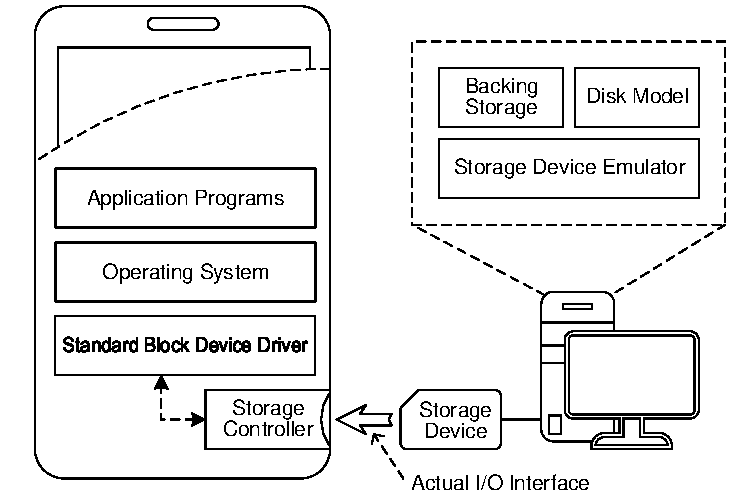
\includegraphics[width=0.75\textwidth]{figures/remote-actual-emulation.pdf}
	\caption{\label{fig:remote-actual-emulation}Remote actual storage device emulation.}
\end{figure}

An overview of the remote actual storage device emulation design (which will be referred to as the remote emulation design for short for the rest of this dissertation) is illustrated in Figure~\ref{fig:remote-actual-emulation}. In the remote emulation design, an actual storage device is emulated by the emulator software running on a separate computer and is presented to the OS at the actual I/O interface level. For example, if the target system has a Secure Digital (SD) card reader, then a storage device which is compatible to the SD standard can be emulated by the storage device emulator and inserted into the SD card reader of the target system.

Because the emulator software runs on a separate computer, the remote emulation design can overcome some of the problems faced by the local emulation design: Firstly, the size of the emulated storage device will not be limited by the size of the system memory available on the target system. It can be as large as the system memory or the backing storage available on the separate computer. Secondly, the CPU usage of the target system will not be affected by the emulator.

However, there are some limitations with the remote emulation design:

\begin{itemize}
	\item In both the local and remote emulation designs, the OS is running continuously in the real-time domain and the system time that the OS observes is progressing at the real-time speed. Therefore, in order to properly emulate the intended behavior of the target storage device, the conventional storage device emulators must be able to complete the processing of each I/O request in a timely fashion. The amount of time that is allowed for processing each I/O request is bounded by the service time of the particular I/O request. For example, if the computed service time of an I/O request is 1ms, then the total amount of time that can be used by the storage device emulator for simulating the disk model and accessing the backing storage cannot exceed 1ms. Otherwise, the performance of the emulated storage device will be slower than the intended target, which will lead to performance evaluation errors.
	
	\item The latency and bandwidth of the emulated storage device will be limited by the latency and bandwidth of the actual I/O interface. For example, the UHS-I bus interface defined by the SD standard has a maximum bus speed of 104MB/s, and therefore storage devices which are faster than 104MB/s cannot be emulated over the UHS-I interface. This kind of limitation can prevent the emulation of faster storage devices over existing I/O interfaces.
	
	\item The features that can be supported by the emulated storage device will be limited by the characteristics of the actual I/O interface. For example, because the SD interface protocol does not support more than one outstanding I/O requests concurrently, storage devices which have features such as Native Command Queuing (NCQ) cannot be emulated over the SD interface.
\end{itemize}

\section {Related Work}
\label{ch2:summary}

Proper evaluation of storage subsystems is not an easy task. Traeger et al.~\cite{Traeger:2008} have proposed a set of guidelines for proper storage subsystem performance evaluations.
% TODO: Summarize the guide lines here.
Using the guidelines as the evaluation criteria, they have surveyed 415 file system and storage benchmarks from a selection of conference papers between the year 1999 and 2007. The selected benchmarks are all conducted on real machine environments. They have found that most benchmarks are flawed and could give the readers wrong impressions on the real performance of the storage subsystems under test and even lead to incorrect design conclusions. From the guidelines, it can be clearly seen that it is important that the system-level behaviors are taken into account when performing storage subsystem evaluation.

In the work of Ganger and Patt~\cite{Ganger:1998}, they have constructed abstract system-level model that contains necessary host system component modules with appropriate details for generating workloads for benchmarking storage subsystems. System-level traces, instead of I/O traces, are recorded on real system and played back using the abstract system-level model for generating workloads to drive the storage subsystem module.

Instead of using purely abstract models for system-level simulation, Thekkath~\cite{Thekkath:1994} incorporated real file system code into the simulation system. In his approach, I/O traces are gathered on real systems and are used to drive the real file system code in the simulation process for generating I/O requests.

An alternative to using abstract system-level models for performing storage subsystem evaluations is to use complete machine simulation. The SimOS environment~\cite{Rosenblum:1995}, \cite{Witchel:1996}, \cite{Rosenblum:1997} is a complete machine simulator which can simulate the hardware of an SGI machine in enough detail to run the Irix OS. SimOS supports switching among a number of hardware component models which are different in terms of modeling detail and accuracy. The less detailed models can run faster and can be used to boot and position the system into a state at which interesting workloads will begin. The simulation can then switch to use a more accurate model for detailed profiling. Griffin et al.~\cite{Griffin:2000} has integrated a MEMS-based storage device simulator into the SimOS environment for studying the performance and characteristics of MEMS-based storage devices. Although complete machine simulation does allow the actual OS and real applications to be run on the simulated machine hardware, it can run much slower than the real system. Furthermore, building and maintaining accurate complete machine simulation models could take substantial amount effort.

Timing-accurate storage emulation has been explored in detail by Griffin et al. \cite{Griffin:2002}. Memulator allows researchers to explore with nonexistent storage devices and take end-to-end measurements in full-system contexts. Memulator can use either the memory of the local machine or a networked machine as the backing storage for the emulated disk. Their work gives support that storage device emulation is an effective method for studying the overall system performance with simulated virtual storage devices. In their remote emulation setup, the emulator is executed on a standalone computer and connected to the target system over the SCSI interface. The DiskSim simulator~\cite{Bucy:2008} is used for simulating the service times of the Seagate Cheetah X15 hard disk drive. Experimental results show that the benchmark results measured with the emulated storage device are close to the results measured with the real storage device.

In the work of Maghraoui et al.~\cite{ElMaghraoui:2010}, a local emulation type storage device emulator is developed to emulate flash based SSD for the AIX OS. The emulator is implemented as a dynamic loadable kernel module and appears to the OS as a disk device. A chunk of system memory is pined for use as the backing storage, and high resolution nanosecond granularity timers are used for simulating the delays of the I/O operations. Lee et al.~\cite{Lee:2012} have proposed another local emulation type SSD emulator. The target platform is the Linux OS and it uses a user mode SSD simulation engine for calculating the latencies for the I/O requests. The backing storage used can be either the system memory or some other external DRAM-based storage devices.

David~\cite{Agrawal:2012} is another local emulation type storage device emulator which is mostly concerned about the required backing storage size for emulating large storage devices. The main idea of David is to reduce the data that needs to be saved to the backing storage so that larger storage devices can be emulated using less storage space. The key idea is that for certain types of benchmark workloads, the actual content in the file system files can be omitted and only file system metadata needs to be persisted onto the backing storage. By not persisting the actual content in the files, David is able to reduce the storage size requirements by orders of magnitude. David has been demonstrated to work with the ext3 and the btrfs~\cite{wiki:btrfs} file systems, and in theory, it can be extended to work with other types of file systems.

VSSIM~\cite{Yoo:2013} is a virtual machine (VM) based SSD simulator which makes emulated SSD devices available to the VM. The emulated SSD device appears to the VM as a storage device connected to the IDE interface. VSSIM runs in real-time and allows the user to measure both the host performance and the SSD behavior under various design choices. The design of VSSIM can conceptually be classified as similar to the remote emulation design. The difference is that the target machine that the emulated storage device is ``connected'' to is a VM, and therefore VSSIM does not need to emulate the actual electrical signals of the IDE interface.

Finally, Canon et al.~\cite{Canon:1980} extended the standard virtual machine (VM) environment to include virtual time emulation. In contrast to the conventional VM environment, in which the real time of day (RTOD) clock is observed by the VM, the modified VM environment makes the VM to observe a virtual time of day (VTOD) clock. The VTOD clock progresses as program instructions are executed on the virtual CPU of the VM. In the modified VM environment, the system performance is evaluated against the VTOD clock. The VM environment proposed by Canon et al. can be viewed as analogous to the SimOS environment configured with the direct execution model, in which the machine instructions are executed on the native CPU whenever possible and that the internal architecture of the CPU is not modeled.


\chapter[Operating System State Pausing and Virtual Storage Device \\ Co-Simulation]{Operating System State Pausing and Virtual Storage Device Co-Simulation}
\label{ch:3}

This dissertation proposes a novel OS state pausing approach to storage device emulation that allows simulated virtual storage device to be co-simulated with OS and application programs running on real computer hardware. The key idea of the proposed approach is to modify the OS in a way that its execution state can be paused and resumed, even while the OS is being run on unmodified real computer hardware. This means that the flow of time that is observed by the OS and application programs can be controlled discretely and is no longer hardwired to the real-world time. By properly controlling the execution state of the OS and synchronizes it with the simulation progression of the virtual storage device, the simulated virtual storage device can be made to co-simulate with the real computer system that runs the modified OS in the discrete-time domain. The resulting co-simulation environment can be used for conducting studies on the simulated virtual storage device and the corresponding storage subsystem in realistic full-system contexts.

One way to understand the proposed co-simulation approach is that the real physical hardware is used as part of the full-system simulation model. In the complete machine simulation approach, a detailed model of the target system's hardware needs to be constructed and used for running the software programs. The hardware model needs to be detailed enough so that it can execute the real OS and application programs. It's performance characteristics also needs to be precise enough so that the performance evaluation results predicted using the complete machine model will be representative of the real world results. In other words, only achieving behavioral correctness with the simulated hardware model is not enough for conducting full-system performance evaluations.

With the proposed co-simulation approach, the OS is running on the real computer hardware. This means that the detailed characteristics of the CPU and memory subsystems will be taken into account when the co-simulation model is used for generating workloads towards the virtual storage device or for conducting full-system performance evaluations. Furthermore, utilizing the real hardware to run the software programs will be faster then running them on virtually simulated hardware models.

The key concept of the proposed co-simulation methodology is to control the execution state of the OS and make the OS to observe a virtual system time that is not hardwired to the real world clock. In the work of Gupta~\cite{Gupta:2006}, they proposed a technique called \textit{time dilation} to make the OS to observe a passage of time that is a constant time slower than the real-time clock. From the OS’s perspective, the physical resources in the external world will appear to be faster than their original speeds. For example, if the passage of time observed by the OS is slowed down by 10 times, then data arriving from a network interface at a physical rate of 1Gbps would appear to the OS as arriving at 10Gbps. They have demonstrated that \textit{time dilation} is an effective method for emulating network interfaces of different speeds to the OS for end-to-end system behavior experimentations. 

Although the proposed storage device emulator also makes the OS to observe a passage of system time that is different than the real-time clock, the goal and mechanisms are different from those of \textit{time dilation}:

\begin{itemize}
	\item  In \textit{time dilation}, the passage of system time is only slowed down by a constant factor but will never be stopped. In other words, the OS is always executing continuously. In contrast, in our proposed OS state pausing approach, the execution of the OS will be paused as necessary whenever the storage device emulator is busy processing the I/O requests. The goal of \textit{time dilation} is to trick the OS into believing that the external resources are faster than what they actually are. On the other hand, the goal of OS state pausing is to temporarily freeze the execution of the OS so that the storage device emulator can spend unlimited amount of time on processing the I/O requests.
	
	\item The slowing down of the passage of time in \textit{time dilation} is achieved by reducing the frequency that the timer interrupts are delivered to the OS and also by appropriately scaling down the hardware time counter that is used by the OS. For example, to slow down the passage of time observed by the OS by 10 times, the timer interrupt frequency is reduced by 10 times and the hardware time counter is also scaled down by 10 times. In comparison, pausing the state of the OS requires stopping the hardware time counter and preventing the CPU from doing any work for the OS.
	
	\item The design of the proposed storage device emulator can be extended with \textit{time dilation}. In the proposed emulator design, the OS can either be in the paused state or in the running state. When in the running state, it is possible to apply \textit{time dilation} so that the OS will observe that it is running on a CPU which is faster than the CPU of the target system. However, in order to keep our focus, we do not apply \textit{time dilation} to the proposed storage device emulator in this article.
\end{itemize}

The concept of OS state pausing is discussed in section~\ref{sec:controlling-OS-state}. Section~\ref{sec:OS-state-pausing-and-storage-device-emulation} gives an overview of how OS state pausing is used to allow virtual storage device to be co-simulated with real computer system running real OS and application programs. Section~\ref{sec:synchronization-granularity} discusses the synchronization considerations between the state of the simulated virtual storage device and the state of the OS. The idea of time-skipping the CPU idle loop, which can be used to accelerate the co-simulation process, is discussed in section~\ref{sec:time-skipping}.

\section{Controlling the Operating System State}
\label{sec:controlling-OS-state}

The key of being able to co-simulate the OS running on unmodified real computer hardware with simulated virtual storage device in the discrete-time domain is the ability to control the state progression of the OS. That is, we need to be able to pause and resume the running state of the OS on unmodified computer hardware.

\begin{figure}[htpb]
	\centering
	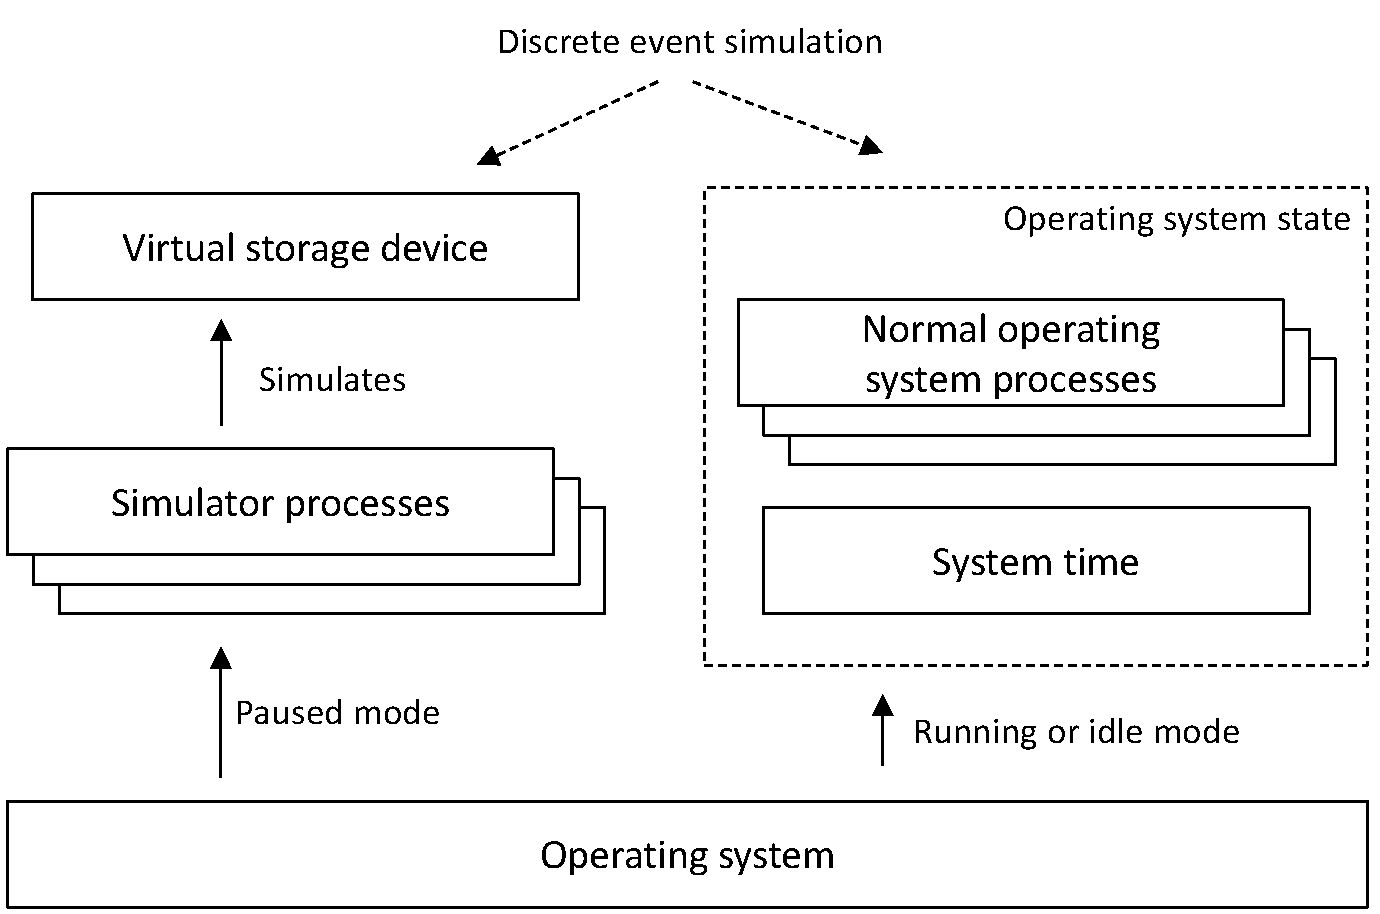
\includegraphics[width=0.8\textwidth]{figures/ch3-OS-state.pdf}
	\caption{\label{fig:ch3-OS-state}OS state pausing and discrete event simulation.}
\end{figure}

As illustrated in Figure~\ref{fig:ch3-OS-state}, the state of an OS can be viewed as composed of the combined state of all the normal processes running in the OS and the values in the clock counter and the hardware timers referenced by the OS. By freezing the execution of all the normal processes in the OS and stopping the clock counter and the hardware timers, the state of the OS is paused. The ``normal'' operating system processes are referring to the processes that are part of the original unmodified OS. On the other hand, the ``simulator'' processes are processes that do not exist in the original OS and are responsible for performing tasks such as storage device simulation while the OS is in the paused state.

By properly control the state progression of the OS, the OS can be co-simulated with the virtual storage device to form a full-system simulation environment. The OS can be put into one of the three following modes during the co-simulation process:

\begin{itemize}
	\item \textbf{Pause mode} --- In this mode, the progression of the OS state is frozen. All of the normal processes are prevented from being run on the CPU and the clock counter and hardware timers are paused. When in the paused mode, the system time that is perceived by the OS is no longer advancing and the CPUs are not performing any useful work for the OS. The simulator processes are executed only when the OS is in the paused mode, and therefore the execution of the simulator processes will not affect the original behavior of the OS.
	
	\item \textbf{Running mode} --- In the running mode, the OS state is advancing continuously with regarding to the real-world clock. That is, for every second that the OS is put into the running mode, the OS state is advanced one second into the future. In the running mode, the normal processes are selected to run on the CPU according to the task scheduling policy of the OS. All of the clock counter and hardware timers that the OS reference are operating normally.

	\item \textbf{Idle mode} --- The idle mode is a special case of the running mode. The OS is said to be in the idle mode when the OS is in the running mode but that the CPU is executing the CPU idle process. In this mode, all the normal processes excluding the CPU idle process will remain in the same states. Observe that while the OS is in the idle mode, the only OS state that is changing is the system time. Therefore, it is possible to fast-forward the system time to a future time point so that the simulation process does not spend unnecessary time waiting in the idle mode. The ``time-skipping'' feature what will be further discussed in section~\ref{sec:time-skipping}.
\end{itemize}

\section{Storage Device Emulation and Discrete Event Simulation}
\label{sec:OS-state-pausing-and-storage-device-emulation}

The proposed co-simulation methodology is based on the concept of storage device emulation and discrete event simulation. In the timing-accurate storage device emulation methodology of Griffin et al.~\cite{Griffin:2002}, a virtual storage device with timing behaviors matching the target device is plugged into the OS. The virtual storage device along with other modules in the OS forms the storage subsystem. The entire system operates in the real-time domain. Real applications running on the OS can be used for generating benchmark workloads towards the simulated storage device.

In the proposed methodology, a virtual storage device is emulated to the OS at the block device driver level and its simulation state is synchronized with the state of the OS. Whenever there is an I/O request received by the emulated storage device, the OS is put into the paused mode while the storage device emulator is busy preparing the I/O response. The OS is put back to the running mode when the timing for the I/O response is determined. A timer event that references the virtual system time is used to submit the I/O response to the OS when the corresponding response time has arrived. Because of the pausing made to the OS state, the OS and the virtual storage device can be viewed as being co-simulated together in the discrete-time domain.

In summary, the key difference between timing-accurate storage device emulation and the proposed co-simulation methodology is the time domain that the whole system operates in. In timing-accurate storage device emulation, the simulation time of the virtual storage device emulator is synchronized with the real-word clock. Both the OS and the virtual storage device are operating in the real-time domain. That is, the state of the entire system progresses according to the real-world clock. In contrast, in the proposed co-simulation approach, the OS and the virtual storage device are simulated together in the discrete-time domain.

The key advantages of the proposed OS state pausing full-system co-simulation approach compared to the timing-accurate storage device emulation approach are summarized as follows.

\begin{itemize}
	\item The OS state can be paused. This means that the storage device simulation module can take as long as it needs for preparing the I/O responses without affecting the performance of the storage device as perceived by the OS. In comparison, in the timing-accurate storage device emulation approach, each individual I/O request must be responded back to the OS at exactly the desired service time of the disk model. Otherwise, the emulated storage device will have a performance characteristic that is different from the intended target. In other words, the storage device simulation module must be able to prepare the I/O responses in real-time.

	\item It is possible for the proposed full-system co-simulation environment to be simulated at a speed that is faster than real-time. In the timing-accurate storage device emulation approach, the OS is operating in the real-time domain using the real-world clock as its system time. This means that the entire evaluation process is constrained to proceed at the real-time speed. On the other hand, with the proposed co-simulation approach, the OS state can be fast-forwarded to speedup the simulation process whenever the CPU is in the idle loop due to waiting for the I/O response from the emulated storage device.
\end{itemize}

\section{Synchronization Granularity}
\label{sec:synchronization-granularity}

In discrete event simulation, a simulation model of the target system is constructed and its state is changed by a chronological sequence of discrete events. The simulation model of the proposed full-system co-simulation environment contains two parts:
\begin{enumerate*}[label=(\roman*)]
	\item the OS running on the real machine hardware, and
	\item the storage device simulator.
\end{enumerate*}
During simulation, the two parts of the simulation model need be advanced in a synchronized fashion so the overall system behavior is correct. That is, the state progression of the OS needs to match with the state progression of the simulated storage device. For example, if the OS submits an I/O request to the simulated storage device at time $t$ and it takes the
device $\Delta t$ amount of time to complete the I/O request, then it is important that when the I/O response is replied back to the OS, the system time of the OS is at $t + \Delta t$.


In the conventional full machine simulation approach, the synchronization between the OS and the storage device is achieved automatically by running the OS on the simulated machine hardware model. Due to the storage device is part of the machine hardware model, the OS state will automatically be synchronized with the state of the storage device. Depending on the design, the state advancement of the entire simulation model can be progressing at different granularities. For example, it could be at the per clock cycle or the per CPU instruction levels. Although extremely accurate, this kind of fine-grained synchronization between the OS and the simulated device is not necessary for evaluating storage subsystem designs.

\begin{figure}[htpb]
	\centering
	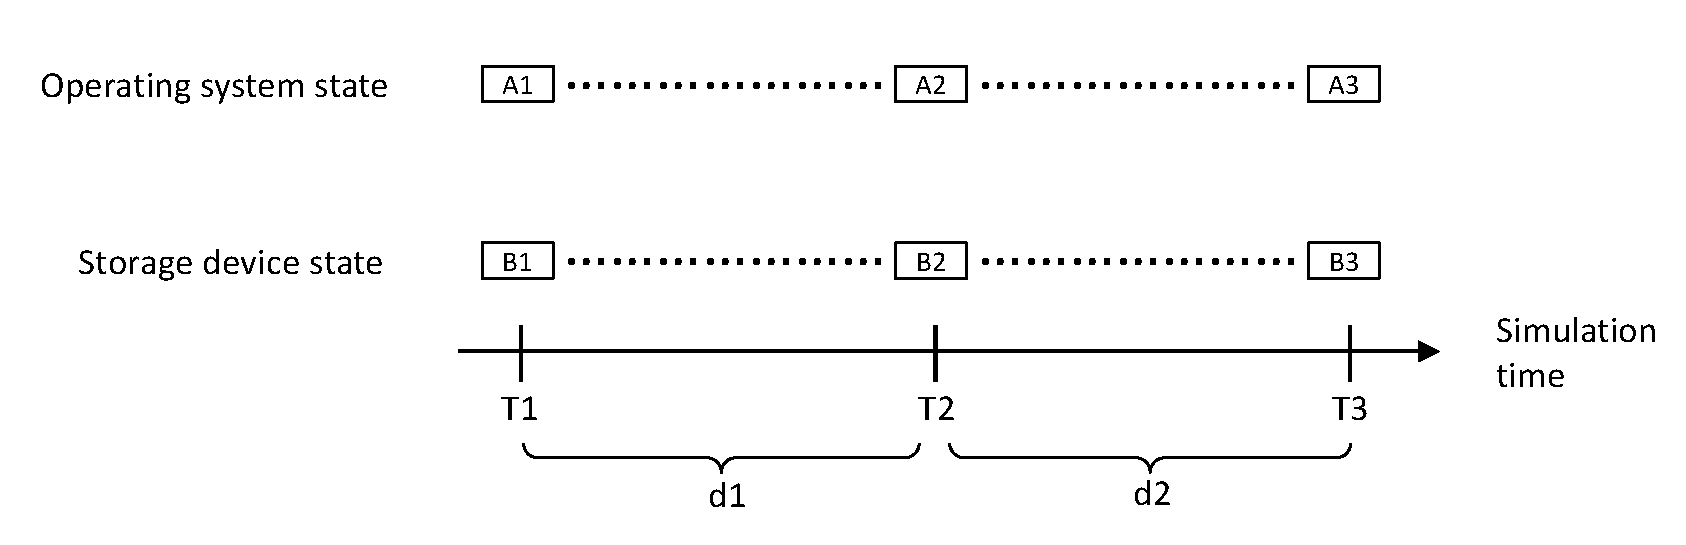
\includegraphics[width=0.95\textwidth]{figures/ch3-sychronization-granularity.pdf}
	\caption[Synchronization between the OS and the simulated storage device.]{\label{fig:ch3-sychronization-granularity}For evaluating storage subsystem designs, the states of the OS and the simulated storage device only need to be synchronized at the I/O event level.}
\end{figure}

The observation is that for evaluating storage subsystem designs, synchronizing the state of the OS and the state of the simulated storage device at the I/O event level is sufficient for capturing the overall system behavior. Figure~\ref{fig:ch3-sychronization-granularity} is used to explain this concept. Assuming that a simulation model that contains an OS and a storage device is being simulated, when the simulation begins at time point T1, both the OS and the storage device are in their initial states A1 and B1, respectively. After d1 amount of time, at simulation time point T2, the OS submits an I/O request to the storage device, and the storage device simulator determines that it requires d2 amount of time to process the I/O request. After d2 amount of time, the I/O response is replied back to the OS at simulation time point T3. Observe that for the purpose of evaluating storage subsystem designs, synchronizing the simulation states of the OS and the storage device at time point T1, T2, and T3 is sufficient for capturing the overall system behavior. That is, the co-simulation environment only needs to make sure that when the OS is at state A2, the storage device is at state B2; similarly, when the OS is at state A3, the storage device is at state B3. The intermediate states between A1 and A2, or A2 and A3, do not need to be explicitly synchronized with the intermediate states between B1 and B2, or B2 and B3. In other words, the co-simulation environment only needs to make sure that the entire simulation model is in a synchronized state when the OS is interacting with the simulated storage device. The intermediate states that the OS goes through internally do not need to be synchronized explicitly with the internal intermediate states of the simulated storage device.

\section{Time-Skipping --- Fast Forwarding the CPU Idle Loop}
\label{sec:time-skipping}

When the OS is in the idle mode, the CPU is simply waiting in an indefinite idle loop and not doing any useful work. That is, the OS is simply waiting for the system time to pass by so that some process will become runnable again. To speedup the simulation process, it is possible to time-skip the CPU idle loop by fast-forwarding the system time to a future time point. As soon as the OS enters the idle mode, the simulation kernel determines the future system time point at which there will be a process to become runnable again. The system time is then fast-forwarded to that future time point and the OS can get out of the idle mode immediately. This operation is called ``time-skipping'' the CPU idle loop.

Notice that the OS state will be the same when it finally leaves the idle mode either with or without applying the time-skipping feature to skip the CPU idle loop. This is because the only OS state parameter that will be changed while the OS is in the idle mode is the system time. The states of all the other processes in the OS will remain unchanged. Therefore, to the OS state, fast-forwarding the system time to a future time point at which some process will become runnable again is equivalent for the CPU to actually wait in the CPU idle loop and waits for the corresponding amount of time to pass by.

When the storage subsystem is being benchmarked, there will always be at least one process in the OS waiting in the sleep state. In general, the benchmark application could go into the sleep state because it is waiting for an I/O response from the storage device or it has voluntarily relinquished CPU for certain amount of time. In the first case, it means that the storage device simulation module will have registered a timer callback and is waiting for the corresponding time to arrive so that it can reply the I/O response to the OS. The storage device simulation module will be in the sleep state while waiting for the timer event to happen. In the second case, if the benchmark application has voluntarily relinquished the CPU, it will be woken up again when the corresponding amount of time has passed. In both cases, it will be possible to find the system time point to fast-forward to so that there will be a process to become runnable again. The co-simulation process can be determined to be ended when the benchmark application is finished and that there is no future time point to skip to when the CPU enters the idle loop.

\begin{figure}[htpb]
	\centering
	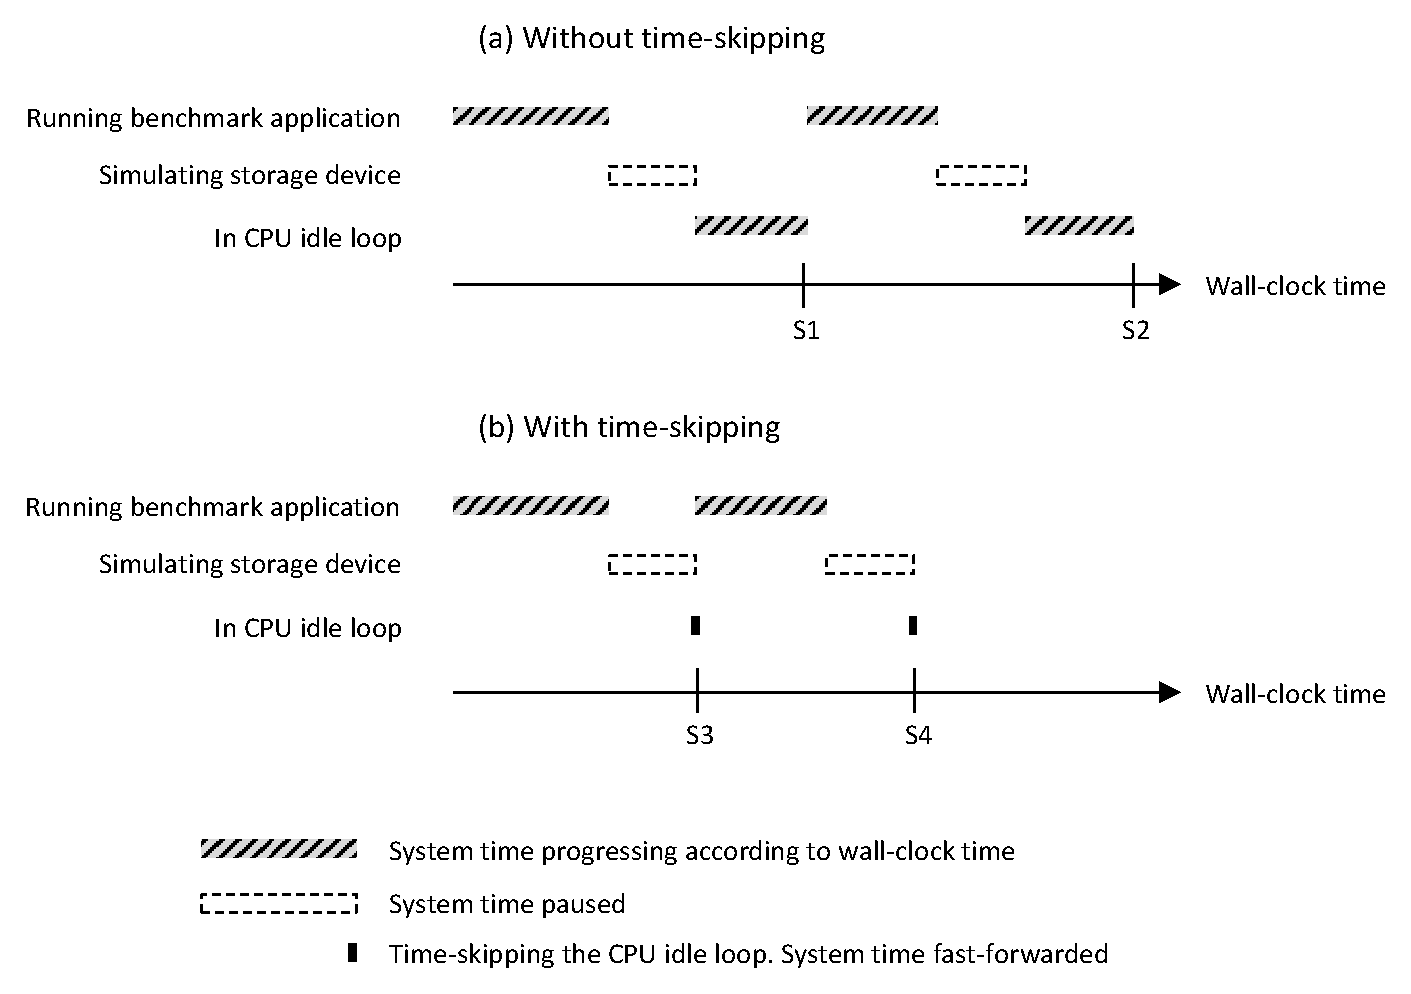
\includegraphics[width=1\textwidth]{figures/ch3-time-skipping.pdf}
	\caption{\label{fig:ch3-time-skipping}Example operation of CPU idle loop time-skipping.}
\end{figure}

An example operation of the CPU idle loop time-skipping feature is illustrated in Figure~\ref{fig:ch3-time-skipping}. This example illustrates a benchmark application submitting two I/O requests to the simulated storage device. The state of the OS is paused as soon as the I/O request is received by the simulated storage device. The work of simulating the I/O response is done while the OS is in the paused state (i.e., while the system time is paused). After the servicing time for the I/O response is determined, the OS will enter the idle mode to wait for the corresponding servicing time to pass by before it will receive the I/O response from the simulated storage device. With the CPU idle loop time-skipping feature, the actual waiting time in the CPU idle loop can be skipped. The OS state at S1 will be the same as the OS state at S3, and the OS state at S2 will be the same as the OS state at S4.

%Discuss the possible problem of "driver timeout".

When fast-forwarding the system time of the OS, special attention needs to be paid to device drivers that interact with real-world device entities. Some device drivers will have timeout mechanisms for detecting device errors. To maintain proper operation, theses timeout values will need to be adjusted accordingly taking into account the speedup ratio of the system time.

%\chapter{Previous Work}
\label{ch:4}

The key concept of the proposed co-simulation methodology is to control the execution state of the OS and make the OS to observe a virtual system time that is not hardwired to the real world clock. In the work of Gupta~\cite{Gupta:2006}, they proposed a technique called \textit{time dilation} to make the OS to observe a passage of time that is a constant time slower than the real-time clock. From the OS’s perspective, the physical resources in the external world will appear to be faster than their original speeds. For example, if the passage of time observed by the OS is slowed down by 10 times, then data arriving from a network interface at a physical rate of 1Gbps would appear to the OS as arriving at 10Gbps. They have demonstrated that \textit{time dilation} is an effective method for emulating network interfaces of different speeds to the OS for end-to-end system behavior experimentations. 

Although the proposed storage device emulator also makes the OS to observe a passage of system time that is different than the real-time clock, the goal and mechanisms are different from those of \textit{time dilation}:

\begin{itemize}
	\item  In \textit{time dilation}, the passage of system time is only slowed down by a constant factor but will never be stopped. In other words, the OS is always executing continuously. In contrast, in our proposed OS state pausing approach, the execution of the OS will be paused as necessary whenever the storage device emulator is busy processing the I/O requests. The goal of \textit{time dilation} is to trick the OS into believing that the external resources are faster than what they actually are. On the other hand, the goal of OS state pausing is to temporarily freeze the execution of the OS so that the storage device emulator can spend unlimited amount of time on processing the I/O requests.
	
	\item The slowing down of the passage of time in \textit{time dilation} is achieved by reducing the frequency that the timer interrupts are delivered to the OS and also by appropriately scaling down the hardware time counter that is used by the OS. For example, to slow down the passage of time observed by the OS by 10 times, the timer interrupt frequency is reduced by 10 times and the hardware time counter is also scaled down by 10 times. In comparison, pausing the state of the OS requires stopping the hardware time counter and preventing the CPU from doing any work for the OS.
	
	\item The design of the proposed storage device emulator can be extended with \textit{time dilation}. In the proposed emulator design, the OS can either be in the paused state or in the running state. When in the running state, it is possible to apply \textit{time dilation} so that the OS will observe that it is running on a CPU which is faster than the CPU of the target system. However, in order to keep our focus, we do not apply \textit{time dilation} to the proposed storage device emulator in this article.
\end{itemize}

Proper evaluation of storage subsystems is not an easy task. Traeger et al.~\cite{Traeger:2008} have proposed a set of guidelines for proper storage subsystem performance evaluations.
% TODO: Summarize the guide lines here.
Using the guidelines as the evaluation criteria, they have surveyed 415 file system and storage benchmarks from a selection of conference papers between the year 1999 and 2007. The selected benchmarks are all conducted on real machine environments. They have found that most benchmarks are flawed and could give the readers wrong impressions on the real performance of the storage subsystems under test and even lead to incorrect design conclusions. From the guidelines, it can be clearly seen that it is important that the system-level behaviors are taken into account when performing storage subsystem evaluation.

In the work of Ganger and Patt~\cite{Ganger:1998}, they have constructed abstract system-level model that contains necessary host system component modules with appropriate details for generating workloads for benchmarking storage subsystems. System-level traces, instead of I/O traces, are recorded on real system and played back using the abstract system-level model for generating workloads to drive the storage subsystem module.

Instead of using purely abstract models for system-level simulation, Thekkath~\cite{Thekkath:1994} incorporated real file system code into the simulation system. In his approach, I/O traces are gathered on real systems and are used to drive the real file system code in the simulation process for generating I/O requests.

An alternative to using abstract system-level models for performing storage subsystem evaluations is to use complete machine simulation. The SimOS environment~\cite{Rosenblum:1995} \cite{Witchel:1996} \cite{Rosenblum:1997} is a complete machine simulator which can simulate the hardware of an SGI machine in enough detail to run the Irix OS. SimOS supports switching among a number of hardware component models which are different in terms of modeling detail and accuracy. The less detailed models can run faster and can be used to boot and position the system into a state at which interesting workloads will begin. The simulation can then switch to use a more accurate model for detailed profiling. Griffin et al. [2000] has integrated a MEMS-based storage device simulator into the SimOS environment for studying the performance and characteristics of MEMS-based storage devices. Although complete machine simulation does allow the actual OS and real applications to be run on the simulated machine hardware, it can run much slower than the real system. Furthermore, building and maintaining accurate complete machine simulation models could take substantial amount effort.

Timing-accurate storage emulation has been explored in detail by \cite{Griffin:2002}. Memulator allows researchers to explore with nonexistent storage devices and take end-to-end measurements in full-system contexts. Memulator can use either the memory of the local machine or a networked machine as the backing storage for the emulated disk. Their work gives support that storage device emulation is an effective method for studying the overall system performance with simulated virtual storage devices. In their remote emulation setup, the emulator is executed on a standalone computer and connected to the target system over the SCSI interface. The DiskSim simulator~\cite{Bucy:2008} is used for simulating the service times of the Seagate Cheetah X15 hard disk drive. Experimental results show that the benchmark results measured with the emulated storage device are close to the results measured with the real storage device.

In the work of Maghraoui et al.~\cite{ElMaghraoui:2010}, a local emulation type storage device emulator is developed to emulate flash based SSD for the AIX OS. The emulator is implemented as a dynamic loadable kernel module and appears to the OS as a disk device. A chunk of system memory is pined for use as the backing storage, and high resolution nanosecond granularity timers are used for simulating the delays of the I/O operations. Lee et al.~\cite{Lee:2012} have proposed another local emulation type SSD emulator. The target platform is the Linux OS and it uses a user mode SSD simulation engine for calculating the latencies for the I/O requests. The backing storage used can be either the system memory or some other external DRAM-based storage devices.

David~\cite{Agrawal:2012} is another local emulation type storage device emulator which is mostly concerned about the required backing storage size for emulating large storage devices. The main idea of David is to reduce the data that needs to be saved to the backing storage so that larger storage devices can be emulated using less storage space. The key idea is that for certain types of benchmark workloads, the actual content in the file system files can be omitted and only file system metadata needs to be persisted onto the backing storage. By not persisting the actual content in the files, David is able to reduce the storage size requirements by orders of magnitude. David has been demonstrated to work with the ext3 and the btrfs file systems, and in theory, it can be extended to work with other types of file systems.

VSSIM~\cite{Yoo:2013} is a virtual machine (VM) based SSD simulator which makes emulated SSD devices available to the VM. The emulated SSD device appears to the VM as a storage device connected to the IDE interface. VSSIM runs in real-time and allows the user to measure both the host performance and the SSD behavior under various design choices. The design of VSSIM can conceptually be classified as similar to the remote emulation design. The difference is that the target machine that the emulated storage device is ``connected'' to is a VM, and therefore VSSIM does not need to emulate the actual electrical signals of the IDE interface.

Finally, Canon et al.~\cite{Canon:1980} extended the standard virtual machine (VM) environment to include virtual time emulation. In contrast to the conventional VM environment, in which the real time of day (RTOD) clock is observed by the VM, the modified VM environment makes the VM to observe a virtual time of day (VTOD) clock. The VTOD clock progresses as program instructions are executed on the virtual CPU of the VM. In the modified VM environment, the system performance is evaluated against the VTOD clock. The VM environment proposed by Canon et al. can be viewed as analogous to the SimOS environment configured with the direct execution model, in which the machine instructions are executed on the native CPU whenever possible and that the internal architecture of the CPU is not modeled.


\chapter{A Full-System Co-Simulator for Storage Subsystem Evaluation}
%TODO: A Full-System Co-Simulation Environment for Storage Subsystem Evaluation
\label{ch:5}

In this chapter, an OS-based full-system co-simulation environment based on the proposed virtual storage device and real computer system co-simulation methodology is described. The proposed full-system co-simulator can be used for performing storage subsystem evaluations in full-system contexts. Specifically, the virtual storage device can be simulated together with the entire OS and benchmark applications so that it can be evaluated using realistic real-world workloads and system-level measurement metrics.

The OS chosen for the implementation of the proposed full-system co-simulator is the Ubuntu Linux version 11.0 with kernel version 3.0.0-19~\cite{Ubuntu:2013}. The CPU architecture is the Intel x86 architecture. The concepts and modifications described in this chapter should also be applicable to other OS's and CPU architectures. Figure~\ref{fig:ch5-full-system-simulator} illustrates the overall architecture of the proposed full-system co-simulator. There are two key parts to the design of the proposed full-system co-simulator. The first part is related to the modifications made to the task scheduling and timekeeping infrastructures of the Linux kernel for controlling the state of the OS. These modifications are related to the ability for co-simulating the virtual storage device and physical computer system in the discrete-time domain. The related modules are shown in the gray blocks in Figure~\ref{fig:ch5-full-system-simulator} and are discussed in section~\ref{sec:managing-linux-OS-state} and \ref{sec:controlling-current-system-time}. The second part is related to the emulating of the virtual storage device to the OS. The related modules are shown in the white blocks with solid lines and are discussed in section~\ref{sec:storage-device-simulation-module} and \ref{sec:direct-backing-storage}.

\begin{figure}[htpb]
	\centering
	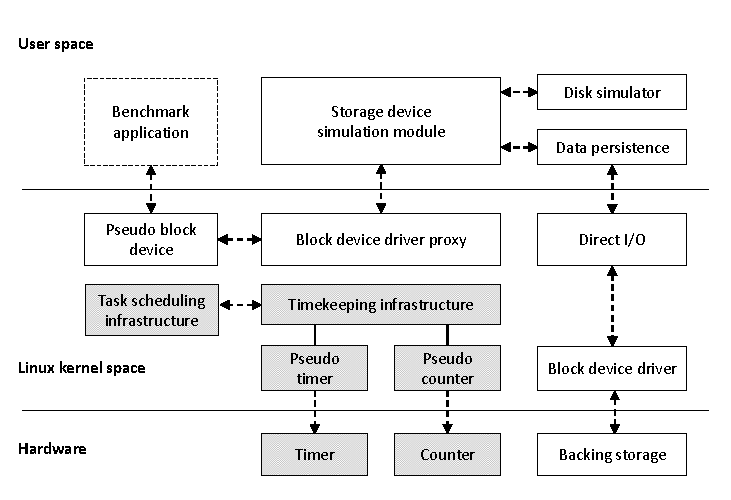
\includegraphics[width=1\textwidth]{figures/ch5-full-system-simulator.pdf}
	\caption{\label{fig:ch5-full-system-simulator}Overview of the proposed full-system co-simulator.}
\end{figure}

\section{Controlling the State of the Linux Operating System}
\label{sec:managing-linux-OS-state}

The state of the Linux OS can be viewed as the combined state of the user space processes, the kernel space threads, and the current system time. Here, the user space processes and the kernel space threads are collectively called the normal OS processes. In comparison, the processes responsible for simulating the storage device are called the simulator processes. The state of the Linux OS can be paused by blocking all normal OS processes from executing on the CPU and stopping the advancement of the hardware timer and counters.

The task scheduler of the Linux kernel is modified so that the normal OS processes can be distinguished from the simulator processes. Whenever the simulator processes are executing, the Linux OS will be put into the paused state. Because of the pausing made to the OS state, the behaviors of the normal processes, and therefore the system-level behaviors that are of interest, will not be affected by the simulator processes.

\begin{figure}[htpb]
	\centering
	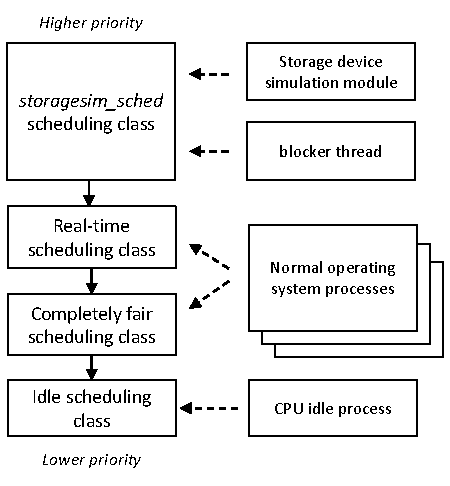
\includegraphics[width=0.6\textwidth]{figures/ch5-scheduling-classes.pdf}
	\caption{\label{fig:ch5-scheduling-classes}Scheduling classes in the Linux task scheduling infrastructure.}
\end{figure}

As illustrated in Figure~\ref{fig:ch5-scheduling-classes}, the task scheduler of the Linux OS is made up of several scheduling classes (\textit{struct sched_class}, defined in \textit{include/linux/sched.h}). In the stock Linux kernel, the normal OS processes can belong to either the real-time (RT) scheduling class (\textit{rt_sched_class}, implemented in \textit{kernel/sched_fair.c}) or the completely fair scheduling (CFS) class (\textit{fair_sched_class}, implemented in \textit{kernel/sched_fair.c})~\cite{Bovet:2005}, \cite{Love:2010}. The RT scheduling class has higher priority than the CFS class. That is, processes in the RT scheduling class always get to run before the processes in the CFS class.

In the proposed full-system co-simulator, a special \textit{storagesim_sched} scheduling class is implemented and given the highest priority in the task scheduler. The simulator processes, such as the processes that are responsible for simulating the storage device, are registered under the \textit{storagesim_sched} scheduling class. Therefore, whenever the storage device simulation module has to handle the simulation of the virtual storage device, it will be scheduled immediately and blocks all normal processes from running. Furthermore, when the task scheduler selects a process from the \textit{storagesim_sched} scheduling class, the task scheduler will know that the process is one of the simulator processes and will make a request to the modified timekeeping infrastructure to pause the current system time. The preventing of the normal OS processes from running and the pausing of the current system time effectively puts the Linux OS into the paused mode. To bring the OS base to the normal running state when the normal OS processes are selected again for running, the current system time will be set to progress normally according to the wall-clock time.

Because the normal OS processes are scheduled according to the same scheduling algorithms in the unmodified Linux kernel (i.e., by the RT and the CFS scheduling classes), the multi-tasking behavior of the Linux OS is preserved in the proposed full-system co-simulator.

When the simulator process releases itself form using the CPU, it is possible that it still requires that the OS is kept in the paused mode for some indefinite amount of time. For example, when the storage device simulation module needs to read some data from the backing storage to prepare for an I/O response, it will be put into the I/O wait state when waiting for the response from the backing storage. During this wait period on the backing storage, the state of the Linux OS should still remain in the paused mode even if there is no simulator process needs to use the CPU. That is, the Linux OS cannot be put back to the running mode yet. Otherwise, when the storage device simulation module finally receives the actual data from the backing storage and is ready to reply the I/O response to the OS, the OS state might have already have advanced past the intended system time at which the I/O response should be replied at.

To handle the need for keeping the OS in the paused mode while waiting for the data from the backing storage, a kernel space ``blocker thread'' is introduced. The blocker thread is a kernel thread that runs an infinite idle loop and is registered as the lowest priority thread in the \textit{storagesim_sched} scheduling class. The blocker thread can be enabled or disabled by the simulator processes through a system call. The storage device simulation module will enable the blocker thread before issuing requests to the backing storage and disables it after the responses are received.

\section{Controlling the Current System Time}
\label{sec:controlling-current-system-time}

The timekeeping infrastructure of the Linux kernel is responsible for providing two services to the system: (1) Provisioning of the current system time, and (2) Provisioning of a timer service which can be used to schedule callback events in future time points.

Historically, the Linux kernel tracks system time and schedules timer callback events using a periodic timer tick. The internal kernel value \textit{jiffies} records the number of timer ticks since the system is powered on and is incremented at each timer interrupt. Depending on the kernel configuration, the frequency of the timer interrupt is typically between 100Hz to 1000Hz. That is, the resolution of \textit{jiffies} is typically between 1\si{\milli\second} and 10\si{\milli\second}. Due to the coarse resolution of \textit{jiffies}, the proposed full-system co-simulator cannot rely on it to represent the Linux OS state for discrete event simulation. For example, if the Linux OS is put into the running mode at time \textit{t} and runs for 0.5\si{\milli\second} before it makes an I/O request to the virtual storage device, then when switching to the paused mode, the state of the Linux OS should be recorded to be at time \textit{t}+0.5\si{\milli\second}. However, if \textit{jiffies} with resolution of 1\si{\milli\second} is used for representing the current system time of the Linux OS state, it is not possible to represent the OS state at exactly \textit{t}+0.5\si{\milli\second}. Only representing the discrete state of the Linux OS at the \textit{jiffies} granularity (i.e., down to 1\si{\milli\second}) is insufficient for the purpose of storage subsystem evaluation.

A na\"{\i}ve solution would be to increase the resolution of the \textit{jiffies} to a higher resolution. However, the problem with this approach is that it will significantly change the original behavior of the Linux OS. For example, having the \textit{jiffies} at the 1\si{\micro\second} resolution would mean that the hardware timer will need to be interrupting the Linux OS at one million times per second. This will cause the interrupts to consume a lot of additional CPU cycles. Furthermore, even at 1\si{\micro\second} resolution, it could still be too coarse for representing the state of the Linux OS.

\begin{figure}[htpb]
	\centering
	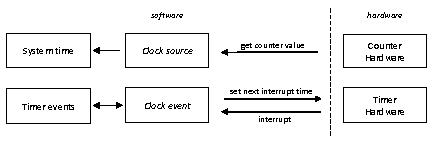
\includegraphics[width=0.95\textwidth]{figures/ch5-clocksource-clockevent.pdf}
	\caption[The \textit{clock source} and \textit{clock event} devices.]{\label{fig:ch5-clocksource-clockevent}The \textit{clock source} and \textit{clock event} devices in the Linux timekeeping infrastructure.}
\end{figure}

Between kernel version 2.6.19 and 2.6.21, a new timekeeping infrastructure was introduced to the Linux kernel~\cite{Stultz:2005}, \cite{GleixnerNiehaus:2006}, \cite{GleixnerMolnar:2006}, \cite{Gleixner:2007}, \cite{Kerrisk:2012}. As illustrated in Figure~\ref{fig:ch5-clocksource-clockevent}, the new timekeeping infrastructure is composed of \textit{clock source} and \textit{clock event} devices. To be able to control the system time in a finer granularity, the proposed full-system co-simulator requires that the Linux kernel is configured to use this new timekeeping infrastructure.

The \textit{clock source} device, defined in \textit{/kernel/time/clocksource.h}, is used to provide the current system time to the timekeeping infrastructure. It utilizes a monotonically increasing hardware counter in the system for measuring elapsed time. When the current time value is needed, the \textit{clock source} device reads the hardware counter and translates the counter value into current system time. The unit of the current system time is in nanoseconds. Depending on the hardware configuration, there could be many available hardware counters in a system. The timekeeping infrastructure will select the most suitable hardware counter to be used as the \textit{clock source} device. The chosen device It is usually the hardware counter with the highest resolution. On the testing platform of the proposed full-system co-simulator, the hardware counter selected is the Time Stamp Counter (TSC)~\cite{Intel:1997}, \cite{wiki:TSC}.

As illustrated in Figure~\ref{fig:ch5-full-system-simulator}, in the proposed full-system co-simulator, the hardware counter selected by the timekeeping infrastructure will be wrapped by a pseudo software counter. Therefore, by controlling the value of the pseudo counter, the current system time perceived by the Linux OS can be controlled. Furthermore, because the TSC counter selected in the test platform has a resolution of a single CPU clock cycle, the current system time part of the Linux OS state can be precisely captured.

The \textit{clock event} device, defined in \textit{/kernel/time/clockevents.h}, is used for providing timer callback service. The timer events in the Linux kernel are sorted in a red-block tree data structure. The most recent timer event will always be programed to the \textit{clock event} device. When programed, the \textit{clock event} device will set the timer hardware in the system. The timer hardware utilized in the testing platform is the Local Advanced Programmable Interrupt Controller (LAPIC) timer. As illustrated in Figure~\ref{fig:ch5-full-system-simulator}, the selected hardware timer is wrapped by a pseudo software timer. Through the pseudo software timer, the full-system co-simulator can know the next time point that a timer event will happen. This knowledge is used by the time-skipping feature to fast-forward the simulation time when the CPU enters the idle loop. The time-skipping feature is discussed in section~\ref{sec:time-skipping}.

By intercepting and controlling the values that the pseudo counter and the pseudo timer provide to the upper layers of the timekeeping infrastructure, the timekeeping infrastructure is modified to support the following operations:

\begin{itemize}
	\item Normal operation when in running mode --- When the Linux OS is in the running mode, the value of the pseudo counter is incremented at the same rate as the real TSC counter. The pseudo counter only needs to be synchronized with the TSC counter when it is being referenced. To the Linux OS, the system time will be progressing at the real-world clock speed. In addition, when timer event is programmed to the pseudo timer, the pseudo timer will set the corresponding timer value the real LAPIC timer.
	
	\item Switch from running mode to paused mode --- When Linux needs to be switched from running mode to paused mode, two steps are performed for proper mode switch operation: (1) Disables the hardware timer and records the remaining time in the pseudo timer. For example, if the pseudo timer is set with an expiration time of 10\si{\milli\second} when in the running mode, and after 4\si{\milli\second} the Linux OS is switched to the paused mode, then the timekeeping infrastructure should remember that there is still 6\si{\milli\second} remaining in the pseudo timer. (2) Pauses the hardware counter so that the value of the pseudo clock will remain constant. This effectively pauses the current system time.
	
	\item Fast-forward the current system time --- When Linux enters the idle mode and the time-skipping feature is enabled, the timekeeping infrastructure will fast-forward the current system to a future time point as determined by the remaining time in the pseudo timer. The fast-forward operation is performed by adding the remaining time value to the pseudo clock. After the system time is fast-forwarded, Linux can be put back to the running mode immediately and the simulation continues.
	
	\item Switch from paused mode to running mode --- After the simulation process releases the CPU, Linux will be put back to the running mode from the paused mode. The hardware counter is enabled so that the system time will be progressing at real-world clock speed. For proper mode switch operation, if there is a remaining countdown value in the pseudo timer when the OS is being switched to the paused mode, the remaining time in the pseudo timer is programmed to the hardware timer.
\end{itemize}

\section{Block Device Driver Proxy}
\label{sec:storage-device-simulation-module}

The Linux kernel has a well-defined block device driver programming interface for supporting block devices~\cite{Corbet:2005}, \cite{Venkateswaran:2008}. The simulated virtual storage device in the proposed full-system co-simulator is made available to the Linux kernel by emulating a virtual storage device over the standard block device driver programming interface. The virtual storage device can be used by the reset of the Linux OS just like a real storage device. Normally, the block device drivers are implemented in the kernel space. However, because existing disk model simulators, such as DiskSim~\cite{Bucy:2008} and Vesper~\cite{DeRosa:2006}, are user space programs, the proposed full-system co-simulator implements a block device driver proxy so that the simulation of the virtual storage device can be carried out in the user space. This technique is similar to the idea adopted by the Filesystem in Userspace (FUSE) project~\cite{wiki:FUSE}. The relations between the pseudo block device, the block device driver proxy, and the virtual storage device simulation module are illustrated in Figure~\ref{fig:ch5-full-system-simulator}. The storage device simulation module uses the APIs provided by the block device driver proxy to be able to simulate the pseudo block devices to the Linux kernel in user space. The APIs provided by the block device driver proxy are described in Table~\ref{tab:II} .  

\begin{table}[htpb]%
	\renewcommand{\arraystretch}{1.3}
	\centering
	\caption{APIs provided by the block device driver proxy}\label{tab:II}
	\noindent\begin{tabularx}{\textwidth}{|p{3.5cm}|X|}
	\hline
	\centering\bfseries API & \centering\bfseries\arraybackslash Description \\ \hline
	\textit{register_disk} & The \textit{register_disk} system call is used for registering a new pseudo block device to the Linux kernel. The main parameter is the capacity of the pseudo block device. The return value is a handle to the pseudo block device. \\ \hline
	
	\textit{get_request} & Retrieve the pending I/O requests for the corresponding pseudo block device. \\ \hline
	
	\textit{sleep_on_disk} & The \textit{sleep_on_disk} system call implements a high resolution sleep function that will return control to the user space program under two conditions: (1) When the specified sleep time expires, or (2) when a new I/O request is submitted to the corresponding pseudo block device. \\ \hline
	
	\textit{respond_request} & The \textit{respond_request} system call is used for returning the I/O responses to the block device driver proxy. Internally, the block device driver proxy uses the \textit{blk_complete_request} kernel function to notify the Linux kernel about the completion of an I/O request. \\ \hline
	\end{tabularx}
\end{table}


\section{Direct Backing Storage Access}
\label{sec:direct-backing-storage}

When the Linux kernel is under memory pressure, the memory manager will try to reclaim system memories by flushing some memory pages to the block device. If the memory pages are flushed to the simulated storage device, then it is important that the processing path for the I/O write request does not allocate any more memory from the Linux kernel. Otherwise, it can lead to system deadlocks because there might not be any more allocatable memories left in the Linux kernel. Therefore, care must be taken to make sure that the storage device simulation module does not allocate any additional memory once it completes initialization and starts to provide block device access to the Linux kernel. That is, the storage device simulation module must allocate all of its required memories at initialization time and the entire program needs to be pinned to the physical memory.

The storage device simulation module needs to persist the actual data of the simulated storage device to the real storage devices.  When a sector of the simulated storage device is written, the actual data needs to be saved to the backing storage, and when a sector of the simulated storage device is read, the actual data needs to be retrieved from the backing storage. As illustrated in Figure~\ref{fig:ch5-direct-backing-storage}, the VFS layer in the Linux kernel might need to allocate more memory during its operation. Therefore, to avoid system deadlocks, the storage device simulation module must not access the backing storage through the VFS layer. The proposed full-system co-simulator has implemented a direct backing storage access mechanism that allows the storage device simulation module to persist data the real storage devices without going through the VFS layer.

\begin{figure}[htpb]
	\centering
	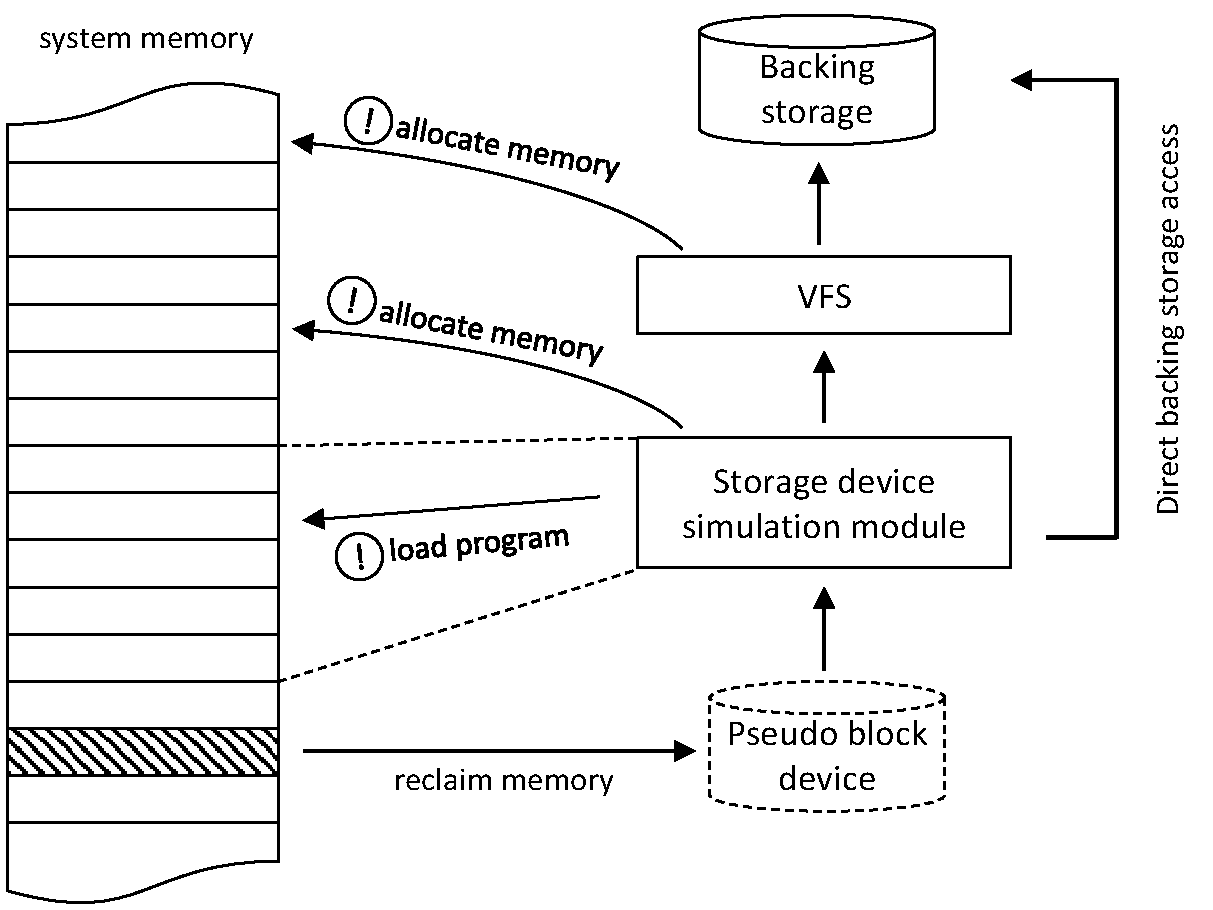
\includegraphics[width=0.8\textwidth]{figures/ch5-direct-backing-storage.pdf}
	\caption{\label{fig:ch5-direct-backing-storage}Avoid allocating memory in the storage device simulation path.}
\end{figure}


\section{Integration with Third-Party Disk Simulators}
\label{sec:disk-simulator-integration}

The storage device simulation module relies on disk simulators to calculate the I/O service timings and simulate the behaviors of the target storage device. The storage device simulation module has three main functions:
\begin{enumerate*}[label=(\arabic*)]
	\item \label{ch5-third-party-one} Calculate the service times of the I/O requests using a disk model, 
	\item \label{ch5-third-party-two} Save and retrieve the actual data of the I/O requests to and from the backing storage, and
	\item \label{ch5-third-party-three} Submit the I/O responses to the Linux kernel at the corresponding service times as calculated in \ref{ch5-third-party-one}.
\end{enumerate*}

The storage device simulation module provides a well-defined API for integration with third-party disk simulators. When third-party disk simulators are integrated into the proposed full-system co-simulator, they can be used by the storage device simulation module to calculate the service timings in \ref{ch5-third-party-one}. Because the designs of \ref{ch5-third-party-two} and \ref{ch5-third-party-three} are decoupled with \ref{ch5-third-party-one}, no additional modifications will be needed if a different disk simulator is used for calculating the service timings of the I/O requests.

\begin{figure}[htpb!]
	\centering
	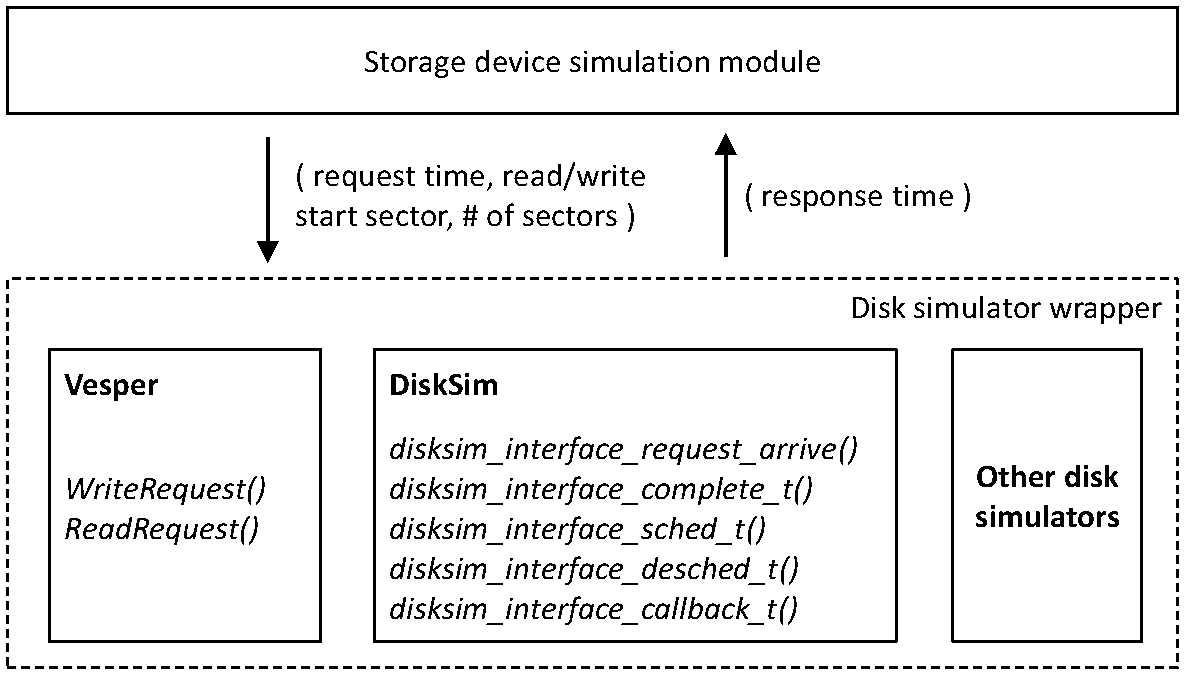
\includegraphics[width=0.85\textwidth]{figures/ch5-disk-simulator-integration.pdf}
	\caption{\label{fig:ch5-disk-simulator-integration}Interface for integration with third-party disk simulators.}
\end{figure}

As illustrated in Figure~\ref{fig:ch5-disk-simulator-integration}, the interface for integrating third-party disk simulators with the storage device simulation module is simple. For each I/O request, the storage device simulation module will provide four pieces of information to the disk simulator: request time, request type (read or write), start sector, and number of sectors. The responsibility of the disk simulator is to calculate the response timings of the I/O requests and return them to the storage device simulation module. If the APIs provided by the third-party disk simulators are different from the aforementioned interface, wrappers can be used for adapting to the provided APIs.

The proposed full-system co-simulator is integrated with two disk simulators: Vesper~\cite{DeRosa:2006} and DiskSim~\cite{Bucy:2008}. The Vesper disk simulator was originally released as part of the Nachos instructional OS~\cite{Christopher:1993}. The source code of Vesper is separated from Nachos~\cite{Pearson:2007} and made operational as a standalone library. A wrapper is developed to make Vesper compatible with the storage device simulation module's API interface. In this case, the wrapper simply uses one of the internal \textit{WriteReqeust} or \textit{ReadRequest} API of Vesper to compute the service timings for the incoming I/O requests.

The second disk simulator that is supported is the DiskSim simulator. DiskSim is itself implemented as a discrete event simulator. It provides APIs for injecting and receiving events from its internal simulation loop. When an I/O request is to be processed, the wrapper injects the I/O request into DiskSim using the \textit{disksim_interface_request_arrive} function. It then simulates DiskSim until the I/O completion time is reported from DiskSim through the \textit{disksim_interface_complete_t} function callback.

\section{Experimental Results}
\label{sec:ch5-experimental-results}
The target platform used for evaluating the proposed full-system co-simulator is a computer equipped with a 3.1 GHz Intel Core i5-3210M processor and 16 GB of DDR3 memory. A 240 GB Intel 520 series SSD is used as the backing storage. The storage device simulation module in the proposed full-system co-simulator supports two different kinds of disk simulators: DiskSim and Vesper. It also supports two types of backing storages: SSD and RAM.

DiskSim provides more detailed simulation of the behaviors of the disk device at the cost of higher computation complexity. Vesper is a faster disk simulator that provides adequate realism for system-level performance evaluations. In some system-level performance studies, very detailed modeling of a specific disk device is not needed. For example, when designing the I/O scheduling algorithm in an OS for general rotational disks, using a disk simulator that captures the essential characteristics of the rotational mechanical disk devices will be sufficient as the I/O scheduling algorithm will be used with different disk devices. In this case, only simulating the essential characteristics of mechanical disk devices such as disk head track switching time, rotational delay, and buffering could be adequate. Vesper can be chosen as the disk simulator when conducting this kind of system-level performance evaluations.

Because the system time of the Linux OS is controlled by the simulation kernel and is no longer linked the real-world clock time, it cannot be used for measuring the elapsed time of the simulation. A special system call is added to the Linux kernel for getting the real wall clock time from the real hardware counter. On the test computer, the Time Stamp Counter (TSC), which is available on all modern x86 processors, is used for measuring the elapsed wall clock time. The TSC counter is incremented every CPU clock cycle. With the CPU running at 3.1GHz on the test computer, the TSC counter has a resolution of approximately 0.3\si{\nano\second}.

For the testing workloads, vdbench (version 5.02)~\cite{Vdbench:2013} is used for generating 18 kinds of I/O access profiles. Each workload profile has three attributes: access type, read/write type, and request size. The access type can be ``random'' or ``mixed.'' The read/write type can be ``read,'' ``write,'' or ``read-write.'' The request size can be ``small,'' ``uniform,'' or ``large.'' A random workload has zero probability of local accesses or sequential accesses; request starting locations are uniformly distributed across the entire storage capacity of the tested hard disk drive. A mixed workload has 80\% probability of random accesses and 20\% of sequential accesses. A read workload is composed of all read accesses, a write workload is composed of all write accesses, and a read-write workload is composed of 50\% read accesses and 50\% write accesses. A small workload is composed of 8-sector (4KB) requests, a large workload uses 256-sector (128KB) requests, and a uniform workload has uniformly distributed request sizes in intervals of 4KB over the range [4KB, 128KB]. All workload profiles continuously generate I/O requests at the maximal speed at which can be sustained by the simulated storage device for 3 minutes.

\subsection{Timing Accuracy of the Simulated Storage Device}

In the work of timing-accurate storage emulation by Griffin et al.~\cite{Griffin:2002}, to evaluate how closely the storage emulator comes to perfect timing-accurate emulation, they have compared the per-request I/O service times observed by the OS to the per-request service times as reported by the DiskSim disk simulator. If the differences between the OS observed I/O service times and the times reported by DiskSim is small, then it means that the performance characteristics of the emulated storage device as perceived by the OS is close to the intended target. From their experimental results, it had been shown that the performance prediction accuracy is good when over 99\% of all emulated I/O responses have less than 2\% error. 

In the proposed full-system co-simulator, when an I/O request is received by the storage device simulation module, it will use the disk simulator (e.g., DiskSim or Vesper) to calculate the intended response time for the I/O request. The storage device simulation module will then register a timer to wait for the arrival of the intended response time. When the timer expires, the storage device simulation module will wake up and reply the I/O response to the Linux kernel. Due to things such as OS state pausing overhead and process context switch latencies, the time point at which the Linux kernel receives the I/O response might not be exactly the same as the intended response time as calculated by the disk simulator. For example, if the disk simulator calculates that an I/O request should be completed at time $t$ and that the Linux kernel actually receives the I/O response at time $t + \Delta t$, then the timing error value of the I/O response is said to be $\Delta t$. The percent timing error of the I/O response is $(\Delta t / t) \times 100\%$. 

The timing error of the simulated storage device in the proposed full-system co-simulator is measured. The storage device simulation module is configured with the Vesper disk simulator and using SSD as the backing storage. The target storage device modeled is the IBM 08K0383 36G hard disk drive. Each of the 18 workload profiles generated by vdbench is submitted to the simulated storage device. The timing errors for a total of 468,964 I/O responses are measured. Figure~\ref{fig:ch5-fig-15a} shows the distribution of the timing error values. Over 99.995\% of the I/O responses measured have a timing error value of less than 20\si{\micro\second}. Figure~\ref{fig:ch5-fig-15b} shows the distribution of the percent timing errors. The percent timing error of an I/O response is calculated by dividing the timing error value by the service time of the corresponding I/O request as computed by the Vesper disk simulator. Over 99.98\% of all the I/O responses measured have less than 0.5\% timing error.

\begin{figure}[htpb]
	\centering
	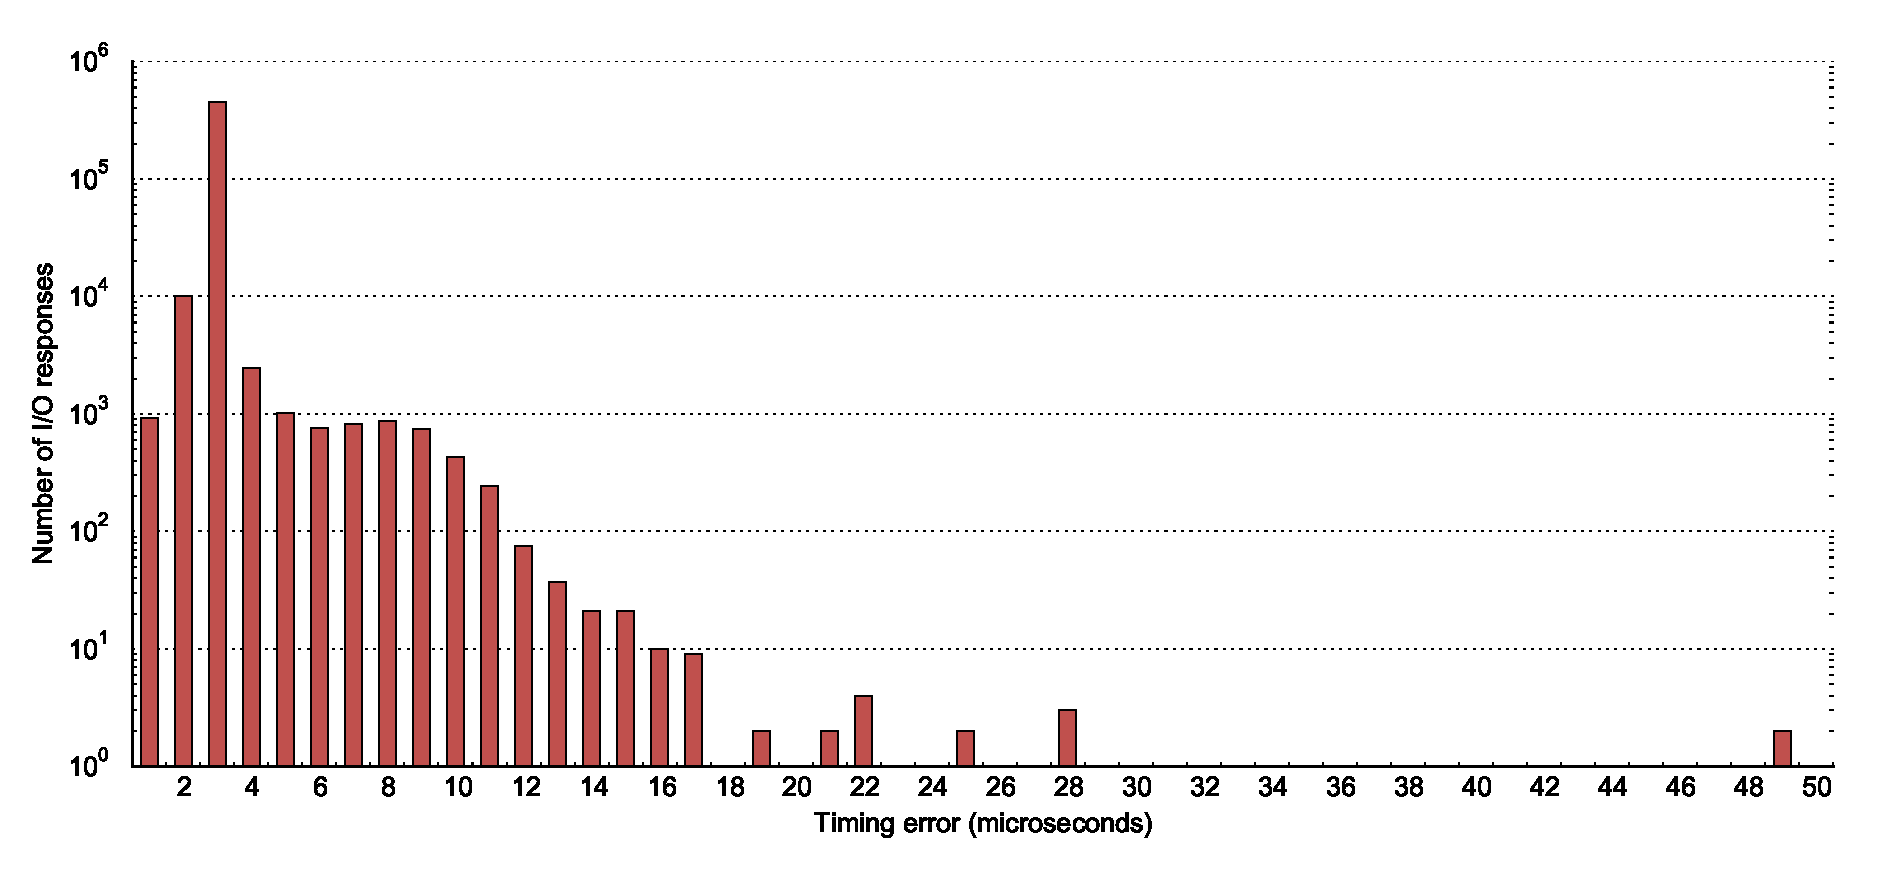
\includegraphics[width=\textwidth]{figures/ch5-fig-15a.pdf}
	\caption{\label{fig:ch5-fig-15a}Timing error of the simulated storage device.}
\end{figure}

\begin{figure}[htpb]
	\centering
	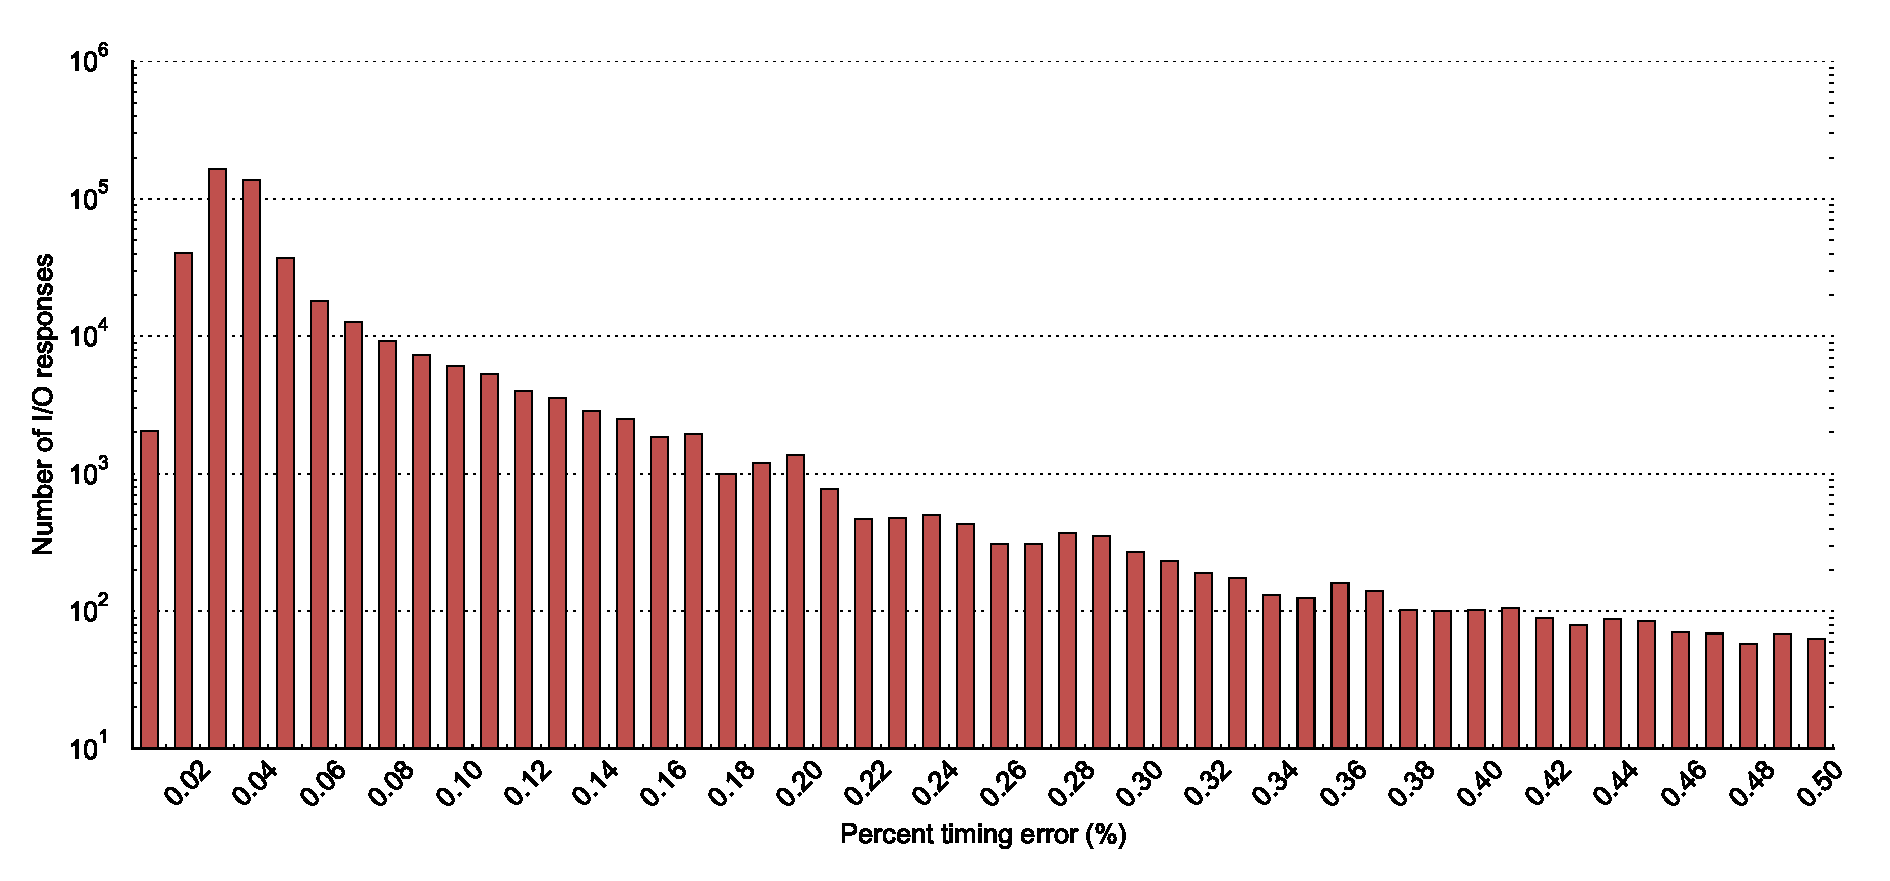
\includegraphics[width=\textwidth]{figures/ch5-fig-15b.pdf}
	\caption{\label{fig:ch5-fig-15b}Percent timing error of the simulated storage device.}
\end{figure}


\subsection{Simulation Speed}
\label{sec:simulation-performance}

The speed at which the proposed full-system co-simulator can carry out the simulation process depends on many factors. The three most relevant factors are summarized as follows:

\begin{itemize}
	\item The performance of the simulate storage device that is modeled --- The faster the simulated storage device is, the more I/O requests can be handled during the same system time span, and thus the more simulation work needs to be carried out. For example, when the storage subsystem is fully stressed, simulating a system equipped with a 15k RPM disk will be slower than simulating the same system equipped with a 5.4k RPM disk.
	
	\item The performance of the storage device simulation module --- The faster the storage device simulation module can compute the I/O request timings and handle the actual data of the simulated storage device, the faster the simulation process will be. Therefore, using a simple disk model simulator such as Vesper will be faster than using a more complex disk model simulator such as DiskSim. Similarly, using RAM as the backing storage will be faster than using a storage device as the backing storage.
	
	\item The I/O access pattern of the benchmark workload --- Different benchmark workload will generate I/O requests of different intensity. A light weight benchmark workload will leave the co-simulator more time in the CPU idle loop. This means that there will be more opportunity for time-skipping the CPU idle loop and thus leads to faster simulation speed.
\end{itemize}

Table~\ref{tab:DiskSim-and-SSD-result} to Table~\ref{tab:Vesper-and-RAM-speed} show the experimental results. The meaning of the columns in the tables are explained as follows. The ``Simulation result'' columns show the metrics measured on the Linux OS, which are respect to the virtual time system. ``I/O per second'' and ``Bandwidth'' are the benchmark results from the vdbench program. ``Elapsed system time'' is the time span that vdbench is running and generating workloads toward the simulated storage device. It is measured using the \textit{time} command of the Linux OS. The values in the ``vdbench CPU time'' column are also measured using the \textit{time} command, showing the user and system CPU time used by vdbench. The values in the ``Simulation speed'' columns are measured using the real TSC clock. ``Elapsed wall clock time'' is the total amount of time that the proposed full-system co-simulator used for carrying out the simulation. The ``In paused mode'' column shows how much time the Linux OS is put into the ``paused'' mode. The ``DiskSim busy'' or the ``Vesper busy'' column shows how much time when the OS in the ``paused'' mode is consumed by DiskSim or Vesper. The ``Backing storage busy'' column shows how much time during the simulation is spent waiting for the backing storage. The final column shows the speedup that the proposed full-system co-simulator has achieved. The values in this column equal to the ratio between the values of ``Elapsed system time'' and ``Elapsed wall clock time''.

In the first set of experiments, DiskSim is configured as the disk simulator and SSD is used as the backing storage. The virtual storage device being simulated is a Seagate Cheetah 15k.5 147GB hard disk drive. It has a spindle speed of 15K and an average seek time of less than 4\si{\milli\second}. The raw disk device is benchmarked. The device is opened with the O_DIRECT flag to bypass the system buffer caches. The experimental results are shown in Table~\ref{tab:DiskSim-and-SSD-result} and Table~\ref{tab:DiskSim-and-SSD-speed}. For each simulation run, the system is rebooted to prevent interferences from the previous executions. Observations from the first set of experimental results are summarized as follows.

\begin{itemize}
	\item The proposed full-system co-simulator has achieved faster-than-real-time simulation of a complete system running the Linux OS with DiskSim simulating a modern server grade hard disk drive. The speedup achieved in the experimental setup is between 1.07$\times$ to 2.27$\times$.
	
	\item Because vdbench is an I/O bound benchmark application, not much CPU time is consumed by vdbench. During the simulated time span, the Linux OS is relatively idle and can be time skipped. Note that when the values in ``Time used by vdbench'' is subtracted from  the values in ``Simulated timespan'', the resulting numbers are very close to the total simulation time that can be time skipped.
	
	\item The majority of the simulation time is consumed by DiskSim. Over 97\% of the time when the OS is in the paused mode is used by DiskSim.
	
	\item For each test, the summation of the value in the ``DiskSim computation time'' column and the value in the ``Backing storage operation time'' column can be longer than the total time spent in the paused mode. This is because the design of the storage simulation module allows backing storage to work in parallel while the request timings are being calculated.
\end{itemize}

\begin{table}[htbp]%
\small
\begin{center}
\caption{Simulation results for DiskSim and SSD}\label{tab:DiskSim-and-SSD-result}
\hspace*{-2cm}
\noindent\begin{tabular}{lcS[table-format=2.2]cc}
	\toprule
	& \multicolumn{4}{c}{Simulation result} \\
	\cmidrule(lr){2-5}
	\parbox{3cm}{\centering Workload \\ profile} & \parbox{2cm}{\centering I/O per \\ second } & \parbox{2cm}{\centering Bandwidth \\ (MB/sec) } & \parbox{2cm}{\centering Elapsed \\ system time} & \parbox{3cm}{\centering vdbench CPU time\\ (user / sys)} \\
	
	\midrule
	
	random / read / small & 172.75 & 0.67 & 187.945 & 2.416 / 0.082 \\
	random / read / large &	140.74 & 17.59 & 187.305 & 2.444 / 0.960 \\
	random / read / uniform & 155.06 & 10.01 & 188.285 & 2.344 / 0.904 \\
	random / write / small & 171.51 & 0.67 & 187.495 & 2.540 / 0.900 \\
	random / write / large & 142.76 & 17.84 & 188.986 & 2.432 / 1.144 \\
	random / write / uniform & 156.09 & 10.07 & 187.574 & 2.760 / 0.872 \\
	random / read-write / small & 170.45 & 0.67 & 187.277 & 2.604 / 0.760 \\
	random / read-write / large & 140.15 & 17.52 & 188.050 & 2.468 / 1.032 \\
	random / read-write / uniform & 153.99 & 9.95 & 188.448 & 2.524 / 0.920 \\
	mixed / read / small & 243.19 & 0.95 & 189.274 & 2.344 / 1.040 \\
	mixed / read / large & 186.37 & 23.30 & 187.214 & 2.592 / 1.184 \\
	mixed / read / uniform & 211.22 & 13.67 & 187.741 & 2.540 / 1.120 \\
	mixed / write / small & 195.20 & 0.76 & 187.818 & 2.620 / 0.944 \\
	mixed / write / large & 160.27 & 20.03 & 190.912 & 2.556 / 1.188 \\
	mixed / write / uniform & 176.60 & 11.43 & 187.470 & 2.708 / 1.164 \\
	mixed / read-write / small & 210.87 & 0.82 & 187.173 & 2.648 / 0.908 \\
	mixed / read-write / large & 169.69 & 21.21 & 188.417 & 2.584 / 1.196 \\
	mixed / read-write / uniform & 188.50 & 12.23 & 187.386 & 2.676 / 1.080 \\

	\bottomrule
\end{tabular}
\hspace*{-2cm}
\end{center}

	Remarks: The full-system co-simulator is configured to use DiskSim as the disk simulator and SSD as the backing storage. The target storage device modeled is the 147GB Seagate Cheetah 15k.5 hard disk drive. Units are in seconds unless otherwise specified.
\end{table}%


\begin{table}[htbp]%
	\small
	\begin{center}
	\caption{Simulation speed for DiskSim and SSD}\label{tab:DiskSim-and-SSD-speed}
	\hspace*{-2cm}
	\noindent\begin{tabular}{
			l
			S[table-format=3.3]
			S[table-format=3.3]
			r
			S[table-format=3.3]
			c
			}
		\toprule
		& \multicolumn{5}{c}{Simulation speed} \\
		\cmidrule(lr){2-6}
		\parbox{3cm}{\centering Workload \\ profile} & \parbox{1.8cm}{\centering Elapsed \\ wall clock \\ time } & \parbox{1.2cm}{\centering In paused mode } & \parbox{3.2cm}{\centering DiskSim busy \\ (\% of paused mode)} & \parbox{1.2cm}{\centering Backing \\ storage \\ busy} & \parbox{1.5cm}{\centering Speedup \\ over \\ real-time}\\
		
		\midrule
		
		random / read / small & 82.659 & 78.746 & 77.246 (98.09\%) & 8.165 & 2.27$\times$ \\
		random / read / large &	140.425 & 136.388 & 134.363 (98.52\%) & 54.385 & 1.33$\times$ \\
		random / read / uniform & 116.217 & 112.315 & 110.462 (98.35\%) & 34.336 & 1.62$\times$ \\
		random / write / small & 79.065 & 74.878 & 73.410 (98.04\%) & 8.970 & 2.37$\times$ \\
		random / write / large & 145.042 & 140.651 & 138.142 (98.22\%) & 95.977 & 1.30$\times$ \\
		random / write / uniform & 115.682 & 111.270 & 109.209 (98.15\%) & 55.715 & 1.62$\times$ \\
		random / read-write / small & 79.163 & 75.071 & 73.747 (98.24\%) & 8.526 & 2.37$\times$ \\
		random / read-write / large & 141.414 & 137.181 & 135.054 (98.45\%) & 73.220 & 1.33$\times$ \\
		random / read-write / uniform & 116.484 & 112.294 & 110.444 (98.35\%) & 45.032 & 1.62$\times$ \\
		mixed / read / small & 86.378 & 82.221 & 80.369 (97.75\%) & 8.791 & 2.19$\times$ \\
		mixed / read / large & 165.248 & 160.728 & 158.086 (98.36\%) & 70.891 & 1.13$\times$ \\
		mixed / read / uniform & 129.401 & 124.952 & 122.480 (98.02\%) & 44.712 & 1.45$\times$ \\
		mixed / write / small & 119.795 & 115.464 & 113.844 (98.60\%) & 8.259 & 1.57$\times$ \\
		mixed / write / large & 178.576 & 173.933 & 171.083 (98.36\%) & 105.511 & 1.07$\times$ \\
		mixed / write / uniform & 153.308 & 148.564 & 146.152 (98.38\%) & 61.404 & 1.22$\times$ \\
		mixed / read-write / small & 106.426 & 102.080 & 100.494 (98.45\%) & 8.557 & 1.76$\times$ \\
		mixed / read-write / large & 171.517 & 166.913 & 164.363 (98.47\%) & 87.658 & 1.10$\times$ \\
		mixed / read-write / uniform & 141.370 & 136.767 & 134.503 (98.34\%) & 52.583 & 1.33$\times$ \\
		
		\bottomrule
	\end{tabular}
	\hspace*{-2cm}
	\end{center}

	Remarks: The full-system co-simulator is configured to use DiskSim as the disk simulator and SSD as the backing storage. The target storage device modeled is the 147GB Seagate Cheetah 15k.5 hard disk drive. Units are in seconds unless otherwise specified.
\end{table}%

In the second set of experiments, the proposed full-system co-simulator is configured to use Vesper as the disk simulator for calculating the service timings of the simulated storage device. The disk profile for the IBM 08K0383 36GB disk drive that comes with Vesper is used as the disk model for the simulated storage device. The IBM disk drive has a spindle speed of 10K and an average seek time of 4.7ms. The experimental results are shown in Table~\ref{tab:Vesper-and-SSD-result} and Table~\ref{tab:Vesper-and-SSD-speed}. Only the results for the ``mixed'' set of workload profiles are shown. Observations from the experimental results are summarized as follows.

\begin{itemize}
	\item Due to its simplicity, Vesper can calculate response timings for the simulated disk device much faster than DiskSim. Our measurements show that Vesper is up to three orders of magnitude faster than DiskSim.
	
	\item The backing storage operation is now dominating the time that the proposed full-system co-simulator spends in the paused mode. This leads to the motivation of the next set of experiments, which uses RAM as the backing storage to further speedup the simulation speed.
\end{itemize}

In the third set of experiments, the proposed full-system co-simulator uses Vesper for storage device timing calculation and RAM as the backing storage device. The IBM 08K0383 36GB disk drive is modeled. The experimental results are shown in Table~\ref{tab:Vesper-and-RAM-result} and Table~\ref{tab:Vesper-and-RAM-speed}. Only the results for the ``mixed'' set of workload profiles are shown. Some observations are:

\begin{itemize}
	\item Only a small fraction of time is now used by Vesper and the RAM-based backing storage. The proposed full-system co-simulator consistently achieves simulation speed of over 30$\times$ to 45$\times$ faster than real-time.
	
	\item Vdbench and other housekeeping tasks in the proposed full-system co-simulator are now accounting for over 90\% of the simulation time. By Amdahl's law, switching to an even faster disk timing simulator or backing storage will not have much gain for the simulation speed.
\end{itemize}

In summary, it has been demonstrated that the overhead of the proposed full-system co-simulator itself is lightweight and can achieve a full-system simulation speed of over 45 times faster than real-time in real world usage scenarios.

\begin{table}[htbp]%
	\small
	\begin{center}
	\caption{Simulation results for Vesper and SSD}\label{tab:Vesper-and-SSD-result}
	\hspace*{-2cm}
	\noindent\begin{tabular}{lS[table-format=3.2]ccc}
		\toprule
		& \multicolumn{4}{c}{Simulation result} \\
		\cmidrule(lr){2-5}
		\parbox{3cm}{\centering Workload \\ profile} & \parbox{2cm}{\centering I/O per \\ second } & \parbox{2cm}{\centering Bandwidth \\ (MB/sec) } & \parbox{2cm}{\centering Elapsed \\ system time} & \parbox{3cm}{\centering vdbench CPU time\\ (user / sys)} \\
		
		\midrule
		
		mixed / read / small & 147.28 & 0.58 & 186.337 & 2.364 / 0.652 \\
		mixed / read / large & 73.93 & 9.24 & 186.866 & 2.496 / 0.768 \\
		mixed / read / uniform & 97.96 & 6.33 & 187.867 & 2.452 / 0.688 \\
		mixed / write / small & 147.62 & 0.58 & 186.853 & 2.508 / 0.836 \\
		mixed / write / large & 73.79 & 9.22 & 187.346 & 2.504 / 0.944 \\
		mixed / write / uniform & 97.92 & 6.33 & 186.375 & 2.708 / 0.812 \\
		mixed / read-write / small & 146.84 & 0.57 & 185.886 & 2.428 / 0.744 \\
		mixed / read-write / large & 73.76 & 9.22 & 186.842 & 2.376 / 0.752 \\
		mixed / read-write / uniform & 97.91 & 6.37 & 186.874 & 2.528 / 0.796 \\
		
		\bottomrule
	\end{tabular}
	\hspace*{-2cm}
	\end{center}

	Remarks: The full-system co-simulator is configured to use Vesper as the disk simulator and SSD as the backing storage. The target device modeled is the 36GB IBM 08K0383 hard disk drive. Units are in seconds unless otherwise specified.
\end{table}%


\begin{table}[htbp]%
	\small
	\begin{center}
	\caption{Simulation speed for Vesper and SSD}\label{tab:Vesper-and-SSD-speed}
	\hspace*{-2cm}
	\noindent\begin{tabular}{
			l
			S[table-format=2.3]
			S[table-format=2.3]
			c
			S[table-format=2.3]
			S[table-format=2.2]
			}
		\toprule
		& \multicolumn{5}{c}{Simulation speed} \\
		\cmidrule(lr){2-6}
		\parbox{3cm}{\centering Workload \\ profile} & \parbox{1.8cm}{\centering Elapsed \\ wall clock \\ time } & \parbox{1.2cm}{\centering In paused mode } & \parbox{3.2cm}{\centering DiskSim busy \\ (\% of paused mode)} & \parbox{1.2cm}{\centering Backing \\ storage \\ busy} & \parbox{1.5cm}{\centering Speedup \\ over \\ real-time}\\
		
		\midrule
		
		mixed / read / small & 6.358 & 2.585 & 0.053 (2.04\%) & 3.819 & 29.31$\times$ \\
		mixed / read / large & 24.512 & 20.351 & 0.052 (0.25\%) & 22.071 & 7.62$\times$ \\
		mixed / read / uniform & 22.331 & 18.399 & 0.043 (0.23\%) & 19.932 & 8.41$\times$ \\
		mixed / write / small & 8.335 & 4.193 & 0.047 (1.12\%) & 5.552 & 22.42$\times$ \\
		mixed / write / large & 49.633 & 45.195 & 0.038 (0.08\%) & 47.577 & 3.77$\times$ \\
		mixed / write / uniform & 36.520 & 32.082 & 0.040 (0.12\%) & 34.131 & 5.10$\times$ \\
		mixed / read-write / small & 8.159 & 4.236 & 0.052 (1.23\%) & 5.515 & 22.78$\times$ \\
		mixed / read-write / large & 39.853 & 35.904 & 0.063 (0.18\%) & 37.872 & 4.69$\times$ \\
		mixed / read-write / uniform & 29.906 & 25.739 & 0.047 (0.18\%) & 27.499 & 6.25$\times$ \\
		
		\bottomrule
	\end{tabular}
	\hspace*{-2cm}
	\end{center}

	Remarks: The full-system co-simulator is configured to use Vesper as the disk simulator and SSD as the backing storage. The target device modeled is the 36GB IBM 08K0383 hard disk drive. Units are in seconds unless otherwise specified.
\end{table}%


% -------------------------- Vesper and RAM

\begin{table}[htbp]%
	\small
	\begin{center}
	\caption{Simulation results for Vesper and RAM}\label{tab:Vesper-and-RAM-result}
	\hspace*{-2cm}
	\noindent\begin{tabular}{lS[table-format=3.2]ccc}
		\toprule
		& \multicolumn{4}{c}{Simulation result} \\
		\cmidrule(lr){2-5}
		\parbox{3cm}{\centering Workload \\ profile} & \parbox{2cm}{\centering I/O per \\ second } & \parbox{2cm}{\centering Bandwidth \\ (MB/sec) } & \parbox{2cm}{\centering Elapsed \\ system time} & \parbox{3cm}{\centering vdbench CPU time\\ (user / sys)} \\
		
		\midrule
		
		mixed / read / small & 146.79 & 0.57 & 186.330 & 2.228 / 0.532 \\
		mixed / read / large & 73.83 & 9.23 & 188.614 & 2.420 / 0.504 \\
		mixed / read / uniform & 97.60 & 6.30 & 186.335 & 2.368 / 0.560 \\
		mixed / write / small & 147.51 & 0.58 & 186.387 & 2.668 / 0.540 \\
		mixed / write / large & 73.88 & 9.24 & 188.355 & 2.568 / 0.576 \\
		mixed / write / uniform & 97.95 & 6.33 & 187.117 & 2.852 / 0.540 \\
		mixed / read-write / small & 147.81 & 0.58 & 186.830 & 2.388 / 0.496 \\
		mixed / read-write / large & 73.82 & 9.23 & 188.101 & 2.640 / 0.572 \\
		mixed / read-write / uniform & 97.84 & 6.37 & 186.942 & 2.564 / 0.528 \\
		
		\bottomrule
	\end{tabular}
	\hspace*{-2cm}
	\end{center}

	Remarks: The full-system co-simulator is configured to use Vesper as the disk simulator and RAM as the backing storage. The target device modeled is the 36GB IBM 08K0383 hard disk drive. Units are in seconds unless otherwise specified.
\end{table}%


\begin{table}[htbp]%
	\small
	\begin{center}
	\caption{Simulation speed for Vesper and RAM}\label{tab:Vesper-and-RAM-speed}
	\hspace*{-2cm}
	\noindent\begin{tabular}{lccccc}
		\toprule
		& \multicolumn{5}{c}{Simulation speed} \\
		\cmidrule(lr){2-6}
		\parbox{3cm}{\centering Workload \\ profile} & \parbox{1.8cm}{\centering Elapsed \\ wall clock \\ time } & \parbox{1.2cm}{\centering In paused mode } & \parbox{3.2cm}{\centering DiskSim busy \\ (\% of paused mode)} & \parbox{1.2cm}{\centering Backing \\ storage \\ busy} & \parbox{1.5cm}{\centering Speedup \\ over \\ real-time}\\
		
		\midrule
		
		mixed / read / small & 4.052 & 0.689 & 0.036 (5.23\%) & 0.060 & 45.99$\times$ \\
		mixed / read / large & 5.117 & 1.618 & 0.033 (2.02\%) & 0.779 & 36.86$\times$ \\
		mixed / read / uniform & 4.784 & 1.283 & 0.034 (2.66\%) & 0.534 & 38.95$\times$ \\
		mixed / write / small & 4.562 & 0.727 & 0.035 (4.80\%) & 0.091 & 40.85$\times$ \\
		mixed / write / large & 5.941 & 2.188 & 0.031 (1.41\%) & 1.265 & 31.70$\times$ \\
		mixed / write / uniform & 5.691 & 1.683 & 0.033 (1.94\%) & 0.866 & 32.88$\times$ \\
		mixed / read-write / small & 4.214 & 0.719 & 0.036 (5.06\%) & 0.076 & 44.33$\times$ \\
		mixed / read-write / large & 5.712 & 1.900 & 0.033 (1.75\%) & 1.025 & 32.93$\times$ \\
		mixed / read-write / uniform & 5.254 & 1.500 & 0.034 (2.28\%) & 0.711 & 35.58$\times$\\
		
		\bottomrule
	\end{tabular} 
	\hspace*{-2cm}
	\end{center}

	Remarks: The full-system co-simulator is configured to use Vesper as the disk simulator and RAM as the backing storage. The target device modeled is the 36GB IBM 08K0383 hard disk drive. Units are in seconds unless otherwise specified.
\end{table}%


\section{Applications of the Proposed Full-System Co-Simulator}
\label{sec:use-case}

Using the proposed full-system co-simulator, virtually simulated storage device can be co-simulated with the real OS and application programs running on the physical computer hardware. This means that realistic real-world workloads and system-level measurement metrics can be used for predicting the performance of the simulated storage device. Sections~\ref{sec:ch5-faster-storage-devices} and \ref{sec:ch5-different-CPU-speeds} describes two example applications of the proposed full-system co-simulator.

\subsection{Studying the Effects of Having Faster Storage Devices}
\label{sec:ch5-faster-storage-devices}

The proposed full-system co-simulator can simulate storage devices that are faster and larger than the actual storage device available. This allows system-level effects to be studied assuming when storage devices of different speeds are available. During simulation, the state of the Linux OS can be paused to wait for the storage device simulation module to process the I/O requests. Therefore, the amount of time used for preparing the I/O responses will not affect the storage device's performance as perceived by the Linux OS. For example, even if the storage device simulation module uses 100\si{\milli\second} to prepare for the response of an I/O request that is supposed to have a service time of 10\si{\milli\second} to the OS, due to the OS state pausing technique, the Linux OS will still perceive that it only took the virtual storage device 10\si{\milli\second} for servicing the I/O request. This allows the proposed co-simulation environment to simulate storage devices that are faster than the real backing storage that is available.

When the real data of the simulated storage device is to be saved to the backing storage, a logical-to-physical mapping table is used for data block placement. Data block on the backing storage only needs to be allocated for sectors of the simulated storage device that have been written. This allocation-on-write design allows the proposed full-system co-simulator to simulate storage devices that are larger than the physical backing storage available on the simulation platform if not all sectors of the virtual storage device are written during the benchmarking.

In this section, the proposed full-system co-simulator is used for studying the effects of what faster storage devices will have on the target system. The setup of the target system is the same as described in section~\ref{sec:ch5-experimental-results}. Vesper is used as the disk simulator and the IBM 08K0383 36GB hard disk drive is used as the reference hard disk drive. The performance of the reference disk drive is used as the baseline for modeling other devices. For example, a disk drive marked with 10$\times$ speed should have 10 times the performance of the reference disk drive~\cite{Ruemmler:1994}. The disk configurations that have been studied range from 10$\times$ to 100$\times$ with a stepping of 10$\times$, and from 120$\times$ to 200$\times$ with a stepping of 20$\times$.

In Vesper, the total service time of an I/O request includes the seek time, the rotational delay, and the data transfer time. A simple track cache is also modeled. If the disk head has passed the requested sector after landing at the current track, the read request can be serviced directly by the track cache. The disk models used by Vesper are modeled by its rotational speed, seek times, and data transfer rates. The required seek times are different for different seek distances. The data transfer rates are different from inner to outer tracks. To model a disk drive with 10$\times$ speed in Vesper, the rotational speed and the data transfer rates of the reference disk drive is multiplied by 10, and the seek times are divided by 10.

The metric used for measuring the performance of the system is the amount of time that it takes to extract the bzip2-compressed source archive of the Linux kernel version 3.0.81 (linux-3.0.81.tar.bz2, 74MBytes)~\cite{Kernel:2013}. The archive is extracted to an ext3 file system. The file system is recreated for each test run. The file system is mounted with the sync option so that all writes to the file system are immediately written to the disk. Without setting the sync option, the benchmark could be testing against the caching performance of the system instead of the performance of the simulated disk drive. Two kinds of I/O schedulers are tested. They are the Completely Fair Queuing (CFQ) I/O scheduler~\cite{wiki:2013:CFQ} and the NOOP I/O scheduler~\cite{wiki:2015:NOOP}. The NOOP scheduler is a simple scheduler that only merges I/O requests but does not try to reorder them.

The simulation results for the NOOP scheduler are shown in Table~\ref{tab:ch5-NOOP-scheduler}. The results for the CFQ I/O scheduler are shown in Table~\ref{tab:ch5-CFQ-scheduler}. For both tables, the ``extraction time'' is the simulated extraction time predicted by the proposed full-system co-simulator. The ``ideal extraction time'' is the expected extraction time when assuming that the overall system performance scales linearly with the disk speed. Figure~\ref{fig:ch5-predicted-extraction-time} visualizes the results in the ``extraction time'' column. Figure~\ref{fig:ch5-speedup-over-reference} visualizes the results in the ``speedup over the reference disk'' column.

From ~\ref{fig:ch5-predicted-extraction-time}, observe that the actual extraction performance in both the NOOP and CFQ I/O schedulers are considerably lower than the ideal performance (based on na\"{\i}ve linear-speedup scaling). Looking at the CPU utilization column in Table~\ref{tab:ch5-NOOP-scheduler} and~\ref{tab:ch5-CFQ-scheduler}, notice that the CPU is becoming more utilized as the speed of the disk is raised. This explains the reason why the overall system performance does not scale linearly with the disk speeds. As the performance of the disk is increased, the extraction task is changing from an I/O-bound workload to a CPU-bound workload. Therefore, the CPU is becoming the dominating factor that limits the overall system performance.

Another observation is that when the CFQ scheduler is used, the extraction performance saturates more quickly than when the NOOP scheduler is used. A first guess might be that the CFQ scheduler is more CPU hungry than the NOOP scheduler. However, the CPU utilization rates have never reached over $56\%$ even in the case when the disk speed is $200\times$. Further investigation leads to the \textit{/sys\slash block\slash <device>\slash queue\slash iosched\slash slice_idle} % use \slash to allow line break
parameter of the CFQ scheduler. This parameter controls the amount of time that the CFQ scheduler will intentionally wait for future synchronous requests from different processes, even when there are pending asynchronous requests~\cite{Layton:2009}. The motivation of this design is to favor synchronous requests over asynchronous requests, and it can be viewed as a variant of the anticipatory scheduling algorithm~\cite{Iyer:2001}. The default value of the \textit{slic_idle} parameter is 8\si{\milli\second}. During this waiting period, the CFQ scheduler will not issue asynchronous requests to the storage device. However, in some cases such as when the underlying storage device is very fast, this design can have an adverse effect to the overall system performance.

In the test scenarios, changing the \textit{slice_idle} parameter to 0\si{\milli\second} makes the CFQ scheduler perform comparably to the NOOP scheduler. As we can see, when studying the performance of storage subsystem designs, this kind of complex interactions among the system components can be overlooked if detailed full-system models are not incorporated.

\begin{table}[htbp]%
	\small
	\centering
	\caption{Simulation results for the NOOP scheduler}\label{tab:ch5-NOOP-scheduler}
	\noindent\begin{tabular}{cSSSS}
		\toprule
		\parbox{2cm}{\centering Disk speed} & \parbox{3.5cm}{\centering Predicted extraction \\ time (seconds)} & \parbox{2.5cm}{\centering Speedup over \\ reference disk} & \parbox{3cm}{\centering Ideal extraction \\ time (seconds)} & \parbox{2.5cm}{\centering CPU utilization \\ (\% busy)} \\
		\midrule
		
		1$\times$ (reference) & 1821.706 & 1.00 & \multicolumn{1}{c}{-} & 2.99 \\
		10$\times$ & 214.287 & 8.50 & 1821.71 & 24.92 \\
		20$\times$ & 137.064 & 13.29 & 182.17 & 39.80 \\
		30$\times$ & 83.911 & 21.71 & 91.09 & 59.10 \\
		40$\times$ & 78.298 & 23.27 & 60.72 & 60.46 \\
		50$\times$ & 66.666 & 27.33 & 45.54 & 62.70 \\
		60$\times$ & 50.580 & 36.02 & 36.43 & 69.29 \\
		70$\times$ & 49.169 & 37.05 & 30.36 & 69.76 \\
		80$\times$ & 43.451 & 41.93 & 26.02 & 75.60 \\
		90$\times$ & 37.113 & 49.09 & 22.77 & 86.23 \\
		100$\times$ & 37.949 & 48.00 & 20.24 & 83.43 \\
		120$\times$ & 34.670 & 52.54 & 18.22 & 92.12 \\
		140$\times$ & 37.269 & 48.88 & 15.18 & 95.77 \\
		160$\times$ & 33.692 & 54.07 & 13.01 & 96.36 \\
		180$\times$ & 34.360 & 53.02 & 11.39 & 95.85 \\
		200$\times$ & 30.312 & 60.10 & 10.12 & 97.44 \\
		
		\bottomrule
	\end{tabular}
\end{table}%

\begin{table}[htbp]%
	\small
	\centering
		\caption{Simulation results for the CFQ scheduler}\label{tab:ch5-CFQ-scheduler}
	\noindent\begin{tabular}{cSSSS}
		\toprule
		\parbox{2cm}{\centering Disk speed} & \parbox{3.5cm}{\centering Predicted extraction \\ time (seconds)} & \parbox{2.5cm}{\centering Speedup over \\ reference disk} & \parbox{3cm}{\centering Ideal extraction \\ time (seconds)} & \parbox{2.5cm}{\centering CPU utilization \\ (\% busy)} \\
		\midrule
		
		1$\times$ (reference) & 1968.493 & 1.00 & \multicolumn{1}{c}{-} & 2.91 \\
		10$\times$ & 232.285 & 8.47 & 196.85 & 24.03 \\
		20$\times$ & 157.455 & 12.50 & 98.42 & 35.18 \\
		30$\times$ & 124.959 & 15.75 & 65.62 & 43.09 \\
		40$\times$ & 111.831 & 17.60 & 49.21 & 46.56 \\
		50$\times$ & 100.979 & 19.49 & 39.37 & 49.19 \\
		60$\times$ & 96.806 & 20.33 & 32.81 & 51.66 \\
		70$\times$ & 92.814 & 21.21 & 28.12 & 51.01 \\
		80$\times$ & 93.545 & 21.04 & 24.61 & 52.71 \\
		90$\times$ & 86.753 & 22.69 & 21.87 & 52.93 \\
		100$\times$ & 88.153 & 22.33 & 19.68 & 53.64 \\
		120$\times$ & 84.121 & 23.40 & 16.40 & 54.43 \\
		140$\times$ & 83.012 & 23.71 & 14.06 & 55.47 \\
		160$\times$ & 88.324 & 22.29 & 12.30 & 53.98 \\
		180$\times$ & 80.226 & 24.54 & 10.94 & 54.26 \\
		200$\times$ & 81.584 & 24.13 & 9.84 & 55.26 \\
		
		\bottomrule
	\end{tabular}
\end{table}%

\begin{figure}[htpb]
	\centering
	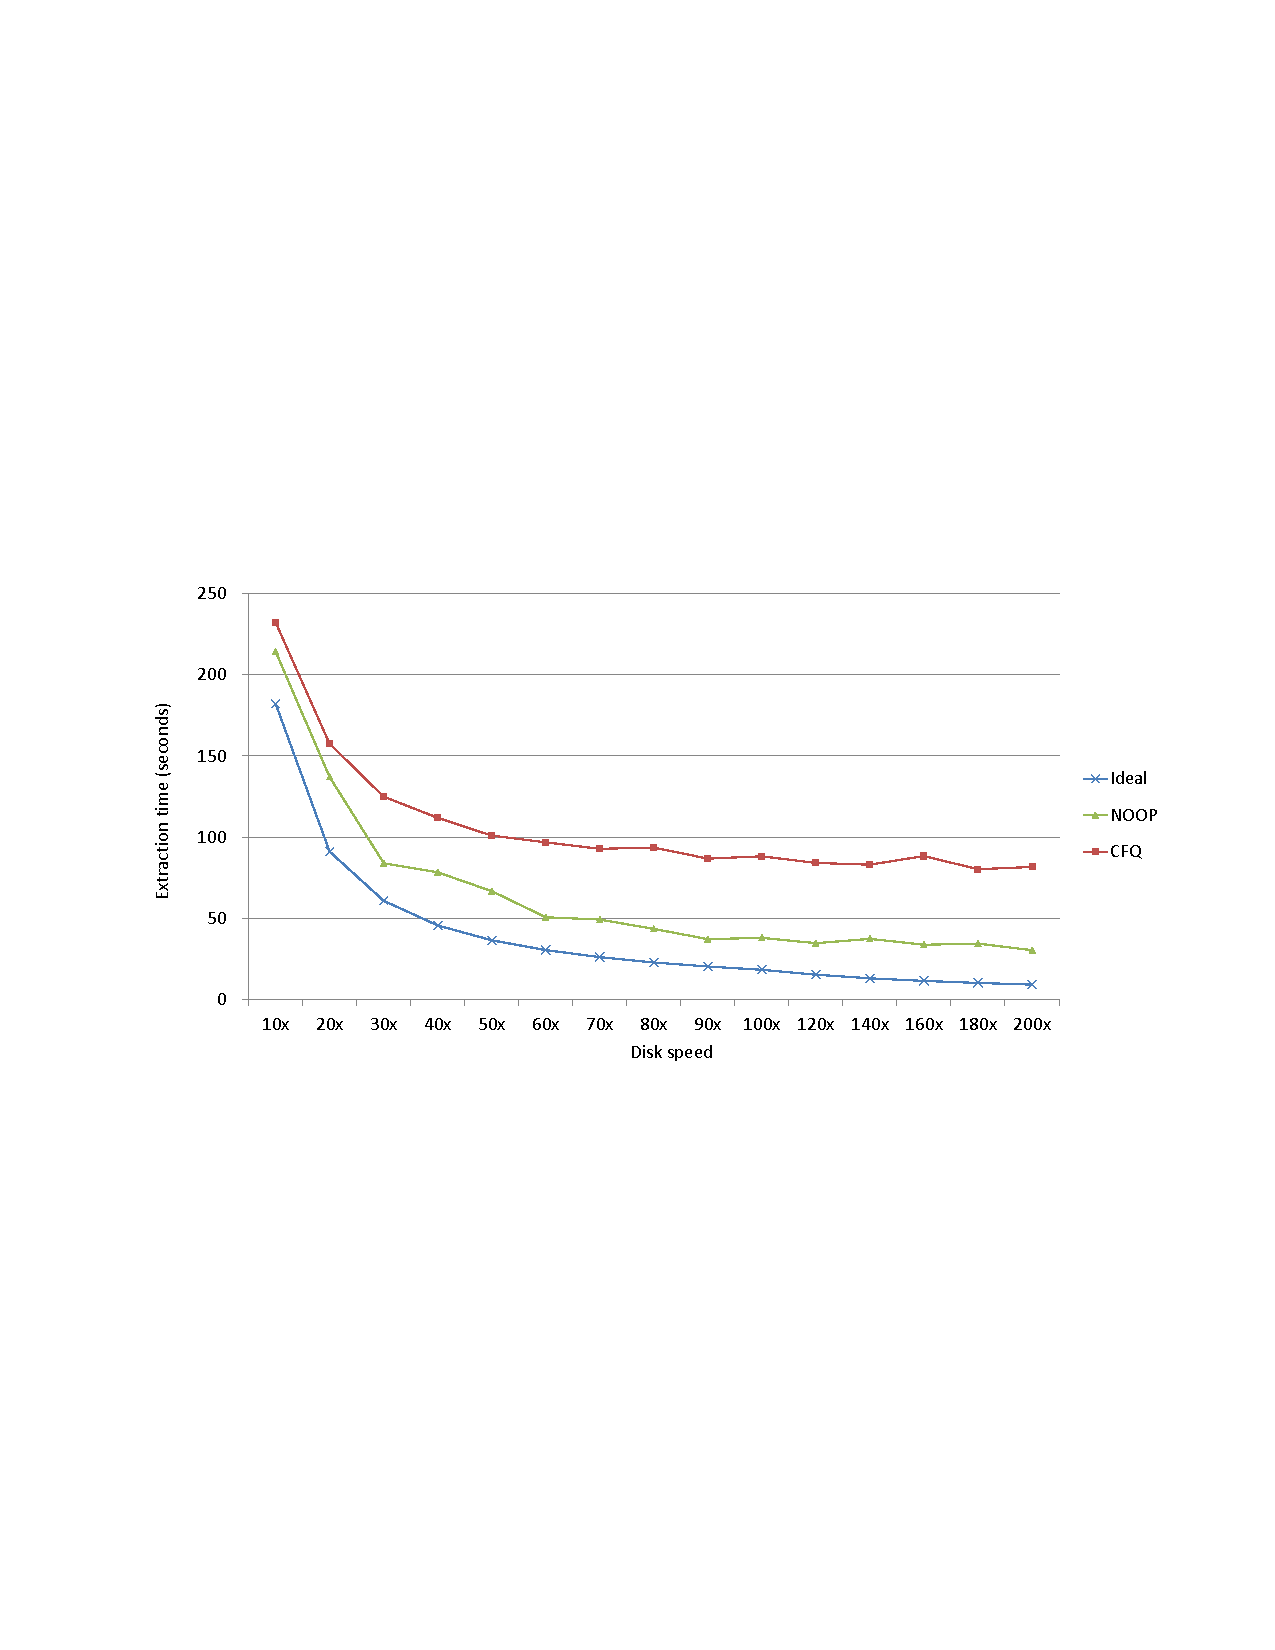
\includegraphics[trim=2cm 10cm 2cm 9.5cm, width=\textwidth]{figures/ch5-predicted-extraction-time.pdf}
	\caption{\label{fig:ch5-predicted-extraction-time}Predicted extraction time.}
\end{figure}

\begin{figure}[htpb]
	\centering
	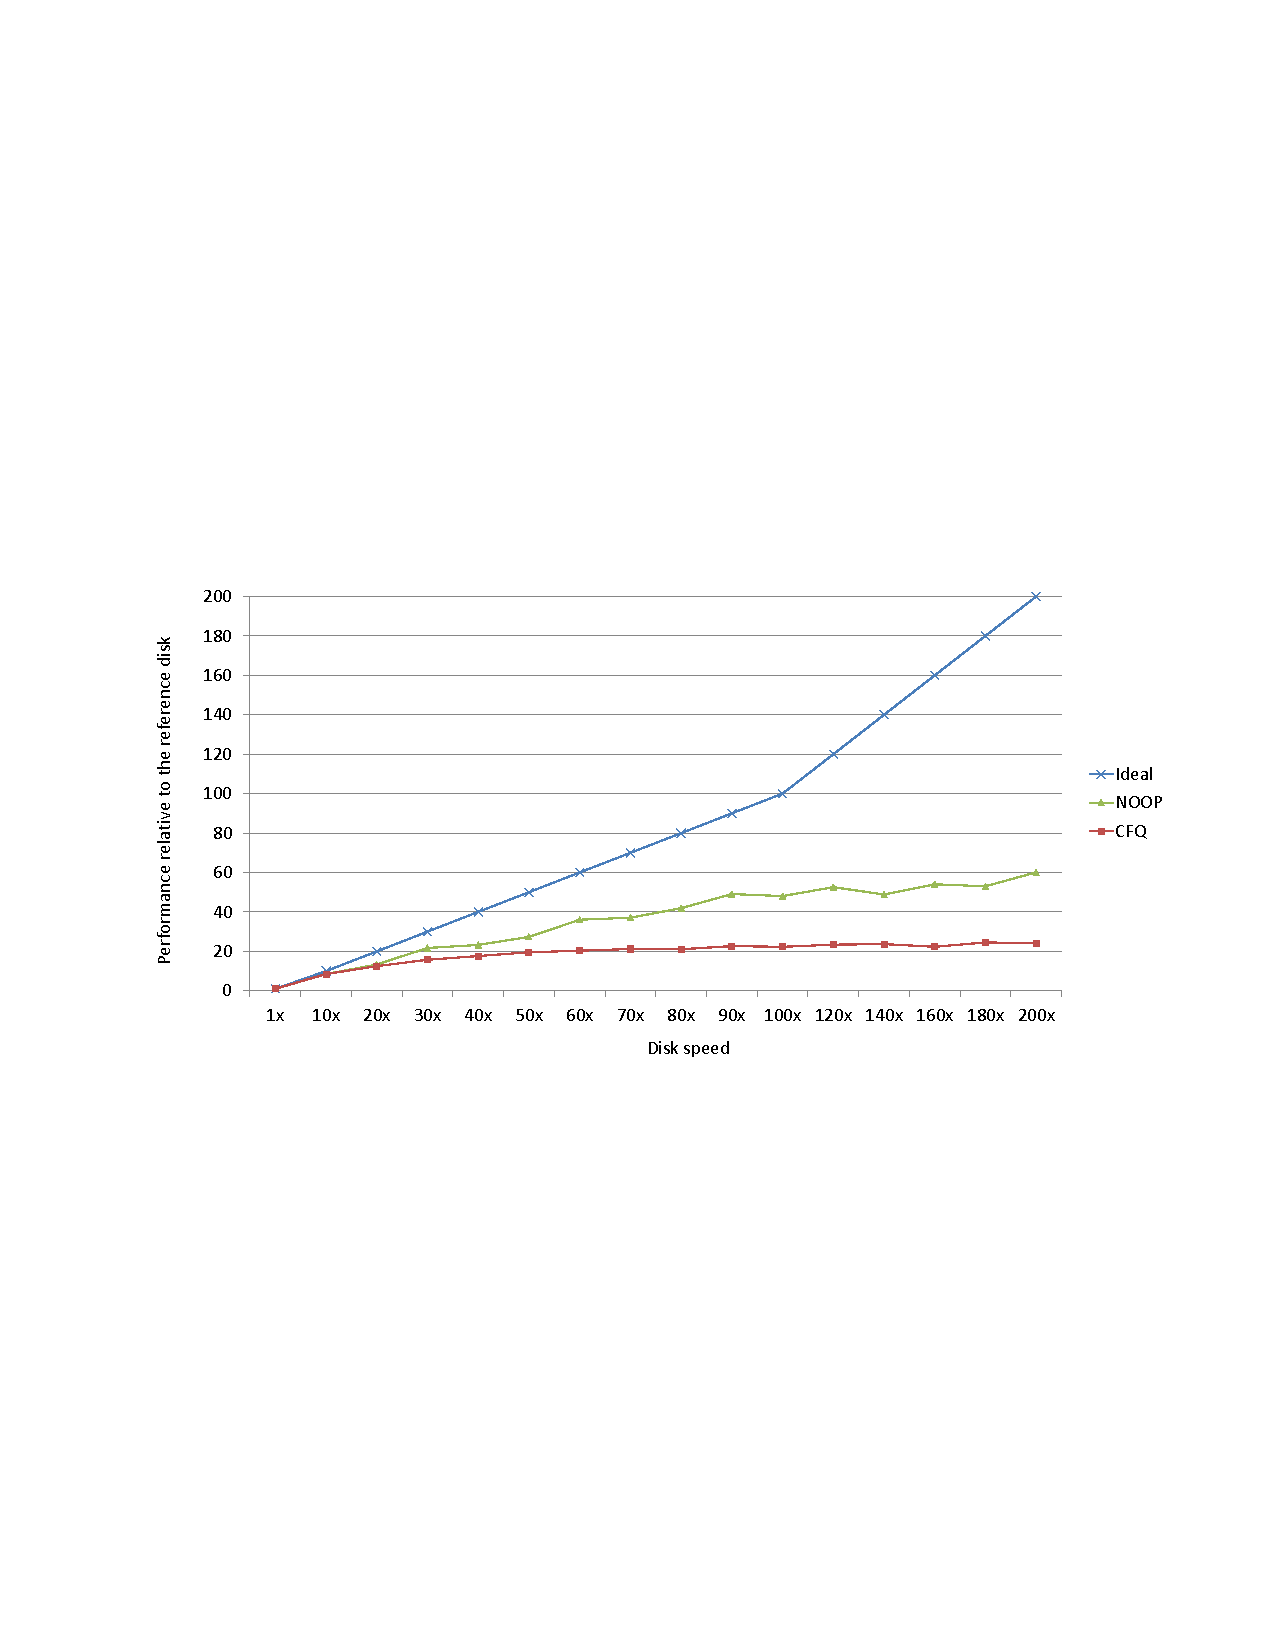
\includegraphics[trim=2cm 10cm 2cm 9.5cm, width=\textwidth]{figures/ch5-speedup-over-reference.pdf}
	\caption{\label{fig:ch5-speedup-over-reference}Speedups over the reference disk.}
\end{figure}


\subsection{Simulating Systems with Different CPU Speeds}
\label{sec:ch5-different-CPU-speeds}

By adjusting the rate at which the virtual system time advances, the proposed full-system co-simulator can trick the Linux OS into thinking that it is running on systems with different CPU speeds than the simulation host. For example, if the system time is advanced by one second for every two seconds that the Linux OS is in the running mode, then to the Linux OS the CPU would appear to be twice as fast as the real CPU that is on the simulation host. During the duration of the one second virtual system time, the CPU will have actually completed the amount of work that it can do in two seconds real-world clock time. With this capability of simulating systems with different CPU speeds, the proposed full-system co-simulator can be used for conducting sensitivity tests regarding what effects the CPU speeds will have to the overall system performance.

The common conception is that video encoding tasks are CPU-bound workloads. In the following use case, the ability of simulating systems with different CPU speeds is used to show that the performance of disk I/O subsystems could become the bottleneck for video encoding tasks. In the following experiments, the virtual storage device being simulated is the IBM 08K0383 36GB hard disk drive. The ext3 file system is used and is mounted with the sync option. The file system is recreated before each test run. The I/O scheduler used is the NOOP scheduler. The workload is generated by running 5 duplicates of the ffmpeg program (version 0.7.6) encoding the 300-frame standard MPEG CIF video test sequence Foreman~\cite{FFmpeg:2013}. The original RAW video is in YCBCR 4:2:0 format and it is encoded to the AVC/H.264 format. The CPU speeds simulated are ranged from 2$\times$ to 10$\times$ in 1$\times$ steps, and from 12$\times$ to 20$\times$ in 2$\times$ steps.

The simulation results are shown in Table~\ref{tab:ch5-encoding-time}. Figure~\ref{fig:ch5-encoding-time} depicts the same results in graphical form. Looking at the trend of the data points from the ``encoding time'' column, we can see that the overall system performance improvements are becoming saturated as the CPU speeds are reaching over seven times. From the disk utilization and CPU utilization data points, observe that the CPU utilization rates drop as the disk is becoming more utilized. In these simulations, the video encoding task has transformed from a CPU-bound workload into an I/O-bound workload as the CPU speed is raised. Such simulated scenarios are not entirely hypothetical since the computation tasks of video processing can be accelerated with the help of application specific acceleration logics~\cite{Wu:2009}, \cite{Wu:2015:ASAP}.


\begin{table}[htbp]%
	\small
	\centering
	\caption{Evaluation results for different CPU speeds}\label{tab:ch5-encoding-time}
	\noindent\begin{tabular}{ccccc}
		\toprule
		\parbox{2cm}{\centering CPU speed} & \parbox{3cm}{\centering Predicted encoding \\ time (seconds)} & \parbox{3cm}{\centering Speedup over \\ CPU with 1$\times$ speed} & \parbox{3cm}{\centering CPU utilization \\ (\% busy)} & \parbox{2.5cm}{\centering Disk utilization \\ (\% busy)} \\
		\midrule
		
		1$\times$ & 78.16 & 1.00 & 99.73 & 28.90 \\
		2$\times$ & 40.10 & 1.95 & 98.22 & 46.98 \\
		3$\times$ & 27.84 & 2.81 & 95.65 & 63.47 \\
		4$\times$ & 22.37 & 3.49 & 92.17 & 76.72 \\
		5$\times$ & 19.85 & 3.94 & 84.23 & 85.72 \\
		6$\times$ & 19.13 & 4.09 & 78.87 & 89.85 \\
		7$\times$ & 18.84 & 4.15 & 72.12 & 92.42 \\
		8$\times$ & 17.50 & 4.47 & 69.99 & 91.78 \\
		9$\times$ & 17.58 & 4.45 & 66.93 & 92.82 \\
		10$\times$ & 17.65 & 4.43 & 65.50 & 93.87 \\
		12$\times$ & 17.13 & 4.56 & 63.36 & 92.95 \\
		14$\times$ & 17.63 & 4.43 & 60.23 & 94.70 \\
		16$\times$ & 17.01 & 4.59 & 58.93 & 95.57 \\
		18$\times$ & 16.80 & 4.65 & 57.21 & 95.57 \\
		20$\times$ & 16.40 & 4.76 & 56.84 & 96.14 \\
		
		\bottomrule
	\end{tabular}
\end{table}%

\begin{figure}[htpb]
	\centering
	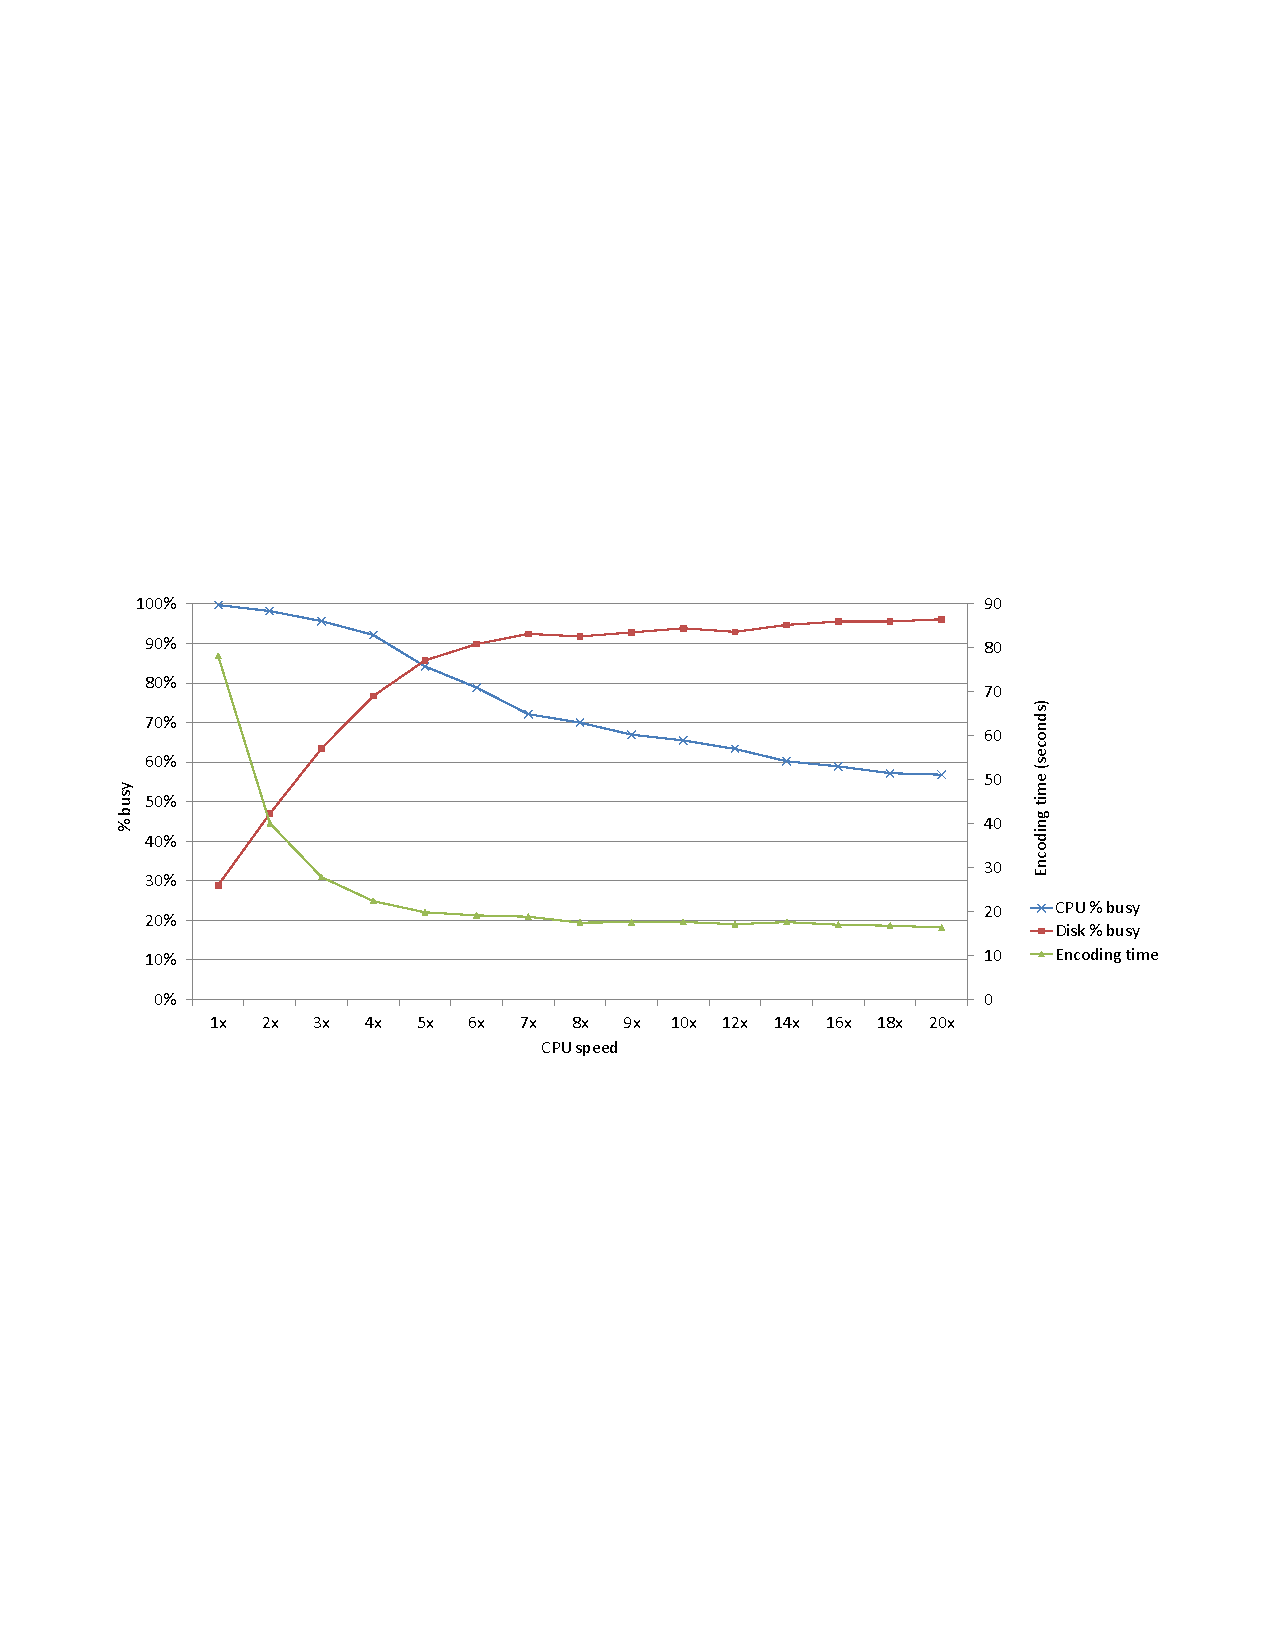
\includegraphics[trim=2cm 10cm 2cm 10cm, width=\textwidth]{figures/ch5-encoding-time.pdf}
	\caption{\label{fig:ch5-encoding-time}Video encoding performance on systems with different CPU speeds.}
\end{figure}


\chapter{A Storage Device Emulator for System Performance Evaluation}
\label{ch:6}

In this chapter, a storage device emulator based on the concept of OS state pausing is described~\cite{Wu:2015}. The full source code of the proposed storage device emulator is made available to the public domain\footnote{\url{http://www.cs.nctu.edu.tw/~cjtsai/research/nctusde}}. 

% motivation for this work. 
In the full-system simulator described in chapter~\ref{ch:5}, the work of simulating the virtual storage device is performed utilizing the target system's CPU. Due to the larger memory footprint for disk model simulation, the cache contents of the target system's CPU can be greatly altered each time the disk model is simulated. Altering the contents in the CPU cache can potentially change the performance behavior of a system. For example, if the system is performing a CPU intensive task while making a lot of accesses to the virtual storage device, the amount of time needed for completing the CPU intensive task can be affected due to cache content pollutions from the disk model simulator.

Since a storage subsystem design can be targeted for use in many systems with different performance characteristics, some amount of altering the performance of the target system while performing full-system co-simulation can be acceptable for the purpose of evaluating storage subsystem designs. However, for the purpose of predicting the performance of a specific target system when difference storage devices are available, we would like the performance characteristics of the target system to remain unaffected as much as possible.

To minimize the disturbance to the cache contents of the target system's CPU, the proposed storage device emulator described in this chapter offloads the work of storage device emulation to an external computer. An overview of the proposed storage device emulator is illustrated in Figure~\ref{fig:ch6-emulator-overview}. The proposed emulator adopts a hybrid local/remote emulation model. Similar to the local emulation design, a RAMDISK device is emulated by the emulator kernel and presented to the OS at the block device driver level. However, instead of doing all the work of emulating the virtual storage device on the target host, an emulator server running on a separate computer is responsible for carrying out the work of disk model simulation and data persistence. The emulator kernel and the emulator server communicate with each other over a network connection. The key idea of the proposed storage device emulator is to pause the state of the OS whenever the emulator kernel is waiting responses from the emulator server. When an I/O request is submitted to the emulated storage device, the state of the OS will be paused and the emulator kernel will forward the I/O request to the emulator server for processing. The design of the proposed storage device emulator has several advantages which are discussed as follows.

\begin{figure}[tb]
	\centering
	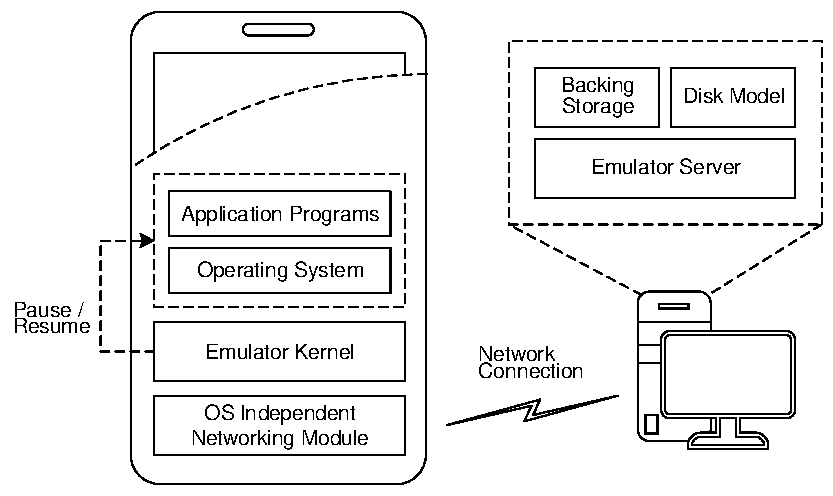
\includegraphics[width=0.9\textwidth]{figures/ch6-emulator-overview.pdf}
	\caption{\label{fig:ch6-emulator-overview}An overview of the proposed storage device emulator.}
\end{figure}

\begin{itemize}
	\item By pausing the state of the OS as necessary whenever the storage device is being emulated, the proposed storage device emulator can overcome the real-time timing constraints faced by emulators which are based on the conventional designs. This allows the proposed emulator to emulate storage devices that would be challenging or even impossible for the conventional storage device emulators. For example, the proposed emulator can allow disk models of arbitrary complexity to be used for simulating the behavior of the target storage device. Another problem with the conventional storage device emulation designs is that the backing storage must be faster than the storage device being emulated. In reality, faster storage devices tend to be more expensive and smaller in size. With the proposed storage device emulator, because the state of the OS is paused while the emulator is accessing the backing storage, slower storage devices can be used as the backing storage for emulating faster storage devices. For example, it is possible to use a slower conventional hard disk drive as the backing storage for emulating fast SSD devices that would otherwise be too large to fit into RAM.
	
	\item Unlike the complete machine simulation approach, there is no need to construct a complete machine simulation model for experimentation. Because the OS and the application programs are run directly on the native machine hardware, the detailed behaviors of the target machine hardware, such as the memory and cache hierarchies, the bandwidth and latencies of the system bus interconnects, and the micro-architecture of the CPU, can automatically be taken into account. Note that because the emulator kernel is also run on the target system's CPU, the cache state of the CPU might be affected. To minimize the disturbances that the proposed emulator might cause to the target system, the data buffers used by the proposed emulator can be allocated from non-cached memory regions. It is also worth noting that because of the way that the state of the OS is paused, the proposed storage device emulator also works with multiprocessor systems.
	
	\item The task of disk model simulation and actual data persistency is done by an emulator server running on a separate computer. This minimizes the interferences that the storage device emulator might cause to the target system. For example, the system memory of the target system does not need to be reserved for use as the backing storage. While it is possible to simulate the disk model directly on the target system while the OS is paused, simulating the disk model on a separate computer can reduce interfering with the cache localities of the target system.
	
	\item Network connection is used as the communication channel between the emulator kernel and the emulator server. Therefore, the features that can be supported by the emulated storage devices will not be limited by the actual I/O interface available on the target system. Furthermore, because the state of the OS is paused while the communications between the emulator kernel and emulator server are taking place, the reading and writing of the actual data for the emulated storage device can take as long as they are required to be transferred over the network channel. For example, for a read operation, the emulator kernel will complete the reading of the actual data of the I/O response from the emulator server before resuming the OS to the running state. This means that the bandwidth of the emulated storage device as perceived by the OS can exceed the bandwidth of the network channel being used. For example, it is possible to emulate storage devices that have transfer rates of over 100MB/s using a physical 802.11b wireless link, which only has a maximum transfer rate of 11Mbps. Moreover, the evaluation results will not be affected by the latencies and jitters of the network communication channel because all data transfers are carried out while the OS is in the paused state.
\end{itemize}

Table~\ref{tab:ch6-1} gives a summary of when and how the proposed storage device emulator could be advantageous compared to the other approaches.

\begin{table}[htbp]%
	\renewcommand{\arraystretch}{1.3}
	\centering
	\caption{Comparison of the proposed approach to the other approaches}\label{tab:ch6-1}
	\noindent\begin{tabularx}{\textwidth}{|p{2.8cm}|p{5.4cm}|X|}
		\hline
		\centering\bfseries Compared to & \centering\bfseries Possible Problems with the Other Approaches & \centering\bfseries\arraybackslash Advantages of the Proposed Approach \\ \hline
		
		\hyphenpenalty=10000\raggedright Complete machine simulation & The fidelity of the complete machine simulation model might not be a good approximation of the target system due to lack of exact models for critical SoC components. \newline\newline
		The speed of the complete machine simulation model might be too slow for conducting large full-system benchmarks. &
		By conducting the experiments using the real hardware of the target system, good system model fidelity and fast simulation speed can be achieved. \\ \hline
		
		\hyphenpenalty=10000\raggedright Conventional real-time storage device emulation &
		The time needed for simulating the disk model might be longer than the desired I/O response timings. \newline\newline
		The speed of the backing storage might be slower than the desired I/O response timings. &
		By pausing the state of the OS while the disk model is being simulated and the backing storage is being accessed, the proposed storage device emulator can spend as long as it requires on preparing the I/O responses. \\ \hline
		
		\hyphenpenalty=10000\raggedright Local virtual storage device emulation &
		The main memory available on the target system might be too small for emulating larger storage devices. &
		By offloading the emulation task to a separate remote server, the size of the emulated storage device can be as large as the backing storage available on the remote server. \\ \hline
		
		\hyphenpenalty=10000\raggedright Remote actual storage device emulation &
		The physical I/O interface available on the target system might not be fast enough (in terms of bandwidth and latency) for emulating the desired storage device. &
		By pausing the OS and transferring the actual data over the network links, storage devices of any speed can be simulated and made available to the OS. \\ \hline
		\end{tabularx}
\end{table}%

The design of the proposed storage device emulator is discussed in the following sections. In section~\ref{sec:ch6-6.1}, the concept of OS state pausing in the context of the proposed storage device emulator is explained. Section~\ref{sec:ch6-6.2} gives an overview of how OS state pausing is utilized in the proposed storage device emulator. Section~\ref{sec:ch6-6.3} describes the emulator server and explains the concept of disk model simulation time rollback, which is required for emulating storage devices that can support concurrent I/O request processing and I/O request prioritization. The detailed operation of the proposed storage device emulator is presented in section~\ref{sec:ch6-6.4}, and finally, the OS independent network subsystem is discussed in section~\ref{sec:ch6-6.5}.

\section{Operating System State Pausing}
\label{sec:ch6-6.1}

The state of the OS can be viewed as composed of the combined state of all the processes running in the OS and the current values in the clock counter and the hardware timers used by the OS. By freezing the execution of all the processes in the OS and stopping the clock counter and the hardware timers, the state of the OS can be paused. In the proposed storage device emulator, the state of the OS is paused by the emulator kernel using the following procedure:
\begin{enumerate*}[label=(\roman*)]
	\item Stop the clock counter and the hardware timers by programming their control registers.
	\item If the target platform is a symmetric multiprocessor system, use IPIs (inter-processor interrupts) to interrupt all the other CPUs in the system and schedules a high priority busy waiting loop on them. The busy waiting loop will prevent the other CPUs from executing any processes that belongs to the OS.
\end{enumerate*}

The execution of the OS is resumed from the paused state using the following procedure: 
\begin{enumerate*}[label=(\roman*)]
	\item Resume the counting of the clock counter and the hardware timers.
	\item Terminate the busy waiting loops so that all the CPUs will resume to their original work.
\end{enumerate*}
The pausing and resuming of the OS is entirely transparent to the applications running on the OS, and the OS can still correctly service any system calls requested by the applications. Therefore, all user space applications can be run unmodified on the proposed system.

While the OS is in the paused state, the emulator kernel will not be able to utilize certain OS services such as interrupts or timers. Therefore, a polling-based OS independent networking module which does not rely on interrupts or system timers is design for use by the emulator kernel to communicate with the emulator server. The details of the OS independent networking module will be further discussed in section~\ref{sec:ch6-6.5}.

Because of the pausing made to the OS, the system time that the OS observes is no longer linked to the real-world time. Instead, a virtual system time which is derived from the value in the clock counter is observed by the OS. To preserve the original system behavior, all the external events to the OS should be scheduled according to the virtual system time. In the proposed storage device emulator, the only external events that need to be considered are the completion signals from the emulated storage device and the timer interrupts. The design of the proposed storage device emulator makes sure that the response signals from the emulated storage device are delivered to the OS according to the virtual system time.

In the ideal case, the state of the OS right before being paused and right after being resumed should be exactly the same. However, there are three factors which can affect the deviation of the OS states before and after pausing:

\begin{itemize}
	\item The first factor is the resolutions of the clock counter and the hardware timers. Each time that the counting of the clock counter and the hardware timers are paused and then resumed, the fraction values that are currently accumulated in the digital circuits will be lost. For example, if the clock counter has a resolution of 1\si{\micro\second}, then any passage of time that is less than 1\si{\micro\second} will be lost when the clock counter is paused by writing to its control registers. In our experimental environment, the resolutions of the clock counter and the hardware timers used by the Linux OS is approximately 3\si{\nano\second}.
	
	\item The second factor is how fast the other CPUs in the system can be put into the busy waiting loop. In the ideal case, the other CPUs in the system should be switched immediately to execute the busy waiting loop as soon as the clock counter and the hardware timers are paused. However, it is possible that the other CPUs in the system will have their interrupts disabled when the IPIs are issued. In this case, the busy waiting loop will have to wait until the interrupts are enabled again. During this period of time, the other CPUs would have completed additional tasks that are not supposed to be done when the OS is in the paused state. On systems that can support non-maskable IPIs, such as the NMI in the x86 processors~\cite{Intel:2013} or the FIQ in the ARM processors, the non-maskable IPIs can be used to immediately put the other CPUs into the busy waiting loop regardless of their interrupt enabling states. In practice, the CPUs in a properly designed system should not be in the interrupt-disabled state for any long periods of time.
	
	\item The third factor is the effect of the CPU cache disturbance. When the OS is in the paused state, the CPU of the target system will need to execute instructions for handling the communication between the emulator kernel and the emulator server, and therefore the cache state of the CPU will be different before and after OS pausing. To get an ideal of the scale of the disturbance that the proposed emulator will have on the target system's CPU cache states, we used the \textit{ftrace}~\cite{Kernel:2014} function tracer in the Linux kernel to trace the kernel execution path for handling I/O requests. With the proposed emulator emulating a virtual storage device, the sizes of instruction codes executed by the CPU for handling a read or write request from user space is approximately 101KB and 151KB, respectively. Compared to a simple local storage device emulation type emulator, the sizes of instruction codes executed by the CPU for handling a read or write request is approximately 91KB and 140KB, respectively. Since the L2 cache size of the CPU used in our experimental platform is 512KB, the additional cache overhead introduced by the proposed emulator is only less than 2\% of the L2 cache. Furthermore, modern embedded processors are likely to have larger caches. For example, the Apple A7 SoC~\cite{wiki:2015:A7} incorporates a 1MB L2 cache and a 4MB L3 cache. The cache disturbance that the proposed emulator will have on those processors would be even less.
\end{itemize}

Even though there could be some slight deviations of the OS states before and after pausing, if the scale of the deviations is small compared to the frequency of its occurrence, then the overall system behavior would still be close enough to the original target system for conducting performance studies. In the proposed emulator, the frequency that the OS state pausing is happening is roughly proportional to the frequency that the I/O requests are processed by the emulated storage device. The scale of the deviation of our experimental platform is at the nanoseconds level, and from the experimental results, we have validated that the proposed OS state pausing approach is effective for emulating storage devices that have service times at the millisecond and microsecond levels.

\section{Operating System State Pausing and Storage Device Emulation}
\label{sec:ch6-6.2}

This section discusses how OS state pausing is utilized in the proposed storage device emulator. During operation, the OS in the proposed storage device emulator is either in the paused state or in the running state. To avoid having a real-time timing constraint on the progressing speed of the emulator server and the performance of the communication channel between the emulator kernel and the emulator server, the emulator kernel is designed to only make requests to the emulator server when the OS is in the paused state. The OS will be put into the paused state whenever the emulator kernel is waiting for the responses from the emulator server for the information that it needs for emulating the storage device. That is, the OS and the emulator server will never be in the operating state at the same time. In other words, the synchronization between the emulator kernel and the emulator server only happens when the OS is in the paused state.

Before resuming the OS back to the running state, the emulator kernel will need to have all the information that it needs for emulating the storage device until the next time point that it will communicate with the emulator server. To achieve this, the emulator server is designed to simulate the disk model to a future time point at which the information of the next I/O response can be determined while the OS is in the paused state.

When the OS is put back to the running state, the emulator kernel will use the information provided by the emulator server to set a timer interrupt at the completion time of the next I/O response. Because the timer service provided by the OS is utilized, the completion times of the I/O responses will automatically be scheduled according to the virtual system time of the OS. When the emulator kernel is notified by the timer interrupt, the corresponding I/O response will then be replied to the OS at the desired completion time as indicated by the disk model.

\begin{figure}[htpb]
	\centering
	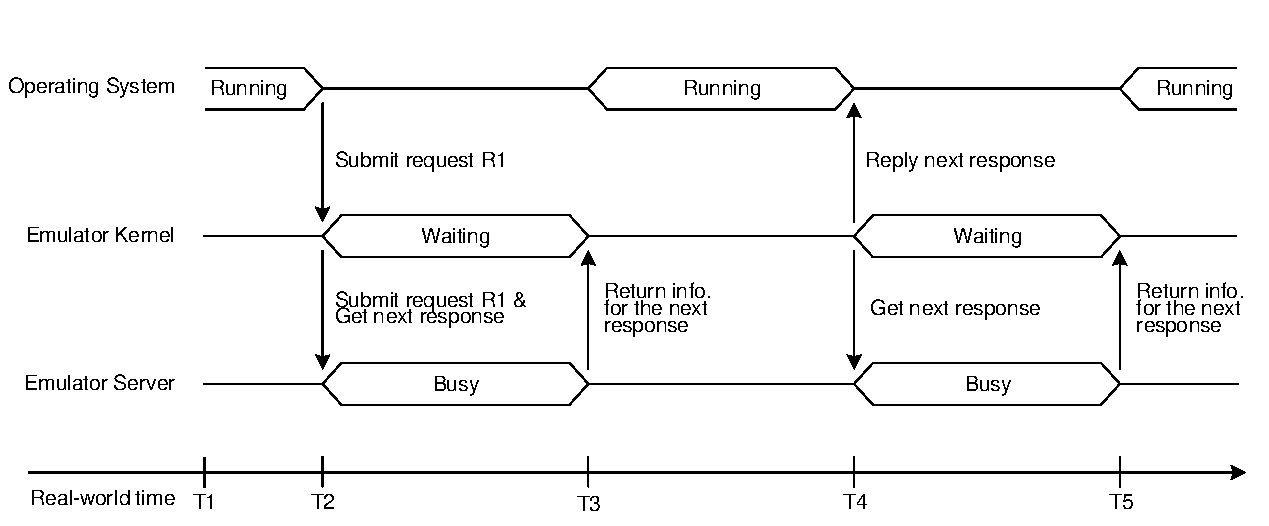
\includegraphics[width=\textwidth]{figures/ch6-fig-6.pdf}
	\caption{\label{fig:ch6-fig-6}Interactions between the OS, the emulator kernel, and the emulator server.}
\end{figure}

A sequence diagram is illustrated in Figure~\ref{fig:ch6-fig-6} to show an example interaction between the OS, the emulator kernel, and the emulator server. As previously shown in Figure~\ref{fig:ch6-emulator-overview}, the emulator kernel is run on the same machine as the OS and the emulator server is run on a separate computer.

At T1, the OS is running continuously and the emulator server is in the idle mode waiting for commands from the emulator kernel. AT T2, an I/O request, R1, is generated by the OS. As soon as R1 is received, the emulator kernel will pause the state of the OS and submit the parameters about R1 to the emulator server. The actual data of R1 is also submitted to or retrieved from the emulator server depending on whether R1 is a read or a write request.

After submitting the I/O request R1, the information for the next I/O response is requested by the emulator kernel. The information of an I/O response includes the ID and the completion time of the I/O response. Because the OS is paused while the emulator server is processing the commands from the emulator kernel, the time between T2 and T3 can be arbitrary long. Before resuming the execution of the OS at T3, the emulator kernel will set a timer event to interrupt itself at the corresponding completion time of the next I/O response. When woken up by the timer interrupt, the emulator kernel can then reply the next I/O response to the OS.

Notice that the emulator kernel asks for the information for the ``next'' I/O response and not specifically for the information for R1, which is the most recently submitted I/O request. This is because that the next I/O request that will be completed by the emulated storage device might not be R1. For example, if the emulated storage device supports I/O prioritization and that it is currently servicing an I/O request that has a higher priority than R1, then R1 will not be serviced until the previous I/O request has been completed. Another example is that if the emulated storage device supports processing of concurrent I/O requests and that there is an I/O request, for example R0, which is currently being processed, then it is possible that R0 will be completed before R1.

Please note that as far as the emulator kernel is concerned, it does not need to know the reason of why the ``next'' I/O response is different from the most recently submitted I/O request. The important thing is that the interface between the emulator kernel and the emulator server will permit the emulator server to change the answer for the next I/O response due to I/O requests that are later submitted to the emulator server.

After the I/O response is replied to the OS at T4, the emulator kernel will communicate with the emulator server again to determine if there will be another I/O response that is going to be completed by the emulated storage device. If there is, then the emulator kernel will set a timer event to interrupt itself at the corresponding completion time of that next I/O response. On the other hand, if there is no further I/O response from the emulated storage device, then the emulator kernel will leave the OS in the running state until future I/O requests are generated by the OS.

\section{Emulator Server with Disk Model Simulation Time Rollback Support}
\label{sec:ch6-6.3}

The emulator server is responsible for simulating the disk model and persisting the actual data for the emulated storage device. It is designed to handle four types of commands from the emulator kernel, which are described in Table II.

\begin{table}[htbp]%
	\renewcommand{\arraystretch}{1.3}
	\centering
	\caption{Commands supported by the emulator server}\label{tab:ch6-2}
	\noindent\begin{tabulary}{\dimexpr\textwidth-3.5cm}{|p{3.5cm}|L|J|}
		\hline
		\centering\bfseries Command Type & \centering\bfseries Parameters & \centering\bfseries\arraybackslash Description \\ \hline
		
		\textit{Reset} &
		\textit{Disk size},\vspace{0.5em}\newline
		\textit{Backing storage configuration},\vspace{0.5em}\newline
		\textit{Disk model configuration} &
		The \textit{reset} command initializes the state of the emulator server to prepare for emulating a new storage device. The \textit{disk size} parameter specifies the size of the storage device to be emulated. The \textit{backing storage configuration} is used for selecting the backing storage device to use (for example, RAM or SSD). The characteristics of the target storage device to be emulated can be controlled by the disk model configuration. For example, the disk model in our experimental implementation can support the configuration of \textit{speedup factor} and the \textit{number of channels}. \\ \hline
		
		\textit{Data Transfer} &
		\textit{Sector number},\vspace{0.5em}\newline
		\textit{Read/write type},\vspace{0.5em}\newline
		\textit{Sector data} &
		The \textit{data transfer} commands are used for the persistence of the actual data. The write data transfer command is used to save the actual data to the backing storage, and the read data transfer command is used for retrieving the actual data from the backing storage. \\ \hline
		
		\textit{Submit Request} &
		\textit{Request time},\vspace{0.5em}\newline
		\textit{Start sector},\vspace{0.5em}\newline
		\textit{Sector count},\vspace{0.5em}\newline
		\textit{Read/write type} &
		The \textit{submit request} command is used for submitting I/O requests to the emulator server. The emulator server will keep track of the I/O requests that have been received and it will simulate the disk model accordingly.\\ \hline
		
		\textit{Get Next Response} &
		\textit{OS system time} &
		The emulator kernel uses the \textit{get next response} command to get the information for the next I/O response that will be completed by the emulated storage device. If there are no I/O requests being processed by the emulated storage device, then the return value of this command will indicate that there will be no next response. \\ \hline
	\end{tabulary}
\end{table}%


In order to support the \textit{get next response} command, the emulator server will need to simulate the disk model past the current system time of the OS. When simulating the disk model between the current system time of the OS and until the completion time of the next I/O response, the disk model is simulated under the assumption that the OS will not submit any additional I/O requests to the emulated storage during this period of time. For example, if an I/O request is submitted to the emulator server at V1 and the next I/O response is determined to be completed at V3, then the disk model is simulated under the assumption that the OS will not submit any I/O request to the emulated storage device between V1 and V3. This assumption is required because the disk model is being simulated into the ``future'' time. However, this assumption might not always be true if the emulated storage device can handle more than one I/O requests from the OS. For example, if another I/O request is generated by the OS between V1 and V3, then the state of the disk model will need to be \textit{rolled back} to a prior simulation time at which when the new I/O request is generated. The disk model can then be simulated again with the new I/O request being taken into account.

\begin{figure}[htpb]
	\centering
	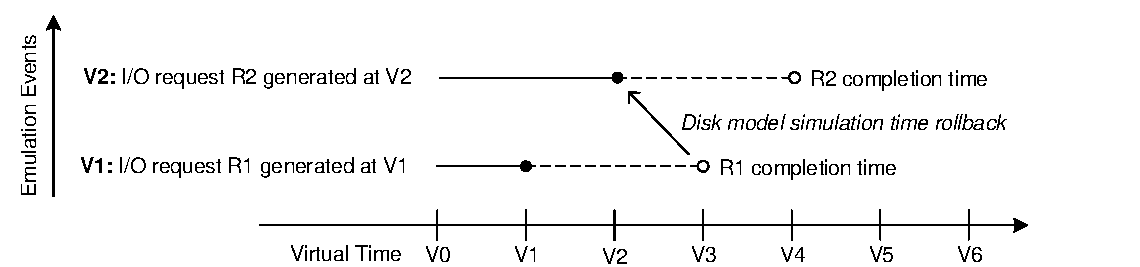
\includegraphics[width=\textwidth]{figures/ch6-fig-7.pdf}
	\caption[Disk model simulation time rollback.]{\label{fig:ch6-fig-7}A scenario showing the emulator server performs a disk model simulation time rollback. Solid circles represent the virtual system time of the OS and white circles represent the simulation time of the disk model.}
\end{figure}

An example is illustrated in Figure~\ref{fig:ch6-fig-7} to show a scenario when disk model simulation time rollback is performed by the emulator server. At virtual time V1, an I/O request, R1 is generated by the OS. Assume that R1 is the only I/O request currently submitted to the emulated storage device and that R1 will be completed by V3 if the emulated storage device does not receive any other I/O requests before V3. When the \textit{get next response} command is issued to the emulator server at V1, the disk model will be simulated to until time V3, at which it is the time that R1 will be completed. The emulator kernel will use the replied information to set a timer to be expired at V3 so that R1 will be replied to the OS when the system time of the OS reaches V3. After setting the timer, the emulator kernel will put the OS back into the running state. Now, assume that the OS has generated another I/O request, R2, when the system time reaches V2. The emulator kernel will then submit R2 to the emulator server and issue another \textit{get next response} command. At this time, the simulation time of the disk model will need to be rolled back to V2 so that I/O request R2 can be properly considered by the disk model.

For example, if R2 has a higher priority than R1, then after the disk model is rolled back to V2, the disk model will determine that the processing of R1 should be preempted by R2. Therefore, when the emulator kernel issues a \textit{get next request} command at V2, the emulator server will reply that the next I/O response is R2. For another example, if the emulated storage device supports concurrent I/O request processing and that R2 has a shorter service time than R1, then even that R2 is received after R1, its completion time might still be earlier than V3. In this case, even if the processing of R1 is not interrupted by R2, the next I/O request that will be completed by the emulated storage device will still change to R2.

In the actual implementation of the emulator server and the disk model, the simulation time of the disk model might not be able to be rolled back to any arbitrary point of time. To allow the rollback of the disk model to any arbitrary point of time would require that every state progression of the disk model to be saved, which might not be practical. A design technique can be used so that the state of the disk model is only saved at the time point at which the \textit{get next response} command is received. With this design technique, the simulation time of the disk model is first rolled back to the previous state at which the previous \textit{get next response} command is issued, and the disk model can then be simulated from there on. Using the scenario illustrated in Figure~\ref{fig:ch6-fig-7} as an example: when the \textit{get next response} command is received at V2, the disk model is rolled back from V3 to V1 and then simulated starting from V1. Between V1 and V2, the disk model will only consider R1. And from V2 and on, the disk model will consider both R1 and R2. With this design technique, supporting disk model simulation time rollback would only require that the emulator server to be able to roll back the disk model to the states at which the previous \textit{get next response} commands are received. This can greatly simplify the design and implementation of the emulator server and the disk model.

For each rollback operation, the amount of work that is discarded is approximately equal to the amount of time for simulating one I/O request. For example, if on average it takes the disk model T units of time to simulate an I/O request, then the cost of each rollback operation, which equals to the discarded simulation progress of the disk model, will be approximately T units of time.

The upper bound for the frequency at which the rollback operations will be occurring during simulation is no more than the number of I/O requests being submitted to the emulator server. For each I/O request submitted to the emulator server, at most one rollback operation could be triggered. That is, if the submission time of the I/O request is earlier than the earliest completion time of the I/O requests already in the disk model, then one rollback operation will be performed on the disk model. Therefore, for N I/O requests, the maximum number of rollback operations that could have occurred will not exceed N.
\section{Detailed Operation of the Proposed Storage Device Emulator}
\label{sec:ch6-6.4}

\begin{figure}[htpb]
	\centering
	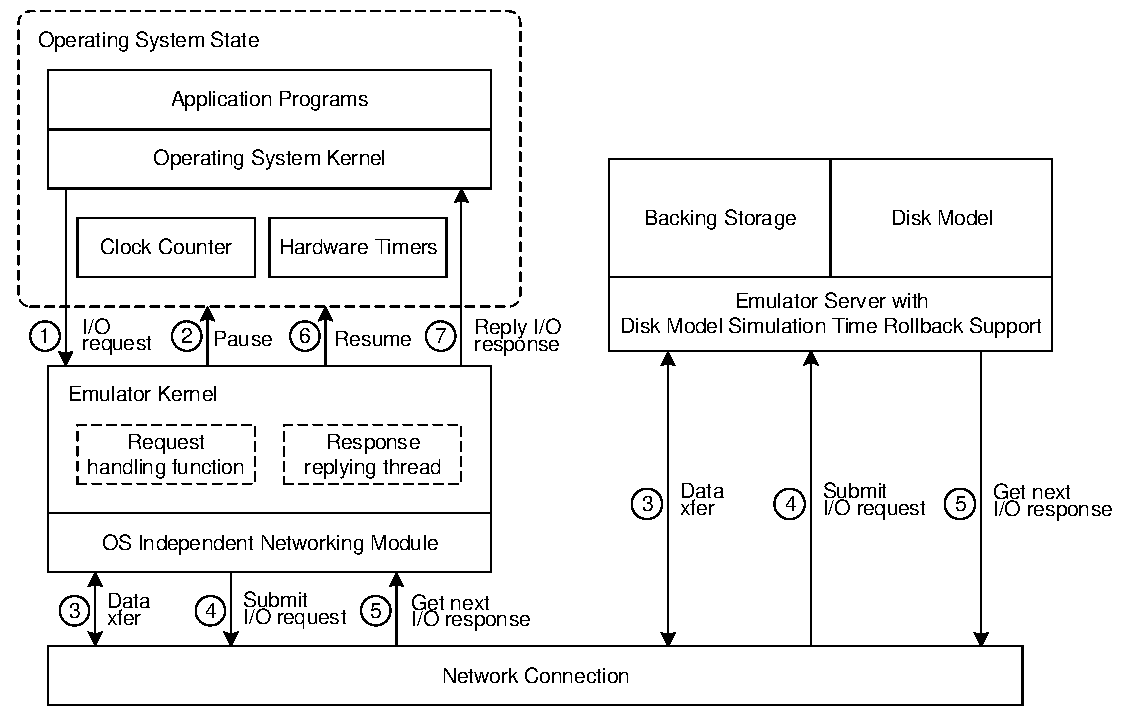
\includegraphics[width=\textwidth]{figures/ch6-fig-8.pdf}
	\caption{\label{fig:ch6-fig-8}Detailed operation of the proposed storage device emulator.}
\end{figure}

A more detailed view of the proposed storage device emulator is illustrated in Figure~\ref{fig:ch6-fig-8}. The emulator kernel is responsible for emulating a virtual storage device to the OS at the block device driver level and is composed of two primary components: the request handling function, (described in algorithm listing~\ref{alg:request-handling-function}) and the response replying thread (described in algorithm listing~\ref{alg:response-replying-thread}). The request handling function is part of the block device driver that is registered to the OS. Whenever the OS generates I/O requests towards the emulated storage device, it will invoke the request processing function.

The response replying thread is a high priority background kernel thread used for replying the I/O responses to the OS. When the completion time of an I/O response is determined, the emulator kernel will set a timer event which will wake up the response replying thread at the corresponding completion time. When the response replying thread is woken up, it will then reply the I/O response to the OS.

The detailed operation steps of the proposed storage device emulator depicted in Figure~\ref{fig:ch6-fig-8} are discussed as follows.

\begin{description}
	\item[Step 1:] Receive I/O request from the OS. When an I/O request is generated by the OS, the request handling function in the emulator kernel will be invoked. A set of non-cacheable memory buffers in the emulator kernel are used to simulate the memory mapped I/O interface of the storage device controller. If the I/O request from the OS is a write request, then the actual data will be copied to the write buffer (the \textit{tempWriteBuffer} in the algorithm listings) of the emulator kernel at this time to mimic the transferring of the actual data to the storage device controller.
	
	\item[Step 2:] Pause the state of the OS. The state of the OS will be paused by the emulator kernel before initiating communication to the emulator server. This allows the emulator server to take as long as it requires for processing the commands from the emulator kernel without affecting the behavior of the emulated storage device as perceived by the OS.
	
	\item[Step 3:] Transfer the actual data of the I/O request. If the I/O request is a write request, then the data that was copied to the write buffer (\textit{tempWriteBuffer}) in step 1 will be transferred to the emulator server for persistence. Otherwise, if the I/O request is a read request, then the actual data of the I/O request will be retrieved from the emulator server and stored in the non-cacheable read buffer (the \textit{tempReadBuffer} in the algorithm listings) of the emulator kernel. The retrieved actual data is not copied directly to the I/O response buffers that belong to the OS at this time to mimic the behavior of real storage devices. For real storage devices, the requested actual data will not be available until the I/O request is completed. If the actual data is copied to the I/O response buffers that belong to the OS at this time, then the temporal cache locality of the actual data will be different from that of the real-world cases. The retrieved actual data will temporarily wait in the read buffer until the I/O response is actually going to be replied to the OS in step 7. At that time, the actual data will then be copied from the read buffer to the I/O response buffers that belong to the OS.
	
	\item[Step 4:] Submit the I/O request to the emulator server. The parameters of the I/O request, which includes the request time, request type (read or write), start sector, and number of sectors, is submitted to the emulator server. These information are used by the disk model to simulate the completion time of the I/O requests.
	
	\item[Step 5:] Get the information of the next I/O response. Before resuming the OS from the paused state, the emulator kernel needs to know the completion time of the next I/O response. A timer event will be set to wake up the response replying thread at the corresponding completion time. If there is a timer event already set for the response replying thread, then the timer event will be updated to the new completion time if it is earlier than the current value set in the timer.
	
	\item[Step 6:] Resume the OS from the paused state. After the response replying thread is properly set to be woken up at the completion time of the next I/O response, the OS will be resumed from the paused state. The OS then runs continuously until one of the two following scenarios happens:
\begin{enumerate*}[label=(\roman*)]
	\item Another I/O request is generated by the OS. In this case, the newly generated I/O request is handled following the same steps beginning from step 1.
	\item The timer event for the response reply thread expires and the response replying thread is woken up. In this case, the processing continues to step 7.
\end{enumerate*}	

	\item[Step 7:] Reply the I/O response to the OS. When the system time of the OS has advanced to the completion time of the next I/O response, the response replying thread will be woken up by the timer event. If the I/O response is for a write request, then the response relying thread simply notifies the OS that the write request has been completed. Otherwise, if the I/O response is for a read request, then the actual data in the \textit{tempReadBuffer} will be first copied to the corresponding I/O response buffers that belong to the OS, and then the OS will be notified about the completion of the read request.
\end{description}


\begin{algorithm}
\small
\newcommand*\Let[2]{\State #1 $\gets$ #2}
	\caption{Request Handling Function
		\label{alg:request-handling-function}}
	\begin{algorithmic}[1]
		\Function{request_fn}{}
		\Let{Request}{get next pending request from OS}
		\If{Request is a write request}
			\Let{Request.tempWriteBuffer}{Sector data}
		\EndIf
		\State Pause OS
		\If{Request is a write request}
			\State Transfer Request.tempWriteBuffer to emulator server;
		\Else
			\Let{Request.tempReadBuffer}{Retrieve sector data from emulator server}
		\EndIf
		\Let{HasNextResponse_T, NextResponseTime_T, NextResponses_T}{Emulator server}
		\If{HasNextResponse_T == TRUE and \newline (HasNextResponse == FALSE or NextResponseTime_T < NextResponseTime)} \label{lst1:line:if}
			\Let{HasNextResponse}{TRUE}
			\Let{NextResponseTime}{NextResponseTime_T}\label{lst1:line:assignNextResponseTime}
			\Let{NextResponses}{NextResponses_T}
			\State{Signal the response replying thread}\label{lst1:line:signal}
		\EndIf
		\State Resume OS

		\EndFunction
	\end{algorithmic}
\end{algorithm}

Remarks on algorithm~\ref{alg:request-handling-function}: In Linux, the request handling function is invoked by the kernel whenever there are I/O requests to be submitted to the storage device. Request.tempWriteBuffer is a non-cached memory buffer for temporarily storing the sector data of a write I/O request. Request.tempReadBuffer is a non-cached memory buffer for temporarily storing the sector data of a read I/O request. The temporary buffers are allocated from a non-cached memory address space to simulate what a real device driver would do. That is, the sector data need to be transferred between the CPU and the device controller. The HasNextResponseTemp, NextResponseTimeTemp, and NextResponsesTemp variables store the information regarding the next I/O response from the emulator server. The if clause in line~\ref{lst1:line:if} tests if the completion time of the new next I/O response will be earlier than the current timer interrupt of the response replying thread. If true, then the response replying thread will be signaled so that the timer interrupt can be updated to an earlier time point corresponding to NextResponseTimeTemp. Note that the request handling function only makes requests to the emulator server while the OS is being put into the paused state.

\begin{algorithm}
	\small
	\newcommand*\Let[2]{\State #1 $\gets$ #2}
	\caption{Response Replying Thread
		\label{alg:response-replying-thread}}
	\begin{algorithmic}[1]
		\State{HasNextResponse = FALSE}
		\Repeat
		\If{HasNextResponse == FALSE} \label{lst2:line:startSleep}
			\State{Sleep until being signaled}
		\EndIf \label{lst2:line:endSleep}
		\Repeat \label{lst2:line:startWaitTimeArrive}
			\State{Sleep until NextResponseTime has arrived or being signaled}
		\Until{NextResponseTime has arrived} \label{lst2:line:endWaitTimeArrive}
		\For{each Response in NextResponses} \label{lst2:line:startReply}
			\If{Response is a read response}
				\State Copy Response.tempReadBuffer to the response buffers belonging to the OS
			\EndIf
			\State Reply Response to operating system
		\EndFor \label{lst2:line:endReply}
		\State Pause OS
		\Let{HasNextResponse, NextResponseTime, NextResponses}{Emulator server} \label{lst2:line:getInfo}
		\State Resume OS
		\Until{Storage emulator is stopped}
	\end{algorithmic}
	\bigskip
\end{algorithm}

Remarks on algorithm~\ref{alg:response-replying-thread}: The response replying thread is a high priority background kernel thread responsible for replying the I/O responses to the OS. In line~\ref{lst2:line:startSleep} to~\ref{lst2:line:endSleep}, if there is currently no I/O response pending to be replied to the OS, the response replying thread will go into an infinite sleep until being signaled by line~\ref{lst1:line:signal} of the request handling function. The while loop between line~\ref{lst2:line:startWaitTimeArrive} and~\ref{lst2:line:endWaitTimeArrive} ensures that the timer interrupt which will wake up the response replying thread is set to the most current value assigned by the request handling function (line~\ref{lst1:line:assignNextResponseTime} of the request handling function). Line~\ref{lst2:line:startReply} to~\ref{lst2:line:endReply} replies the I/O response to the OS when the completion time of the I/O request has arrived. After the I/O response has been replied to the OS, line~\ref{lst2:line:getInfo} gets the information for the next I/O response from the emulator server. Note that the response replying thread only makes requests to the emulator server while the OS is put into the paused state.

\section{Operating System Independent Networking Module}
\label{sec:ch6-6.5}

An OS independent networking module is designed in the proposed storage device emulator to be used by the emulator kernel for communicating with the emulator server. The OS independent networking module is used instead of the standard networking stack that comes with the OS because of the following reasons:

\begin{itemize}
	\item While the OS is in the paused state, the CPUs will have their interrupts disabled. The network device drivers that come with the OS cannot be used because they depend on interrupts for working with the network hardware. In the OS independent networking module, a special polling-based network device driver is implemented for working with the network hardware. The special device driver provides its own set of polling-based APIs for use by the emulator kernel.
	
	\item To minimize the interference that the OS independent networking module will have to the original system behavior, the packet buffers which are used by the network hardware are not allocated from the OS kernel. Instead, a packet buffer manager is designed for allocating and reclaiming the packet buffers from a non-cached memory pool owned by the emulator kernel.
	
	\item When the OS is in the paused state, the timer service provided by the OS will not function properly because the clock counter and the hardware timers are stopped. This means that the TCP implementation in the standard OS networking stack will not work because the retransmission timers will not be functioning correctly. In the proposed storage device emulator, the emulator kernel communicates with the emulator server using the UDP protocol. The UDP packets are assembled and parsed by the emulator kernel without going through the full OS networking stack. To transmit a UDP packet, the UDP packet is assembled by the emulator kernel and handed to the special polling-based device driver in the OS independent networking module directly. To receive the response packet, the emulator kernel uses the polling-based API to poll the network hardware repeatedly until the expected packet has arrived. If the expected response packet is not received after a certain number of polling attempts, the request packet will be retransmitted again by the emulator kernel.
\end{itemize}

\section{Experimental Results}
\label{sec:ch6-6.6}

We have implemented the proposed storage device emulator with the Linux OS. The target hardware platform used is the ZedBoard development board~\cite{ZedBoard:2014}. ZedBoard contains a 667MHz dual-core ARM Cortex-A9 MPCore processor and 512MB of DDR3 main memory. The Linux kernel used is based on the kernel version 3.10.0 from the Xilinx source repository~\cite{Xilinx:2014:kernel}. The root file system used is based on the nano build of the Linaro release version 13.11~\cite{Linaro:2014:v13.11nano}. The device driver for the ARM global timer~\cite{Xilinx:2013:Zynq7010} is backported from the mainline kernel~\cite{Kernel:2013:ARMglobalTimer}, and the Linux kernel is configured to use the ARM global counter as its clocksource and clockevent devices~\cite{Stultz:2005} \cite{GleixnerNiehaus:2006} \cite{GleixnerMolnar:2006} \cite{Gleixner:2007}. The ARM global timer runs at half the speed of the ARM processor. At 333MHz, it provides the clocksource and clockevent devices a timing resolution of approximately 3\si{\nano\second}. In other words, the resolution of the clock counter and hardware timers used by the Linux OS is approximately 3\si{\nano\second}. The emulator server is implemented as a user space program on a separate computer running Ubuntu Linux. The host computer for the emulator server is equipped with an Intel Core i5-3210M CPU running at 2.5GHz, 4GB of RAM, and a Seagate Momentus Thin 320GB hard disk drive as the backing storage. ZedBoard is connected to the emulator server using a 1Gbps Ethernet LAN. 

To measure how much disturbance the operations of the proposed emulator (e.g., OS pausing, OS resuming, network communication, etc.) will have to the target system, the simulation results from the proposed emulator are compared to the results from a reference system.

The reference system is an unmodified Linux OS, which runs on the same ZedBoard platform, and has a RAMDISK storage device emulated by a local emulation type emulator. The parameters of the RAMDISK device are designed so that its performances are comparable to UHS-1 SD cards. The same disk model will be used by both the proposed emulator and the reference system. Ideally, the disturbances caused by the operations of the proposed emulator should be low and the evaluation results from the proposed emulator should match closely to the results from the reference system.

The reasons of why a RAMDISK device, which is emulated by a local emulation type emulator, instead of real storage devices is used in the reference system are given as follows:

\begin{itemize}
	\item The structure of the emulator kernel is very similar to how a local emulation type emulator would be implemented. The main differences between the proposed emulator and a local emulation type emulator are the extra steps needed for pausing and resuming the OS and for performing network communications. Using a local emulation type emulator in the reference system allows us to measure how much disturbance the extra operations of the proposed emulator has caused to the target system.
	
	\item In our experience, the work needed for accurate modeling of real storage devices is not trivial. For example, to model the exact behavior of a NAND storage device that contains a Flash Translation Layer (FTL) would require that the firmware of the FTL to be available; otherwise, the exact sector data placement in the emulated storage device will be different from the real device, and this will lead to different I/O response timings. If the behaviors of the real storage device are not modeled exactly, then testing the proposed emulator using an inexact disk model will mean that we will not be able to tell if the inaccuracies are caused by the disturbances of the proposed emulator or the inaccuracy of the disk model.
	
	\item The physical I/O interface on the target platform might limit the performances or characteristics of the real storage devices that can be tested. For example, the SD interface supported by the ZedBoard is at version 2.00, which can only support a maximum bus speed of 25MB/s. Therefore, it is not possible to validate the proposed emulator with a real SD device faster than 25MB/s on the ZedBoard platform. With a local emulation type emulator, we were able to emulate storage devices that have speeds of over 100MB/s for validating the proposed storage device emulator, which will not be possible if real storage devices are used. Moreover, next generation standards, such as the JEDEC Universal Flash Storage (UFS), will support the command queuing feature, and therefore cannot be emulated over the SD interface. By comparing against a local emulation type emulator, we were able to validate the proposed emulator under concurrent I/O scenarios.
	
	\item Besides using different I/O workloads for testing the proposed storage device emulator, we also want to test if the proposed emulator can handle storage devices of different speeds and concurrency levels. By using a local emulation type emulator as the comparison target, storage devices of different speeds and concurrency levels can easily be modeled for testing.
\end{itemize}
 
\begin{table}[htbp]%
	\centering
	\caption{Performance numbers used for the baseline storage device}\label{tab:ch6-3}
	\noindent\begin{tabular}{lcccc}
		\toprule
		& \multicolumn{2}{c}{Random Workload} & \multicolumn{2}{c}{Sequential Workload} \\
		\cmidrule(lr){2-3}
		\cmidrule(lr){4-5}
		\parbox{3cm}{\centering Transfer size} & \parbox{2cm}{\centering Read (\si{\milli\second}) } & \parbox{2cm}{\centering Write (\si{\milli\second}) } & \parbox{2cm}{\centering Read (\si{\milli\second}) } & \parbox{3cm}{\centering Write (\si{\milli\second})} \\
		
		\midrule
		
		512 bytes & 0.0051 & 1.1136 & 0.0019 & 0.0092 \\
		1 KB & 0.0053 & 1.1123 & 0.0020 & 0.0095 \\
		2 KB & 0.0054 & 1.1136 & 0.0023 & 0.0099 \\
		4 KB & 0.0057 & 1.1601 & 0.0027 & 0.0115 \\
		8 KB & 0.0063 & 1.2853 & 0.0033 & 0.0136 \\
		16 KB & 0.0071 & 1.2579 & 0.0036 & 0.0035 \\
		32 KB & 0.0096 & 2.2222 & 0.0068 & 0.0070 \\
		64 KB & 0.0151 & 2.7027 & 0.0139 & 0.0137 \\
		
		\bottomrule
	\end{tabular}
\end{table}%

The random and sequential read/write performances of a Transcend Ultra High Speed (UHS) Speed Class 1 SD memory card are measured and used to model a hypothetical baseline storage device. The measured performance numbers are shown in Table III. It is important to note that the baseline storage device is by no means trying to simulate the actual behavior of the Transcend SD memory card. These performance numbers are used for modeling the baseline storage device so that the performance of the baseline storage device is in line with the current top of the line storage devices.

The characteristics of the baseline storage device can be controlled by two parameters: the speedup factor and the number of channels parameters. Both parameters are varied from $\times$1 to $\times$4 for deriving a total of 16 storage device configurations for validating the proposed storage device emulator. The storage device configuration ChN-xS means that the number of channels the storage device has is N and it has a speedup factor of S. The number of channels parameter configures the number of concurrent I/O requests that the storage device can process simultaneously. For example, if four I/O requests are submitted to an emulated storage device which has four channels, then all four I/O requests will be processed concurrently. The speedup factor parameter configures how much faster the storage device is compared to the baseline storage device. For example, a speedup factor of two means that the response times of the emulated storage device will be half of the baseline storage device.

The total amount of memory available on ZedBoard is only 512MB. Therefore, the size of the emulated storage device is set to be 400MB, which leaves 112MB of memory for use by the Linux OS. A 12MB tmpfs temporary file storage is created and used for temporarily storing the outputs from the benchmark applications. Note that for the proposed storage emulator, because the actual data is persisted on the remote host, the Linux OS will be able to use the complete 512MB of main memory. However, we still configure the Linux OS to use only 112MB of memory so that the testing conditions are equivalent to the reference system.

The benchmarks are executed using the auto-pilot automation framework~\cite{Wright:2005:auto-pilot} \cite{Wright:2007:auto-pilot}. Each benchmark is run at least 10 times and until the radius of the 95\% confident interval is less than 5\% of the mean. The \textit{cron} and \textit{rsyslog} services in the Linux OS are disabled while the benchmarks are performed to reduce possible interferences. The system is rebooted after each benchmark run. The evaluation results are presented in the following subsections.
	
\subsection{Sequential Read Bandwidth}
\label{sec:ch6-6.6.1}

\begin{table}[htbp]%
	\small
	\begin{center}
	\caption{Sequential read bandwidth}\label{tab:ch6-5}
	\hspace*{-2cm}
	\noindent\begin{tabular}{
			l
			S[table-format=3.2]
			S[table-format=3.2]
			S[table-format=3.2]
			S[table-format=3.2]
			S[table-format=3.2]
			S[table-format=3.2]
			S[table-format=1.2]
			S[table-format=1.2]
			c}
		\toprule
		{Test Config} & {Mean} & {Median} & {Low} & {High} & {Min} & {Max} & {SDEV\%} & {HW\%} & \multicolumn{1}{c}{Diff} \\
		\midrule
		
		Ch1-x1 Ref. & 36.58 & 36.58 & 36.52 & 36.64 & 36.38 & 36.68 & 0.24 & 0.17 &  \\
		Ch1-x1 & 36.48 & 36.48 & 36.45 & 36.51 & 36.42 & 36.54 & 0.12 & 0.09 & -0.26\% \\
		Ch1-x2 Ref. & 61.74 & 61.82 & 61.61 & 61.87 & 61.42 & 61.97 & 0.29 & 0.21 & \\
		Ch1-x2 & 61.49 & 61.50 & 61.40 & 61.57 & 61.23 & 61.67 & 0.19 & 0.14 & -0.41\% \\
		Ch1-x3 Ref. & 80.07 & 80.07 & 79.89 & 80.26 & 79.64 & 80.46 & 0.33 & 0.23 & \\
		Ch1-x3 & 79.51 & 79.47 & 79.40 & 79.61 & 79.27 & 79.74 & 0.19 & 0.13 & -0.70\%\\
		Ch1-x4 Ref. & 93.55 & 93.67 & 93.22 & 93.89 & 92.56 & 94.04 & 0.51 & 0.36 & \\
		Ch1-x4 & 93.04 & 92.99 & 92.85 & 93.24 & 92.66 & 93.44 & 0.29 & 0.21 & -0.55\% \\
		Ch2-x1 Ref. & 63.41 & 63.41 & 63.35 & 63.47 & 63.23 & 63.54 & 0.14 & 0.10 &\\
		Ch2-x1 & 63.17 & 63.20 & 63.09 & 63.25 & 62.97 & 63.30 & 0.18 & 0.13 &-0.38\% \\
		Ch2-x2 Ref. & 97.61 & 97.74 & 97.29 & 97.93 & 96.84 & 98.14 & 0.46 & 0.33 & \\
		Ch2-x2 & 96.96 & 97.06 & 96.66 & 97.25 & 96.18 & 97.40 & 0.43 & 0.31 &-0.67\% \\
		Ch2-x3 Ref. & 117.89 & 117.85 & 117.61 & 118.16 & 117.32 & 118.41 & 0.33 & 0.24 & \\
		Ch2-x3 & 117.01 & 117.11 & 116.63 & 117.39 & 115.97 & 117.69 & 0.45 & 0.32 & -0.74\% \\
		Ch2-x4 Ref. & 128.70 & 128.76 & 127.99 & 129.40 & 126.61 & 130.06 & 0.77 & 0.55 & \\
		Ch2-x4 & 128.37 & 128.70 & 127.04 & 129.69 & 123.70 & 130.62 & 1.44 & 1.03 & -0.26\% \\
		Ch3-x1 Ref. & 85.64 & 85.59 & 85.38 & 85.91 & 85.13 & 86.23 & 0.43 & 0.31 & \\
		Ch3-x1 & 85.99 & 86.02 & 85.73 & 86.25 & 85.33 & 86.38 & 0.42 & 0.30 & 0.41\% \\
		Ch3-x2 Ref. & 111.27 & 111.30 & 110.80 & 111.73 & 110.07 & 112.12 & 0.58 & 0.42 &\\
		Ch3-x2 & 110.72 & 110.80 & 110.26 & 111.19 & 109.33 & 111.70 & 0.59 & 0.42 & -0.49\% \\
		Ch3-x3 Ref. & 125.72 & 125.87 & 125.10 & 126.34 & 124.61 & 126.98 & 0.69 & 0.49 & \\
		Ch3-x3 & 124.89 & 124.95 & 124.32 & 125.46 & 123.64 & 126.07 & 0.64 & 0.46 & -0.66\% \\
		Ch3-x4 Ref. & 131.48 & 131.22 & 130.47 & 132.49 & 129.90 & 134.53 & 1.07 & 0.77 & \\
		Ch3-x4 & 132.16 & 132.25 & 131.56 & 132.76 & 129.98 & 132.97 & 0.64 & 0.45 & 0.52\% \\
		Ch4-x1 Ref. & 84.68 & 84.75 & 84.53 & 84.83 & 84.32 & 84.94 & 0.25 & 0.18 & \\
		Ch4-x1 & 84.67 & 84.61 & 84.51 & 84.84 & 84.37 & 85.04 & 0.27 & 0.20 & 0.01\% \\
		Ch4-x2 Ref. & 110.00 & 109.99 & 109.77 & 110.23 & 109.54 & 110.48 & 0.29 & 0.21 & \\
		Ch4-x2 & 109.60 & 109.66 & 109.19 & 110.01 & 108.84 & 110.41 & 0.52 & 0.37 & -0.36\% \\
		Ch4-x3 Ref. & 121.73 & 121.72 & 121.47 & 122.00 & 121.34 & 122.47 & 0.30 & 0.22 & \\
		Ch4-x3 & 121.27 & 121.41 & 120.92 & 121.62 & 120.57 & 122.11 & 0.40 & 0.29 & -0.38\% \\
		Ch4-x4 Ref. & 131.66 & 131.92 & 129.95 & 133.38 & 126.25 & 134.62 & 1.82 & 1.30 & \\
		Ch4-x4 & 131.92 & 132.53 & 130.77 & 133.07 & 127.88 & 133.31 & 1.22 & 0.87 & 0.20\% \\
			
		\bottomrule
	\end{tabular}
	\hspace*{-2cm}
	\end{center}
	
	Remarks: Units are in MB/s. Low and high are the Student-\textit{t} confidence interval error bar values. SDEV\% and HW\% are the standard deviation and half-width of the confidence interval as a percent of the mean.
\end{table}%

\begin{figure}[htpb]
	\centering
	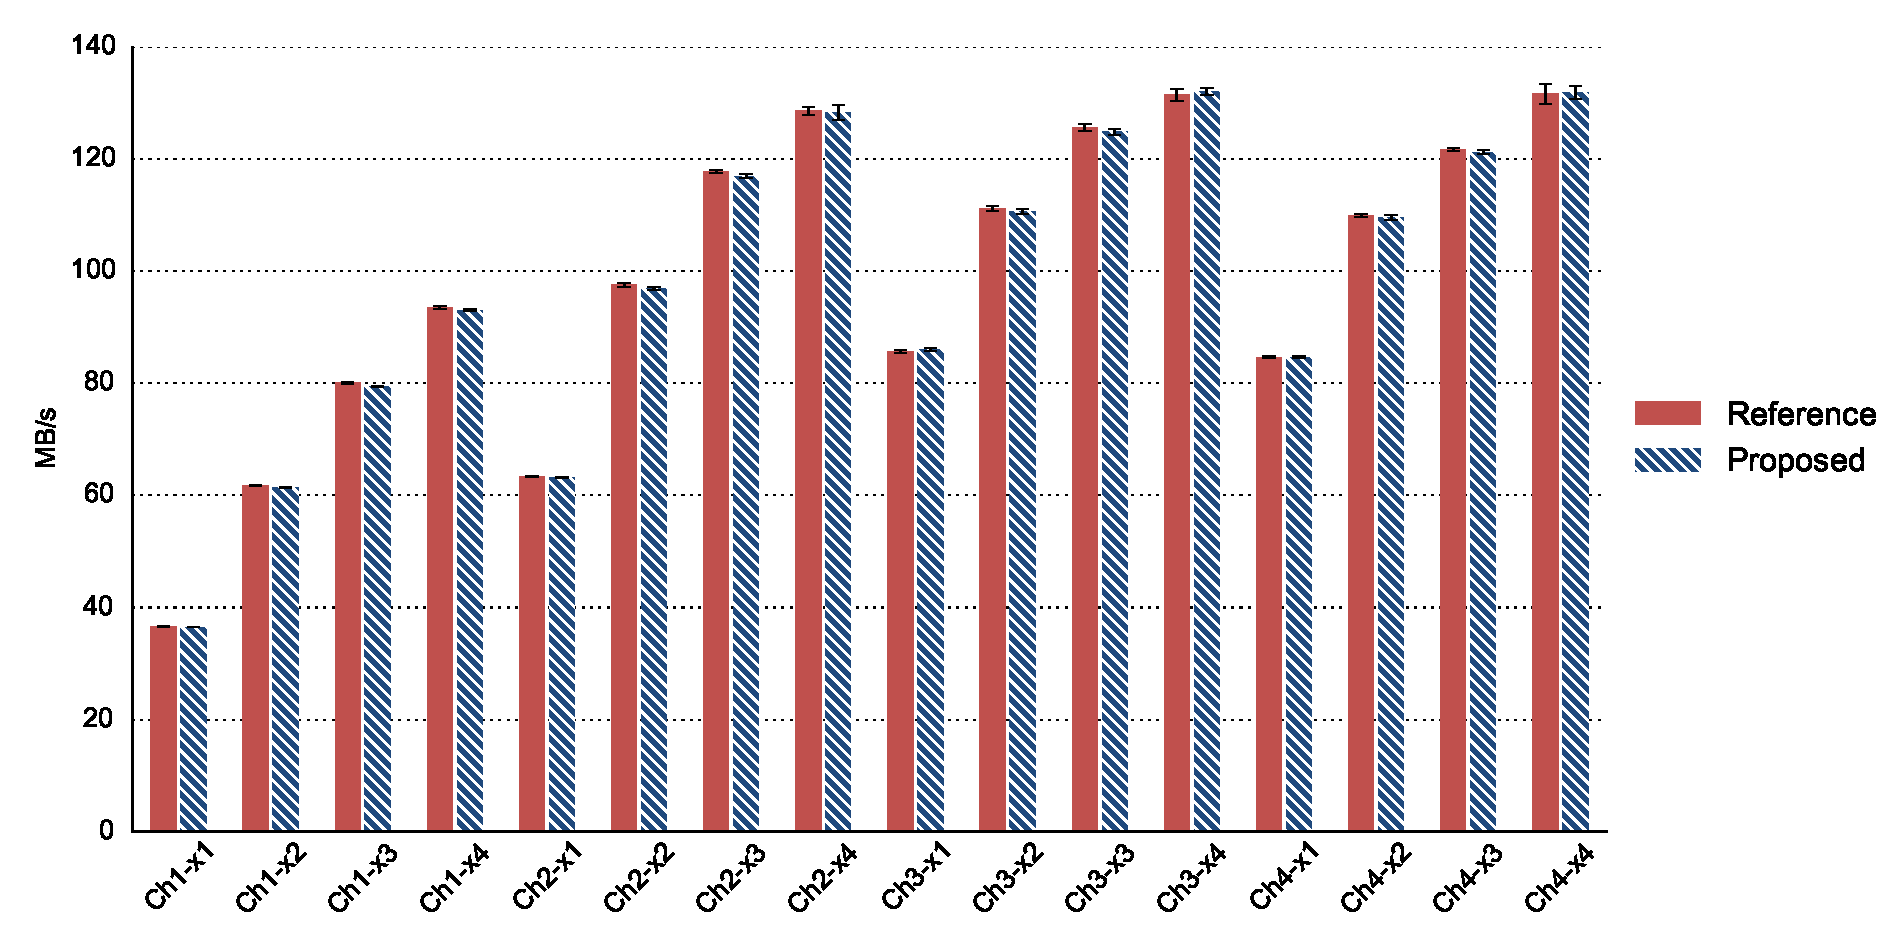
\includegraphics[width=\textwidth]{figures/ch6-fig-9.pdf}
	\caption[Sequential read bandwidth.]{\label{fig:ch6-fig-9}Sequential read bandwidth. Error bars represent the 95\% confidence intervals of the means.}
\end{figure}

\begin{table}[htbp]%
	\centering
	\caption{Frequency of disk model rollback operations for the sequential read workload}\label{tab:ch6-5-rollback}
	\noindent\begin{tabular}{cc}
		\toprule
		Storage device configuration &
		Percentage of I/Os causing rollbacks \\
		\midrule
		Ch1-x1 & 0\% \\
		Ch1-x2 & 0\% \\
		Ch1-x3 & 0\% \\
		Ch1-x4 & 0\% \\
		Ch2-x1 & 49\% \\
		Ch2-x2 & 49\% \\
		Ch2-x3 & 49\% \\
		Ch2-x4 & 49\% \\
		Ch3-x1 & 85\% \\
		Ch3-x2 & 64\% \\
		Ch3-x3 & 63\% \\
		Ch3-x4 & 49\% \\
		Ch4-x1 & 73\% \\
		Ch4-x2 & 74\% \\
		Ch4-x3 & 62\% \\
		Ch4-x4 & 49\% \\
		\bottomrule
	\end{tabular}
\end{table}%

In the first test, the sequential read bandwidth of the emulated storage device is measured using the \textit{hdparm} utility. The I/O scheduler for the emulated storage device is set to the NOOP scheduler. Setting the NOOP I/O scheduler disables the anticipatory I/O scheduling behavior that would otherwise be performed by the default I/O scheduler in the Linux kernel. With anticipatory I/O scheduling disabled, the read requests generated by the \textit{hdparm} utility will be submitted to the emulated storage device as soon as they are created. The measured results are listed in Table~\ref{tab:ch6-5} and graphed in Figure~\ref{fig:ch6-fig-9}. All results from the proposed storage device emulator are within 1\% differences to the results from the reference system. The percentage of all the I/O requests that will cause disk model simulation time rollbacks are listed in Table~\ref{tab:ch6-5-rollback}  


\subsection{The Postmark Benchmark}
\label{sec:ch6-6.6.2}

\begin{table}[htbp]%
	\small
	\begin{center}
	\caption{Elapsed time of the postmark workload}\label{tab:ch6-6}
	\hspace*{-10cm}
	\noindent\begin{tabular}{
			l
			S[table-format=3.3]
			S[table-format=3.3]
			S[table-format=3.3]
			S[table-format=3.3]
			S[table-format=3.3]
			S[table-format=3.3]
			S[table-format=1.2]
			S[table-format=1.2]
			r}
		\toprule
		{Test Config} & {Mean} & {Median} & {Low} & {High} & {Min} & {Max} & {SDEV\%} & {HW\%} & \multicolumn{1}{c}{Diff} \\
		\midrule
		
Ch1-x1 Ref. & 179.866  & 179.670  & 179.327  & 180.406  & 179.375  & 180.416  & 0.24  & 0.30 & \\
Ch1-x1 & 176.830  & 177.071  & 175.859  & 177.802  & 175.797  & 177.778  & 0.44  & 0.55 & -1.69\% \\
Ch1-x2 Ref. & 88.943  & 88.714  & 87.955  & 89.931  & 88.005  & 90.050  & 0.89  & 1.11 & \\
Ch1-x2 & 87.756  & 87.881  & 87.196  & 88.317  & 87.053  & 88.205  & 0.51  & 0.64 & -1.33\% \\
Ch1-x3 Ref. & 58.399  & 58.273  & 57.949  & 58.850  & 58.096  & 58.991  & 0.62  & 0.77 & \\
Ch1-x3 & 57.940  & 58.198  & 57.176  & 58.705  & 56.858  & 58.323  & 1.06  & 1.32 & -0.79\% \\
Ch1-x4 Ref. & 42.136  & 42.130  & 41.809  & 42.462  & 41.770  & 42.514  & 0.63  & 0.78 & \\
Ch1-x4 & 42.322  & 42.224  & 41.894  & 42.750  & 41.903  & 42.738  & 0.82  & 1.01 & 0.44\% \\
Ch2-x1 Ref. & 90.294  & 90.327  & 89.402  & 91.187  & 89.557  & 91.221  & 0.80  & 0.99 & \\
Ch2-x1 & 90.647  & 90.921  & 89.268  & 92.026  & 89.032  & 91.840  & 1.23  & 1.52 & 0.39\% \\
Ch2-x2 Ref. & 44.016  & 43.910  & 43.687  & 44.345  & 43.769  & 44.383  & 0.60  & 0.75 & \\
Ch2-x2 & 43.842  & 43.847  & 43.333  & 44.351  & 43.429  & 44.324  & 0.94  & 1.16 & -0.39\% \\
Ch2-x3 Ref. & 28.287  & 28.243  & 28.128  & 28.447  & 28.156  & 28.481  & 0.45  & 0.56 & \\
Ch2-x3 & 28.313  & 28.311  & 28.111  & 28.516  & 28.110  & 28.488  & 0.58  & 0.72 & 0.09\% \\
Ch2-x4 Ref. & 21.451  & 21.478  & 21.352  & 21.551  & 21.340  & 21.547  & 0.37  & 0.46 & \\
Ch2-x4 & 21.392  & 21.348  & 21.248  & 21.535  & 21.305  & 21.581  & 0.54  & 0.67 & -0.28\% \\
Ch3-x1 Ref. & 60.453  & 60.547  & 59.501  & 61.405  & 59.662  & 61.429  & 1.27  & 1.58 & \\
Ch3-x1 & 60.735  & 60.521  & 60.238  & 61.233  & 60.405  & 61.201  & 0.66  & 0.82 & 0.47\% \\
Ch3-x2 Ref. & 28.839  & 28.881  & 28.497  & 29.180  & 28.533  & 29.163  & 0.95  & 1.18 & \\
Ch3-x2 & 29.006  & 28.935  & 28.812  & 29.199  & 28.900  & 29.273  & 0.54  & 0.67 & 0.58\% \\
Ch3-x3 Ref. & 18.888  & 18.853  & 18.776  & 19.000  & 18.827  & 19.042  & 0.48  & 0.59 & \\
Ch3-x3 & 18.965  & 18.905  & 18.800  & 19.130  & 18.869  & 19.186  & 0.70  & 0.87 & 0.41\% \\
Ch3-x4 Ref. & 14.267  & 14.262  & 14.222  & 14.311  & 14.225  & 14.320  & 0.25  & 0.31 & \\
Ch3-x4 & 14.212  & 14.207  & 14.144  & 14.280  & 14.139  & 14.293  & 0.39  & 0.48 & -0.38\% \\
Ch4-x1 Ref. & 47.027  & 47.050  & 46.817  & 47.236  & 46.808  & 47.198  & 0.36  & 0.45 & \\
Ch4-x1 & 47.005  & 46.949  & 46.504  & 47.506  & 46.471  & 47.444  & 0.86  & 1.07 & -0.05\% \\
Ch4-x2 Ref. & 21.997  & 22.012  & 21.821  & 22.173  & 21.854  & 22.200  & 0.64  & 0.80 & \\
Ch4-x2 & 22.027  & 22.039  & 21.933  & 22.120  & 21.932  & 22.121  & 0.34  & 0.42 & 0.14\% \\
Ch4-x3 Ref. & 14.245  & 14.227  & 14.184  & 14.306  & 14.195  & 14.324  & 0.35  & 0.43 & \\
Ch4-x3 & 14.330  & 14.312  & 14.246  & 14.413  & 14.268  & 14.419  & 0.47  & 0.58 & 0.60\% \\
Ch4-x4 Ref. & 10.809  & 10.807  & 10.760  & 10.859  & 10.762  & 10.850  & 0.37  & 0.46 & \\
Ch4-x4 & 10.806  & 10.821  & 10.711  & 10.902  & 10.689  & 10.900  & 0.71  & 0.88 & -0.03\% \\

		\bottomrule
	\end{tabular}
	\hspace*{-10cm}
	\end{center}
	
	Remarks: Units are in 100 seconds. Low and high are the Student-\textit{t} confidence interval error bar values. SDEV\% and HW\% are the standard deviation and half-width of the confidence interval as a percent of the mean.
\end{table}%



\begin{figure}[htpb]
	\centering
	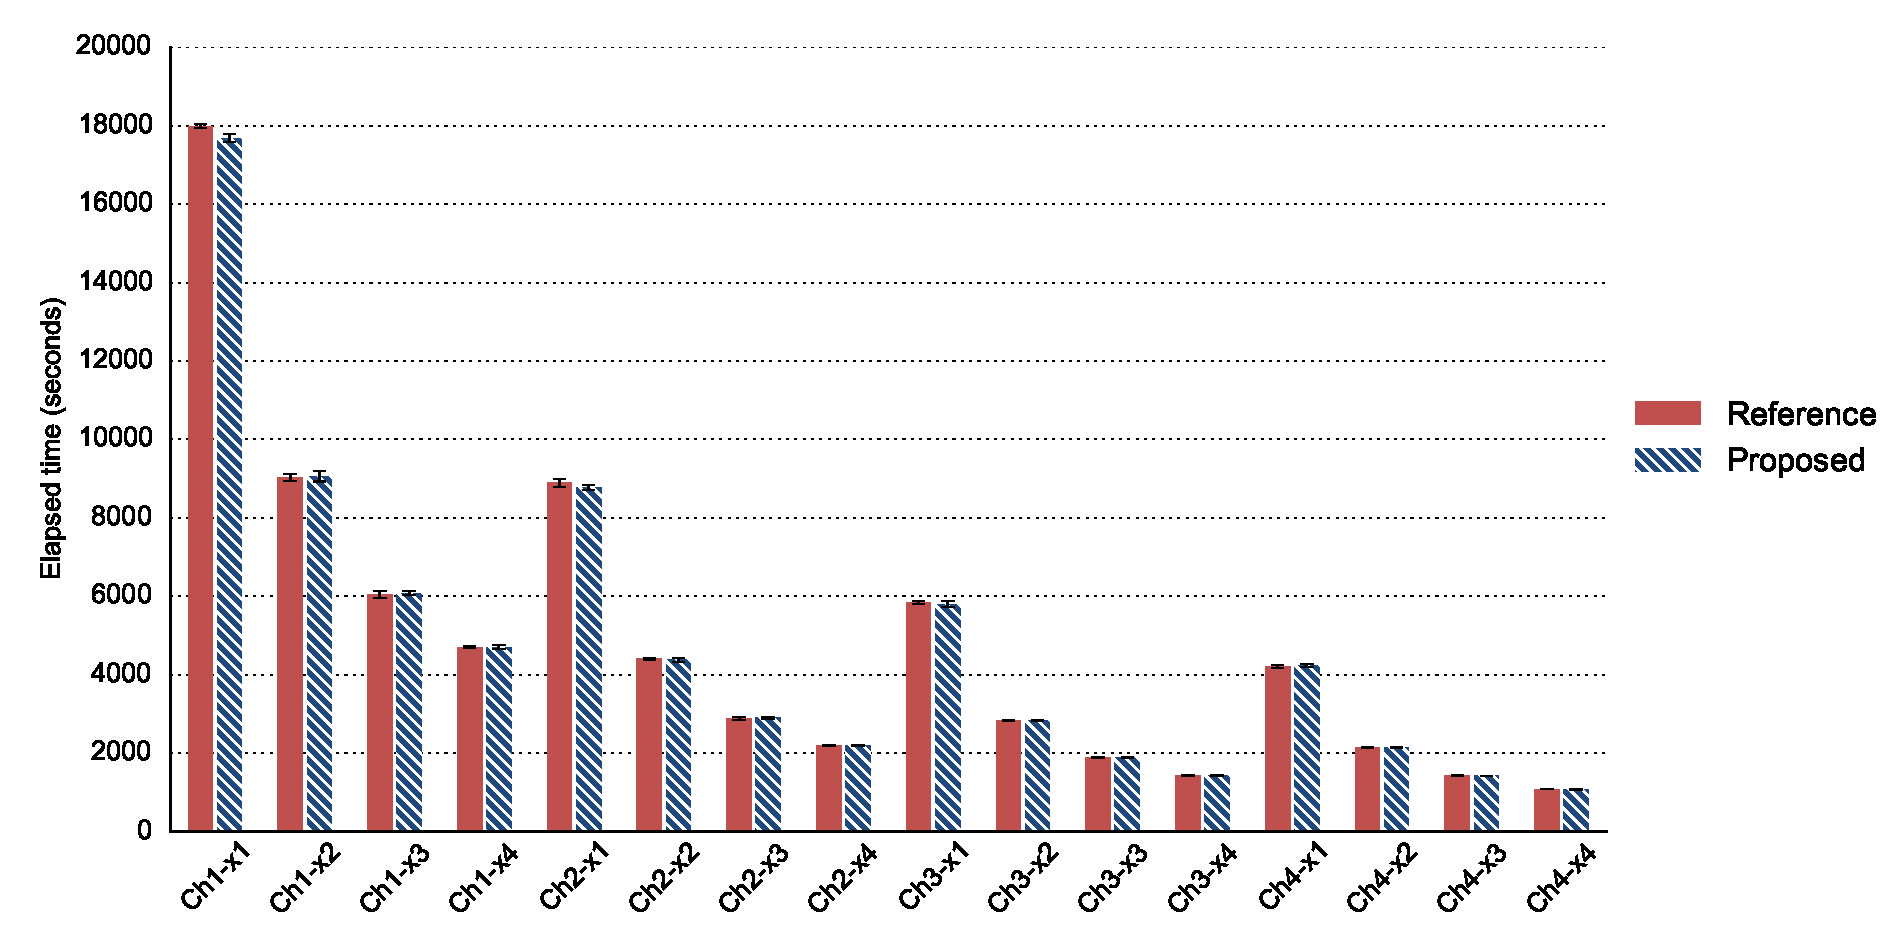
\includegraphics[width=\textwidth]{figures/ch6-fig-10.pdf}
	\caption[Elapsed time of the postmark workload.]{\label{fig:ch6-fig-10}Elapsed time of the postmark workload. Error bars represent the 95\% confidence intervals of the means.}
\end{figure}

\begin{table}[htbp]%
	\centering
	\caption{Frequency of disk model rollback operations for the postmark workload}\label{tab:ch6-6-rollback}
	\noindent\begin{tabular}{cc}
		\toprule
		Storage device configuration &
		Percentage of I/Os causing rollbacks \\
		\midrule
		Ch1-x1 & 0\% \\
		Ch1-x2 & 0\% \\
		Ch1-x3 & 0\% \\
		Ch1-x4 & 0\% \\
		Ch2-x1 & 96\% \\
		Ch2-x2 & 91\% \\
		Ch2-x3 & 87\% \\
		Ch2-x4 & 80\% \\
		Ch3-x1 & 97\% \\
		Ch3-x2 & 91\% \\
		Ch3-x3 & 85\% \\
		Ch3-x4 & 81\% \\
		Ch4-x1 & 95\% \\
		Ch4-x2 & 90\% \\
		Ch4-x3 & 86\% \\
		Ch4-x4 & 81\% \\
		\bottomrule
	\end{tabular}
\end{table}%

The postmark workload is used as the next set of workloads for validation. The ext3 file system is created on the emulated storage device and both scenarios for the NOOP I/O scheduler and the CFQ I/O scheduler are tested. To test how the proposed storage emulator works under multithreaded environment, 8 concurrent postmark threads are used to generate a total of 100,000 transactions over a set of 10,000 files. Each postmark thread will generate 12,500 transactions. All results from the proposed storage device emulator are within 2\% differences to the results from the reference system. The evaluation results for the CFQ I/O scheduler are listed in Table~\ref{tab:ch6-6} and graphed in Figure~\ref{fig:ch6-fig-10}. The percentage of all the I/O requests that will cause disk model simulation time rollbacks are listed in Table~\ref{tab:ch6-6-rollback}  

To give an idea of the I/O patterns generated by the above postmark setup, the the randomness of the generated workloads are measured and listed in Table~\ref{tab:ch6-postmark-randomness}.

\begin{table}[htbp]%
	\centering
	\caption{I/O request randomness of the postmark workload}\label{tab:ch6-postmark-randomness}
	\noindent\begin{tabular}{ccc}
		\toprule
		&\multicolumn{2}{c}{Percentage of random I/O requests}\\
		\cmidrule(lr){2-3}
		\parbox{3cm}{\centering Storage device \\ configuration} &
		\parbox{4cm}{\centering with the CFQ\\I/O scheduler}&
		\parbox{4cm}{\centering with the NOOP\\I/O scheduler}\\
		
		\midrule
		Ch1-x1 & 97.23\% & 96.76\% \\
		Ch1-x2 & 97.26\% & 96.61\% \\
		Ch1-x3 & 96.96\% & 96.83\% \\
		Ch1-x4 & 96.84\% & 96.79\% \\
		Ch2-x1 & 96.07\% & 96.43\% \\
		Ch2-x2 & 96.24\% & 96.27\% \\
		Ch2-x3 & 96.38\% & 96.53\% \\
		Ch2-x4 & 96.36\% & 96.84\% \\
		Ch3-x1 & 95.98\% & 96.46\% \\
		Ch3-x2 & 96.35\% & 96.47\% \\
		Ch3-x3 & 96.56\% & 96.95\% \\
		Ch3-x4 & 96.92\% & 97.20\% \\
		Ch4-x1 & 96.16\% & 96.17\% \\
		Ch4-x2 & 96.35\% & 96.74\% \\
		Ch4-x3 & 96.88\% & 97.15\% \\
		Ch4-x4 & 97.29\% & 97.44\% \\
		\bottomrule
	\end{tabular}
\end{table}%


\subsection{Linux Kernel Source Archive Extraction and Word Count}
\label{sec:ch6-6.6.3}

\begin{table}[htbp]%
	\small
	\begin{center}
	\caption{Elapsed time of Linux kernel source archive extraction and word count}\label{tab:ch6-7}
	\hspace*{-2cm}
	\noindent\begin{tabular}{
			l
			S[table-format=3.2]
			S[table-format=3.2]
			S[table-format=3.2]
			S[table-format=3.2]
			S[table-format=3.2]
			S[table-format=3.2]
			S[table-format=1.2]
			S[table-format=1.2]
			r}
		\toprule
		{Test Config} & {Mean} & {Median} & {Low} & {High} & {Min} & {Max} & {SDEV\%} & {HW\%} & \multicolumn{1}{c}{Diff} \\
		\midrule
		
		Ch1-x1 Ref. & 335.17  & 332.95  & 330.27  & 340.07  & 326.38  & 345.15  & 2.05  & 1.46 & \\
		Ch1-x1 & 328.92  & 326.83  & 322.97  & 334.87  & 318.08  & 340.87  & 2.53  & 1.81 & -1.87\% \\
		Ch1-x2 Ref. & 186.27  & 185.40  & 183.38  & 189.16  & 180.34  & 193.04  & 2.17  & 1.55 & \\
		Ch1-x2 & 188.25  & 188.01  & 184.41  & 192.09  & 181.40  & 196.96  & 2.85  & 2.04 & 1.06\% \\
		Ch1-x3 Ref. & 162.22  & 162.04  & 159.98  & 164.46  & 157.74  & 166.61  & 1.93  & 1.38 & \\
		Ch1-x3 & 162.99  & 162.34  & 161.03  & 164.94  & 160.48  & 169.43  & 1.67  & 1.20 & 0.47\% \\
		Ch1-x4 Ref. & 153.93  & 152.34  & 150.26  & 157.60  & 148.39  & 176.21  & 4.31  & 2.38 & \\
		Ch1-x4 & 152.83  & 152.94  & 151.76  & 153.91  & 150.48  & 155.58  & 0.98  & 0.70 & -0.71\% \\	
		Ch2-x1 Ref. & 184.21  & 184.49  & 181.03  & 187.39  & 177.93  & 189.77  & 2.41  & 1.73 & \\
		Ch2-x1 & 181.93  & 179.86  & 177.68  & 186.19  & 174.86  & 195.40  & 3.68  & 2.34 & -1.24\% \\
		Ch2-x2 Ref. & 154.29  & 154.44  & 152.46  & 156.12  & 150.05  & 158.18  & 1.66  & 1.19  & \\
		Ch2-x2 & 154.92  & 154.82  & 153.40  & 156.43  & 150.73  & 157.40  & 1.37  & 0.98 & 0.41\% \\
		Ch2-x3 Ref. & 147.60  & 147.55  & 146.88  & 148.32  & 145.86  & 149.25  & 0.68  & 0.49 & \\
		Ch2-x3 & 148.38  & 148.30  & 147.79  & 148.97  & 147.47  & 150.30  & 0.56  & 0.40 & 0.53\% \\
		Ch2-x4 Ref. & 145.95  & 145.97  & 145.47  & 146.43  & 145.26  & 147.49  & 0.46  & 0.33 & \\
		Ch2-x4 & 146.22  & 146.18  & 145.62  & 146.82  & 145.01  & 147.74  & 0.58  & 0.41 & 0.18\% \\
		Ch3-x1 Ref. & 171.05  & 171.03  & 166.87  & 175.22  & 163.22  & 186.23  & 3.63  & 2.44 & \\
		Ch3-x1 & 171.69  & 172.34  & 168.09  & 175.29  & 163.12  & 178.03  & 2.93  & 2.10 & 0.38\% \\
		Ch3-x2 Ref. & 152.70  & 152.25  & 151.49  & 153.90  & 150.39  & 155.78  & 1.10  & 0.79 & \\
		Ch3-x2 & 152.44  & 151.74  & 150.93  & 153.95  & 150.13  & 156.69  & 1.38  & 0.99 & -0.17\% \\
		Ch3-x3 Ref. & 146.66  & 146.68  & 146.30  & 147.03  & 145.75  & 147.62  & 0.35  & 0.25 & \\
		Ch3-x3 & 147.15  & 147.37  & 146.64  & 147.67  & 145.63  & 148.05  & 0.49  & 0.35 & 0.33\% \\
		Ch3-x4 Ref. & 145.67  & 145.55  & 145.36  & 145.98  & 144.97  & 146.46  & 0.30  & 0.21 & \\
		Ch3-x4 & 145.52  & 145.37  & 145.30  & 145.74  & 145.21  & 146.00  & 0.21  & 0.15 & -0.10\% \\
		Ch4-x1 Ref. & 168.66  & 167.48  & 166.15  & 171.17  & 164.61  & 175.39  & 2.08  & 1.49 & \\
		Ch4-x1 & 166.84  & 167.60  & 164.74  & 168.94  & 162.15  & 171.77  & 1.76  & 1.26 & -1.08\% \\
		Ch4-x2 Ref. & 151.06  & 151.01  & 150.17  & 151.95  & 148.62  & 152.84  & 0.82  & 0.59 & \\
		Ch4-x2 & 152.65  & 151.96  & 150.70  & 154.60  & 148.67  & 157.48  & 1.79  & 1.28 & 1.05\% \\
		Ch4-x3 Ref. & 146.33  & 146.45  & 146.00  & 146.67  & 145.58  & 147.05  & 0.32  & 0.23 & \\
		Ch4-x3 & 146.86  & 146.91  & 146.23  & 147.48  & 145.44  & 148.02  & 0.59  & 0.42 & 0.36\% \\
		Ch4-x4 Ref. & 145.01  & 145.13  & 144.71  & 145.31  & 144.27  & 145.64  & 0.29  & 0.20 & \\
		Ch4-x4 & 145.53  & 145.32  & 144.97  & 146.09  & 144.57  & 146.78  & 0.54  & 0.38 & 0.36\% \\
		
		\bottomrule
	\end{tabular}
	\hspace*{-2cm}
	\end{center}
	
	Remarks: Units are in seconds. Low and high are the Student-\textit{t} confidence interval error bar values. SDEV\% and HW\% are the standard deviation and half-width of the confidence interval as a percent of the mean.
\end{table}%

\begin{figure}[htpb]
	\centering
	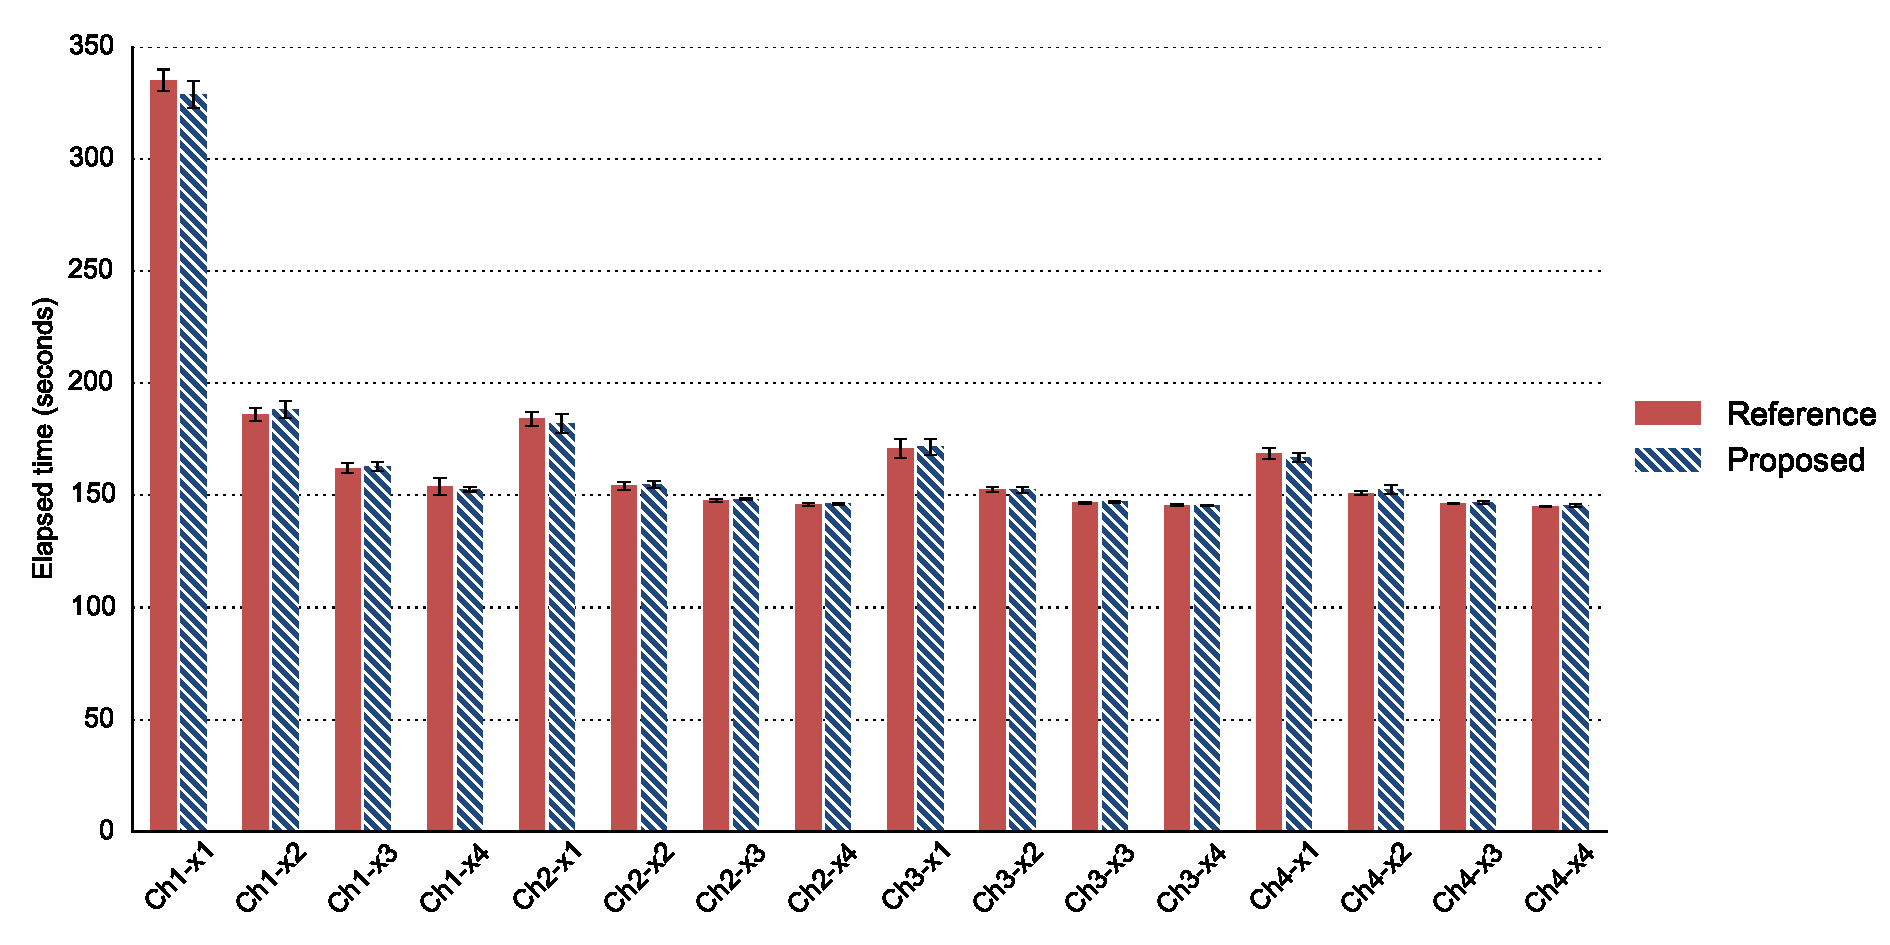
\includegraphics[width=\textwidth]{figures/ch6-fig-11.pdf}
	\caption[Elapsed time of Linux kernel source archive extraction and word count.]{\label{fig:ch6-fig-11}Elapsed time of Linux kernel source archive extraction and word count. Error bars represent the 95\% confidence intervals of the means.}
\end{figure}

\begin{table}[htbp]%
	\centering
	\caption{Frequency of disk model rollback operations for the Linux kernel source archive extraction and work count workload}\label{tab:ch6-7-rollback}
	\noindent\begin{tabular}{cc}
		\toprule
		Storage device configuration &
		Percentage of I/Os causing rollbacks \\
		\midrule
		Ch1-x1 & 0\% \\
		Ch1-x2 & 0\% \\
		Ch1-x3 & 0\% \\
		Ch1-x4 & 0\% \\
		Ch2-x1 & 96\% \\
		Ch2-x2 & 91\% \\
		Ch2-x3 & 87\% \\
		Ch2-x4 & 80\% \\
		Ch3-x1 & 97\% \\
		Ch3-x2 & 91\% \\
		Ch3-x3 & 85\% \\
		Ch3-x4 & 81\% \\
		Ch4-x1 & 95\% \\
		Ch4-x2 & 90\% \\
		Ch4-x3 & 86\% \\
		Ch4-x4 & 81\% \\
		\bottomrule
	\end{tabular}
\end{table}%

Besides using synthetic workloads, the proposed storage device emulator is also validated using real application programs. In this test, the ext4 file system is created on the emulated storage device and both scenarios for the NOOP I/O scheduler and the CFQ I/O scheduler are tested. The Linux kernel source archive (linux-3.10.tar.bz2) downloaded from kernel.org~\cite{Kernel:2013:3.10source} is first copied to the ext4 file system and then extracted in place. Table~\ref{tab:ch6-linux-archive} lists the information about the size and the number of files for the top level directories in the archive. The percentage of all the I/O requests that will cause disk model simulation time rollbacks are listed in Table~\ref{tab:ch6-7-rollback}  


\begin{table}[htbp]%
	\small
	\begin{center}
		\caption{Contents of the Linux kernel source archive}\label{tab:ch6-linux-archive}
		\noindent\begin{tabular}{lrr}
		\toprule

		Directory name & Content size & Number of files \\
		\midrule
		./init & 180KB & 13 \\
		./net & 23M & 1417 \\
		./Documentation & 24M & 2581 \\
		./samples & 204K & 34 \\
		./usr & 40K & 5 \\
		./ipc & 240K & 15 \\
		./arch & 126M & 15497 \\
		./virt & 216K & 14 \\
		./security & 2.2M & 169 \\
		./crypto & 2.5M & 113 \\
		./scripts & 2.7M & 250 \\
		./firmware & 6.0M & 151 \\
		./tools & 5.2M & 616 \\
		./block & 912K & 64 \\
		./fs & 35M & 1726 \\
		./sound & 26M & 1434 \\
		./kernel & 5.8M & 273 \\
		./drivers & 283M & 14824 \\
		./lib & 2.1M & 234 \\
		./include & 27M & 3493 \\
		./mm & 2.7M & 83 \\		
		\bottomrule
		\end{tabular}
	\end{center}
\end{table}%

Because the total size of the entire working set will be over 400MB, the contents under the Documentation and the drivers directories in the source archive are omitted. After extraction, the total number of words in the source files is then counted using the wc utility. The total elapsed time for extracting the kernel achieve and performing the word count is measured. All results from the proposed storage device emulator are within 2\% differences to the results from the reference system. The measured results for the CFQ I/O scheduler are listed in Table~\ref{tab:ch6-7} and graphed in Figure~\ref{fig:ch6-fig-11}.

This test scenario highlights a limitation of the reference local emulation type emulator: the size of the storage device that can be emulated is limited to the size of the available memory which can be used as the backing storage. In this test, the Documentation and the drivers directories in the kernel source archive need to be omitted so that the total working set will fit into the 400MB storage device. In comparison, the proposed storage device emulator does not have this kind of limitation. The size of the storage device that can be emulated by the proposed storage device emulator can be as large as the backing storage available on the emulator server. Moreover, because the state of the OS is paused while the backing storage is being accessed, the performance evaluation results will not be affected by the speed of the backing storage used. This means that slower backing storages can be used for emulating faster storage devices. In our experiments, the backing storage device used by the proposed storage device emulator is a traditional hard disk drive, and the proposed storage device emulator have no problem using it for emulating storage devices that have sub-millisecond response times.


\subsection{Video Encoding and Decoding}
\label{sec:ch6-6.6.4}

\begin{table}[htbp]%
	\small
	\begin{center}
	\caption[Elapsed time of MPEG2 video encoding and decoding]{Elapsed time of MPEG2 video encoding and decoding the CIF resolution \textit{foreman} sequence}\label{tab:ch6-8}
	\hspace*{-2cm}
	\noindent\begin{tabular}{
			l
			S[table-format=2.2]
			S[table-format=2.2]
			S[table-format=2.2]
			S[table-format=2.2]
			S[table-format=2.2]
			S[table-format=2.2]
			S[table-format=1.2]
			S[table-format=1.2]
			r}
		\toprule
		{Test Config} & {Mean} & {Median} & {Low} & {High} & {Min} & {Max} & {SDEV\%} & {HW\%} & \multicolumn{1}{c}{Diff} \\
		\midrule
		
Ch1-x1 Ref. & 12.48  & 12.55  & 12.33  & 12.64  & 12.22  & 12.83  & 1.76  & 1.26 & \\
Ch1-x1 & 12.57  & 12.64  & 12.39  & 12.74  & 12.23  & 12.84  & 1.94  & 1.39 & 0.67\% \\
Ch1-x2 Ref. & 8.56  & 8.56  & 8.49  & 8.63  & 8.43  & 8.68  & 1.14  & 0.82 & \\
Ch1-x2 & 8.56  & 8.54  & 8.50  & 8.62  & 8.47  & 8.69  & 0.97  & 0.70 & -0.06\% \\
Ch1-x3 Ref. & 7.22  & 7.24  & 7.20  & 7.25  & 7.15  & 7.27  & 0.55  & 0.39 & \\
Ch1-x3 & 7.22  & 7.23  & 7.16  & 7.27  & 7.09  & 7.36  & 1.07  & 0.77 & -0.10\% \\
Ch1-x4 Ref. & 6.72  & 6.68  & 6.66  & 6.77  & 6.64  & 6.83  & 1.12  & 0.80 & \\
Ch1-x4 & 6.66  & 6.66  & 6.63  & 6.69  & 6.59  & 6.71  & 0.62  & 0.44 & -0.83\% \\
Ch2-x1 Ref. & 8.98  & 8.98  & 8.83  & 9.14  & 8.47  & 9.28  & 2.48  & 1.77 & \\
Ch2-x1 & 8.94  & 8.93  & 8.75  & 9.14  & 8.44  & 9.32  & 3.07  & 2.20 & -0.47\% \\
Ch2-x2 Ref. & 7.00  & 7.02  & 6.92  & 7.09  & 6.78  & 7.21  & 1.77  & 1.26 & \\
Ch2-x2 & 6.91  & 6.94  & 6.80  & 7.01  & 6.69  & 7.15  & 2.11  & 1.51 & -1.38\% \\
Ch2-x3 Ref. & 6.48  & 6.50  & 6.44  & 6.53  & 6.37  & 6.56  & 0.94  & 0.67 & \\
Ch2-x3 & 6.48  & 6.47  & 6.42  & 6.53  & 6.35  & 6.57  & 1.10  & 0.79 & -0.14\% \\
Ch2-x4 Ref. & 6.31  & 6.32  & 6.29  & 6.34  & 6.26  & 6.36  & 0.51  & 0.37 & \\
Ch2-x4 & 6.32  & 6.31  & 6.29  & 6.35  & 6.25  & 6.38  & 0.63  & 0.45 & 0.08\% \\
Ch3-x1 Ref. & 8.08  & 8.11  & 7.89  & 8.28  & 7.58  & 8.69  & 4.02  & 2.43 & \\
Ch3-x1 & 8.14  & 8.10  & 7.94  & 8.33  & 7.69  & 8.76  & 3.93  & 2.37 & 0.67\% \\
Ch3-x2 Ref. & 6.80  & 6.80  & 6.76  & 6.85  & 6.68  & 6.87  & 0.95  & 0.68 & \\
Ch3-x2 & 6.79  & 6.80  & 6.72  & 6.87  & 6.58  & 6.92  & 1.51  & 1.08 & -0.15\% \\
Ch3-x3 Ref. & 6.40  & 6.40  & 6.37  & 6.43  & 6.30  & 6.47  & 0.72  & 0.52 & \\
Ch3-x3 & 6.39  & 6.37  & 6.35  & 6.42  & 6.31  & 6.44  & 0.71  & 0.51 & -0.20\% \\
Ch3-x4 Ref. & 6.23  & 6.23  & 6.21  & 6.25  & 6.17  & 6.27  & 0.48  & 0.34 & \\
Ch3-x4 & 6.22  & 6.24  & 6.18  & 6.26  & 6.09  & 6.30  & 0.91  & 0.65 & -0.11\% \\
Ch4-x1 Ref. & 7.84  & 7.84  & 7.73  & 7.95  & 7.65  & 8.09  & 1.91  & 1.37 & \\
Ch4-x1 & 7.83  & 7.87  & 7.65  & 8.01  & 7.22  & 8.18  & 3.63  & 2.31 & -0.15\% \\
Ch4-x2 Ref. & 6.69  & 6.70  & 6.65  & 6.73  & 6.61  & 6.77  & 0.82  & 0.58 & \\
Ch4-x2 & 6.63  & 6.61  & 6.57  & 6.69  & 6.51  & 6.74  & 1.19  & 0.85 & -0.88\% \\
Ch4-x3 Ref. & 6.33  & 6.33  & 6.31  & 6.35  & 6.29  & 6.37  & 0.45  & 0.32 & \\
Ch4-x3 & 6.34  & 6.35  & 6.30  & 6.38  & 6.25  & 6.41  & 0.83  & 0.59 & 0.11\% \\
Ch4-x4 Ref. & 6.14  & 6.15  & 6.12  & 6.15  & 6.10  & 6.16  & 0.36  & 0.26 & \\
Ch4-x4 & 6.17  & 6.18  & 6.15  & 6.19  & 6.10  & 6.20  & 0.45  & 0.32 & 0.57\% \\

		\bottomrule
	\end{tabular}
	\hspace*{-2cm}
	\end{center}
	
	Remarks: Units are in seconds. Low and high are the Student-\textit{t} confidence interval error bar values. SDEV\% and HW\% are the standard deviation and half-width of the confidence interval as a percent of the mean.
\end{table}%

\begin{figure}[htpb]
	\centering
	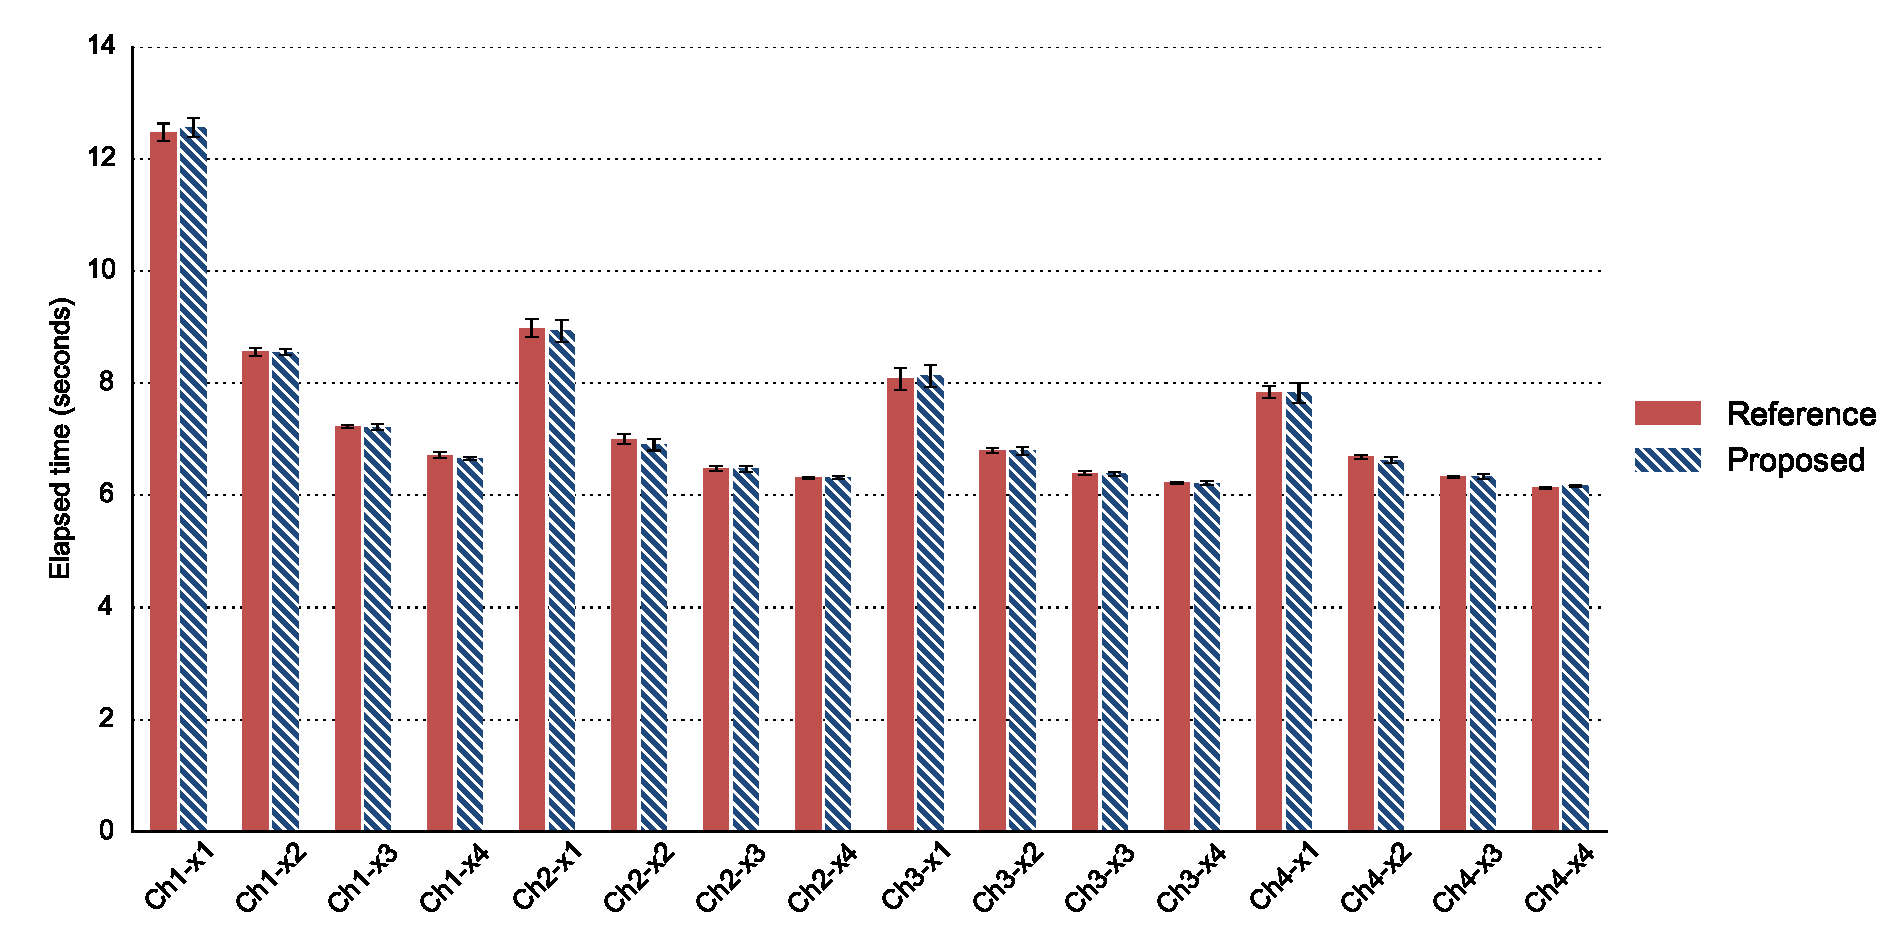
\includegraphics[width=\textwidth]{figures/ch6-fig-12.pdf}
	\caption[Elapsed time of MPEG2 video encoding and decoding.]{\label{fig:ch6-fig-12}Elapsed time of MPEG2 video encoding and decoding the CIF resolution \textit{foreman} sequence. Error bars represent the 95\% confidence intervals of the means.}
\end{figure}

\begin{table}[htbp]%
	\centering
	\caption{Frequency of disk model rollback operations for the MPEG2 video encoding and decoding workload}\label{tab:ch6-8-rollback}
	\noindent\begin{tabular}{cc}
		\toprule
		Storage device configuration &
		Percentage of I/Os causing rollbacks \\
		\midrule
		Ch1-x1 & 0\% \\
		Ch1-x2 & 0\% \\
		Ch1-x3 & 0\% \\
		Ch1-x4 & 0\% \\
		Ch2-x1 & 76\% \\
		Ch2-x2 & 72\% \\
		Ch2-x3 & 75\% \\
		Ch2-x4 & 74\% \\
		Ch3-x1 & 75\% \\
		Ch3-x2 & 75\% \\
		Ch3-x3 & 75\% \\
		Ch3-x4 & 73\% \\
		Ch4-x1 & 74\% \\
		Ch4-x2 & 78\% \\
		Ch4-x3 & 74\% \\
		Ch4-x4 & 73\% \\
		\bottomrule
	\end{tabular}
\end{table}%

In this test, the ext3 file system is created on the emulated storage device and both scenarios for the NOOP I/O scheduler and the CFQ I/O scheduler are tested. In the test, the raw CIF resolution \textit{foreman} video sequence is first copied to the ext3 file system. The raw video sequence is then encoded to the MPEG2 format using the \textit{avconv}~\cite{Libav:2014} video encoder. After encoding, the encoded MPEG2 sequence is decoded back to the raw format using the \textit{avconv} video decoder. The total elapsed time for encoding and decoding the video sequence is measured. All results from the proposed storage device emulator are within 2\% differences to the results from the reference system. The measured results are listed in Table~\ref{tab:ch6-8} and graphed in Figure~\ref{fig:ch6-fig-12}. The percentage of all the I/O requests that will cause disk model simulation time rollbacks are listed in Table~\ref{tab:ch6-8-rollback}

\subsection{Effects of Disk Model Complexity on Conventional Storage Device Emulators}

One problem with the conventional storage device emulators is that if the time it takes to simulate the disk model exceeds the response times of the corresponding I/O request, then the emulator will fail to emulate the intended behavior of the target storage device. For example, if it takes the emulator 2\si{\milli\second} to simulate the disk model for an I/O response, then the emulator will inevitably fail to properly emulate I/O responses that are supposed to be completed faster than 2\si{\milli\second}. The faster the storage device is, the more likely that the emulator will fail to emulate the correct response timings for the I/O requests. In this section, we evaluate how the amount of time needed for simulating the disk model can affect the local emulation type emulator used in the reference system.

To get a sense of how much time that a typical disk model simulator would require for simulating an I/O request, we ported the DiskSim simulator version 4.0~\cite{Bucy:2008} to ZedBoard and measured its operation speed. In our measurement, it took DiskSim approximately 37 seconds to simulate 10,000 I/O operations for a disk device. That is, the amount of time required for simulating each I/O request is about 3.7\si{\milli\second}.

To study the effect of disk model complexity on the conventional storage device emulators, we introduce artificial delays to the disk model used by the reference system to simulate disk models of different complexity. The timing delays introduced to the disk model are ranged from 0.25\si{\milli\second} to 2\si{\milli\second} in 0.25\si{\milli\second} increments. The sequential read bandwidth benchmark described in section~\ref{sec:ch6-6.6.1} is used for testing. The evaluation results are illustrated in Figure~\ref{fig:ch6-fig-13}. To save space, only the results for the single channel storage device configurations are shown. From the results, we can see that the faster the emulated storage device is, the more impact that disk model complexity will have on the reference system. For example, when emulating faster storage devices, such as the storage device with the Ch1-x4 configuration, even a disk model processing time of just 1\si{\milli\second} can affect the predicted performance by more than 50\%.

\begin{figure}[htpb]
	\centering
	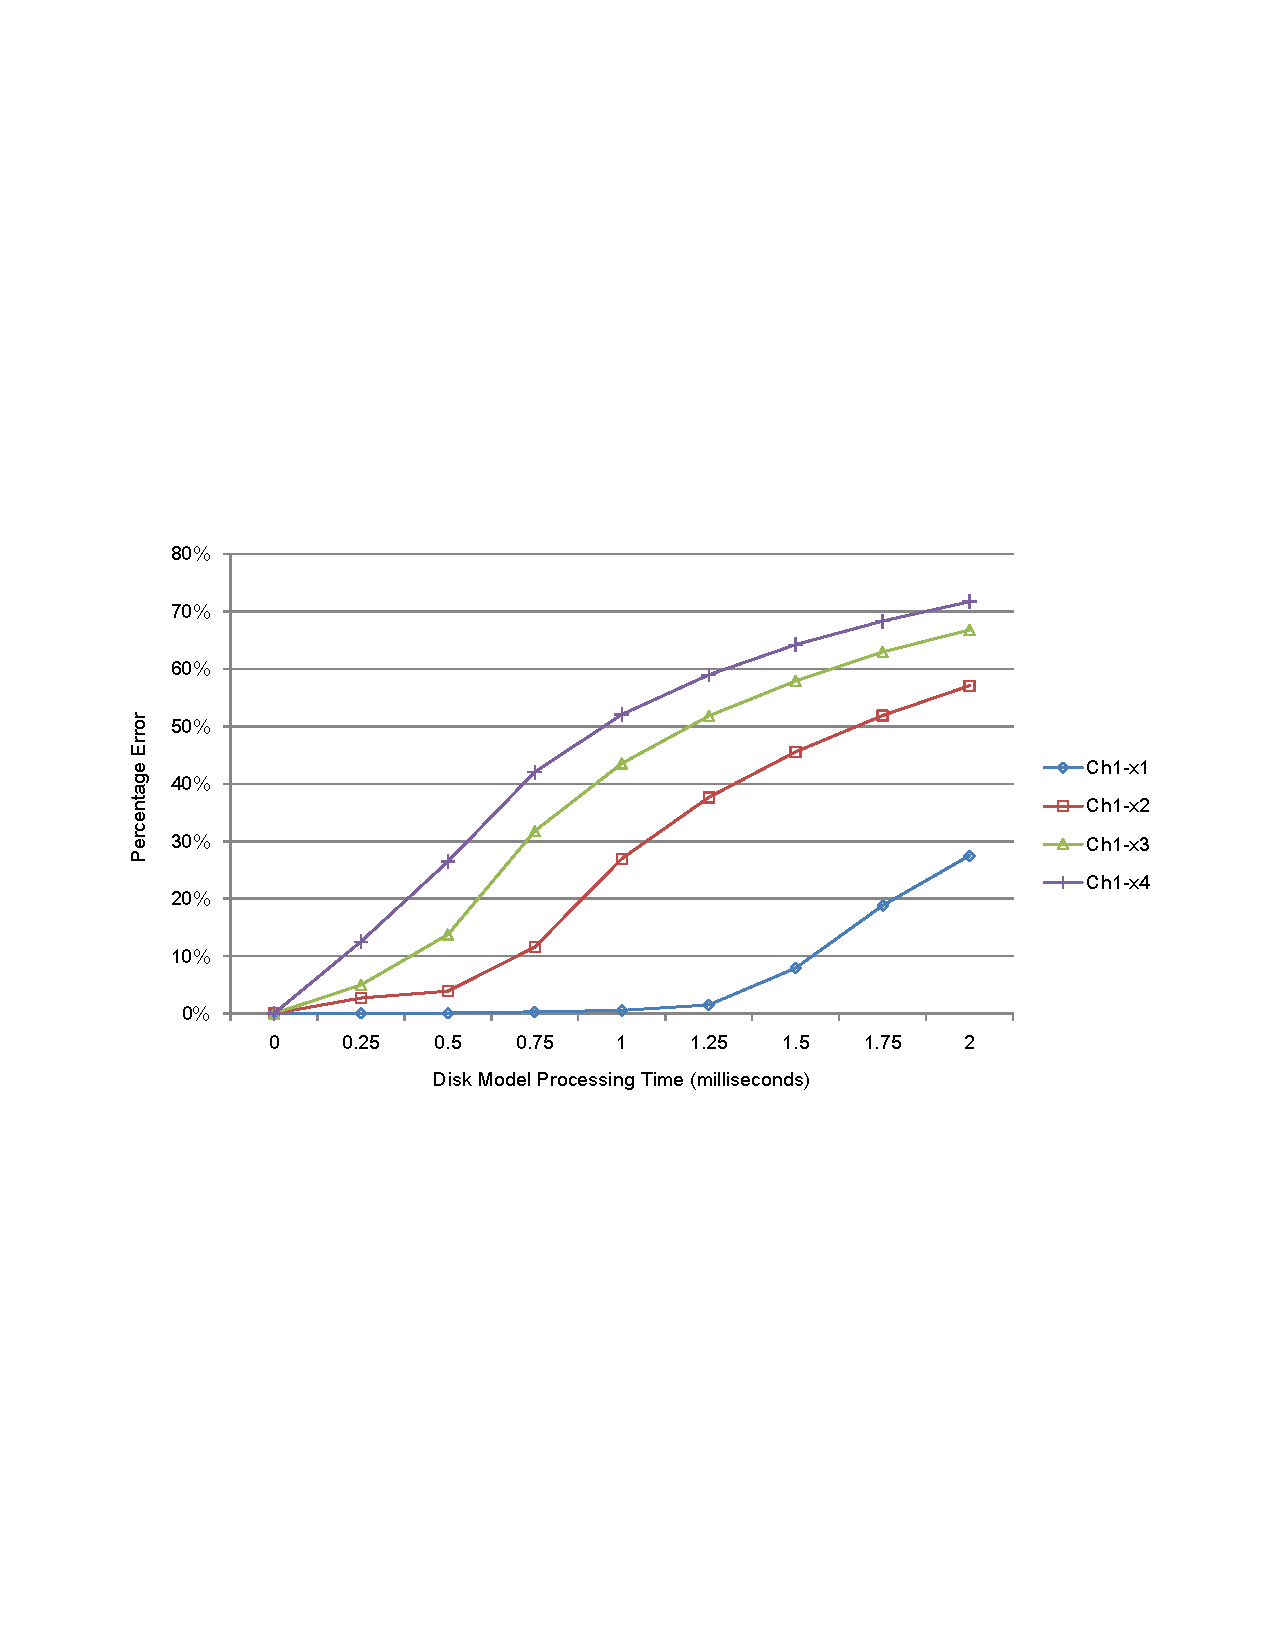
\includegraphics[trim=2cm 9.2cm 2cm 9cm, width=\textwidth]{figures/ch6-fig-13.pdf}
	\caption[Effects of disk model processing time on conventional storage device emulators.]{\label{fig:ch6-fig-13}Effects of disk model processing time on conventional storage device emulators. In conventional storage device emulators, disk model processing time can affect the characteristics of the emulated storage device and thus lead to performance evaluation errors.}
\end{figure}

In comparison, in the proposed emulator, because the OS is put into the paused state while the emulator server is simulating the disk model, the evaluation results from the proposed emulator will not be affected by the complexity of the disk model. This means that disk models of arbitrary complexity can be used in the proposed emulator for modeling complex storage device behaviors.

\chapter{Conclusions and Future Work}
\label{ch:7}

\section{Conclusions}

This dissertation describes a novel OS state pausing approach that can be used to allow OS running on real computer hardware to be co-simulated with virtually simulated storage device in the discrete-time domain. Due to reason that the co-simulation of the virtual storage device and the OS is happening in the discrete-time domain, the speed of the entire simulation process is not limited to the real-time speed. This means that: (1) When needed, the state of the OS can be frozen to wait for the processing of the virtual storage device. The storage device simulator can take as long as it needs for simulating the storage device without affecting the performance of the virtual storage device as perceived by the OS. This allows storage devices of arbitrarily speeds to be easily simulated without being constraint by the performance of the available hardware. (2) When the entire system is simply waiting in the CPU idle loop for a certain amount of time to pass by, the simulation process can be fast-forwarded to a future time point by advancing the current system time directly. This allows the simulation to be conducted at faster than real-time speeds.

Two co-simulation environments are built using the proposed co-simulation methodology. The first environment is a full-system co-simulator that allows storage subsystem equipped with simulated storage device to be evaluated using realistic workloads generated by real application programs running on real hardware. With the CPU idle loop time-skipping feature, the proposed full-system simulator is able to conduct experiments in faster than real-time speeds. Simulation speeds of up to 45$\times$ are observed in the experimental results. The second environment is a storage device emulator that allows the studying of the performance of real computer systems when different storage devices are available. Experimental results show that the performances measured using the proposed storage device emulator are within 2\% differences compared to the results from the reference system. 

\section{Directions for Future Research}

\subsection{Support for Emulating Multiple Storage Devices}

An improvement that can be made to the proposed co-simulation environment is to add support for emulating multiple storage devices. When multiple disks can be emulated, storage subsystem characteristics such as the performance of online RAID rebuild algorithms can be studied. For example, realistic workloads and be generated toward a degraded RAID array while it is performing the rebuild operations.

\subsection{Pausing the System State from a Lower Level}

The key idea that enables the co-simulation of virtual storage device and physical computer system in this dissertation is the ability to pause the state of the OS. The system state disturbances that can be caused by the OS state pausing is relatively small when compared to the frequency at which the I/O requests are being serviced. However, as the speed of the simulated virtual storage device is raised, it is possible that the disturbances caused by OS state pausing will become more apparent. In this case, if the pausing of the OS state can be performed with special mechanisms provided by the underlying hardware, then it is possible that the system state disturbance caused by the OS state pausing can be further reduced.

One possible approach is to control the digital clocks of the underlying circuit hardware. For example, instead of emulating the virtual storage device to the OS at the block device driver level, the virtual storage device can be simulated at the control registers level. Whenever I/O requests from the simulated storage device are submitted to the storage device simulator through the control registers, the state of the system is paused by stopping the clocks to the relevant hardware logics. Although for ASIC SoC devices it is probably not possible to request the underlying hardware to freeze and resume its state at the digital circuit's level, it might be possible to achieve this for systems running on FPGA devices with minimal design modifications. SoC chip vendors, such at MediaTek, are using FPGA devices for pre-silicon testing and validation. Open source full-system SoC projects, such as LEON~\cite{wiki:LEON}, also enable the entire computer system to be run on FPGA devices. It would be interesting to be able to implemented the concept of OS state pausing at a lower level on those systems to allow the physical computer system to be able to be co-simulated with virtual I/O devices that have much shorter operation times. In this case, the I/O devices that can be co-simulated is not limited to storage devices. For example, a virtual network interface can be simulated to the physical computer system and the behaviors of the connected network can be simulated using discrete network simulators such as NCTUns~\cite{Wang:2007}.

\subsection{Simulating Thermal Behaviors of the Target System}

The important factor that affects the prediction accuracy of the proposed storage device emulator is the disturbances that are introduced by the OS state pausing. In order to produce accurate prediction results, the system state difference between before and after OS state pausing should be small. One factor that the proposed storage device emulator currently does not take into account is the thermal effects of the target system. In some systems, the CPU might be throttled as to control the temperature of the SoC. However, due to the pausing made to the OS and the workload generated by the emulator kernel, the thermal dissipation pattern of the system with the proposed storage device emulator will be different from the pattern of the original unmodified system. Therefore, if the target system has some sort of thermal control enabled, then the temperature difference introduced by the proposed storage device emulator will lead to different system behaviors. In an other words, if the temperature of the SoC is considered as part of the system state, then the disturbance introduced by the OS state pausing will be large and will lead to inaccurate prediction results.

One possible solution for the thermal related system state disturbance discussed above is to introduced virtually simulated thermal sensors to the OS. Instead of reading the SoC temperature from the actual physical thermal sensors, the thermal behavior of the SoC is modeled and feed to the OS. During simulation, the temperature of the physical SoC is sufficiently cooled so that it never overheat. The simulated thermal readings of the SoC is then used as the reference for throttling the speed of the SoC. For example, assuming that the CPUs are the most relevant thermal sources of the SoC, then from the observing the workload levels of the CPUs we might be able to get a rough prediction of the temperature of the SoC. If the thermal characteristics of the SoC can be simulated in enough detail and used in place of the physical sensor readings, then the problem of system state disturbance introduced by the OS state pausing could be mitigated.

\subsection{Explicitly Control the Advancement of System Time}

In the current virtual storage device and real computer system co-simulation design, the system time is advancing continuously while the OS is in the running mode. A feature that can be introduced is to have the co-simulation environment explicitly control the advancement of the system time. When the advancement of the system time is explicitly controlled, the performance characteristics of the underlying CPU and memory subsystems will no longer affect the performance of the system as perceived by the OS. With this kind of simulation model, the co-simulation environment can be used as a platform invariant I/O workload generator. That is, regardless of the CPU speed of the host system that the co-simulation environment runs on, the generated I/O workloads toward the simulated storage device will be the same. The resulting platform invariant full-system I/O workload generator can be used as way for developers to explicitly described and exchange I/O test patterns.

One possible design for explicitly controlling the advancement of the system time in the co-simulation environment is to never advance the system without explicit request. The CPU in the co-simulation environment behaves as if it is infinitely fast when no explicit time advancement requests are made to the timekeeping infrastructure. The code paths in the system, including the code paths belongs to the OS and the application programs, need to explicitly request for time advancement if it wants to simulate that a block of CPU instructions has taken some amount of time to execute. In a multitasking environment, process context switch will occur when enough time advancements have been accumulated and that it is time for the scheduling tick to happen. Another possible scenario for process context switch is when the process voluntarily releases the usage of the CPU due to blocking on a resource or sleeps for a certain amount of time. In the first case, the process will be rescheduled again when the blocking condition is fulfilled. For example, if the blocking is due to waiting for an I/O response from the simulated storage device, then when the I/O response is finally return in a future system time the process will be woken up again. In the second case, the process will come out of the sleep when the system time is explicitly advanced in enough amount. 

Note that if the system is running some I/O benchmarks, then when the CPU enters the CPU idle loop, it should be able to determine a future system time point to advance to. The future system time point could either be the wakeup time of a process or the I/O completion time of the next I/O response. If there is no future time point to advance to, then we know that the simulation process is complete.

I have implemented and tested a preliminary implementation of the explicit system time control design as discussed above. One area that needs special attention is when the code path relies on busy loop to wait for a certain amount of time to pass by. In this case, because the system will not be advancing automatically and the CPU behave as if it were infinitely fast, the busy loop will never ends. It is required to make explicit requests for system time advancements in these time waiting busy loops. Another scenario that requires special attention is when polling based condition checks are used for synchronizing between two processes. Because the periodic scheduler tick responsible for process context switch will not happen when the CPU is busy polling (and thus the system time is not advancing), a busy polling process will occupy the CPU forever and preventing the system state from making progress. One solution is to manually identify these busy polling code paths and insert cooperative rescheduling requests inside the polling loops.


%---------- Input your reference here ---------
%\bibliographystyle{unsrtnat}
%\bibliographystyle{unsrt}
\addcontentsline{toc}{chapter}{\bibname}
\printbibliography

\end{document}
